\chapter{Input/Output, Arrays, and Simulation}\label{chapter:io}
\begin{itembox}[l]{Overview}
As a foundation for various problem-solving approaches, we begin with problems that involve examining input data sequentially, and then cover arrays and their basic operations.
We also emphasize developing a style of creating and testing programs in parts, rather than all at once.
Furthermore, we will experience how the amount of data necessitates the use of appropriate algorithms.
\end{itembox}
\section{Maximum and Minimum Values}

\begin{psbox}{ICPC Score Totalizer Software}{National Preliminary 2007}
Calculate the average value of a sequence of numbers, excluding the maximum and minimum values.

The input consists of several datasets, each corresponding to a contestant's performance. The number of datasets is 20 or less.
The first line of each dataset is the \uline{number of judges n} ($3 \le n \le 100$) who scored the performance. The following n lines each contain a \uline{score s} ($0 \le s \le 1000$) given by each judge. Both n and each s are integers. There are no characters other than digits to represent these numbers in the input. \sout{The names of the judges are kept secret.}
The end of the input is indicated by a single zero on a line.
  
\aojid{1147}
\end{psbox}


Interpreting the ``Sample Input'' sequentially, we can see that it consists of four datasets:
\begin{itemize}
\item (N=) 3 (S=) 1000 342 0
\item (N=) 5 (S=) 2 2 9 11 932 
\item (N=) 5 (S=) 300 1000 0 200 400
\item (N=) 8 (S=) 353 242 402 274 283 132 402 523
\item 0 (End of input)
\end{itemize}

\begin{alltt}
#--------
3 # There are 3 data points, N=3
1000 # Maximum value
342
0 # Minimum value
#--------
5 # There are 5 data points, N=5
2 # Minimum value
2
9
11
932 # Maximum value
#--------
5 # There are 5 data points
300
1000 # Maximum value
0 # Minimum value
200
400
#--------
8 # There are 8 data points
353
242
402
274
283
132
402
523
#--------
0 # This is the end
\end{alltt}


Similarly, interpreting the ``Sample Output'', we can see that one number is output for each of the above datasets.
\begin{itemize}
\item 342 (as is)
\item 7 (average of 2, 9, 11)
\item 300 (average of 300, 200, 400)
\item 326 (average of ...)
\end{itemize}
\subsection{Creating the Program}

Below are programs that calculate the sum of the judges' scores and the maximum score. (Since the problem does not ask for the sum or maximum value, these are not direct answers to the problem.) If necessary, use these programs as a reference to create an answer to the problem.

\begin{cbox}[emphstyle={[2]\graytext},emph={[2]iostream,using,namespace,std,cin,cout,endl}]
\begin{verbatim}
#include <iostream>
using namespace std;
int N, S;
int main() {
    while (cin >> N && N>0) {
        int sum = 0;
        for (int i=0; i<N; ++i) {
            cin >> S;
            sum += S; // std::accumulate can also be used
        }
        cout << sum << endl;
    }
}
\end{verbatim}
\end{cbox}

\begin{cbox}[emphstyle={[2]\graytext},emph={[2]iostream,using,namespace,std,cin,cout,endl}]
\begin{verbatim}
// (Partially omitted)
    while (cin >> N && N>0) {
        int largest = 0;
        for (int i=0; i<N; ++i) { // std::max\_element can also be used
            cin >> S;
            if (largest < S) largest = S;
        }
        cout << largest << endl;
    }
\end{verbatim}
\end{cbox}
When transitioning from C to C++, it is good to learn and be able to use the \cplusplus{shaded} parts (since the basics are the same). See Section~\ref{section:commands} for how to compile.

\begin{warningbox}{C Language Prohibited}
  When reading this material, C language is insufficient, and it is necessary to use some of the features of C++. We will introduce the necessary parts little by little, so get used to \texttt{iostream,cin,cout} etc. at this point.
\end{warningbox}

\begin{tipsbox}{Use Functions}
  You can use functions for \texttt{max,min,sum}, etc.
\end{tipsbox}

\begin{pybox}
\begin{verbatim}
while True:
    N = int(input())
    if N == 0:
        break
    S = []
    for i in range(N):
        S.append(int(input()))
    print(sum(S))
    print(max(S))
\end{verbatim}
\end{pybox}
Note that to perform integer division in Python3, use the \texttt{//} operator instead of \texttt{/}.
\subsection{Testing the Program}

\subsubsection{Testing with Sample Input}

Let's verify that the output for the ``Sample Input'' in the problem statement matches.

\subsubsection{Testing with Judge Data}
For this problem, the secret input and output used by the judge are publicly available. By using these, you can further test your program for errors on your own. (You might discover that your program behaves correctly for the ``Sample Input'' but incorrectly for other data.)
\begin{itemize}
\item Input \url{http://www.logos.ic.i.u-tokyo.ac.jp/icpc2007/jp/domestic/datasets/A/A1}
\item Output \url{http://www.logos.ic.i.u-tokyo.ac.jp/icpc2007/jp/domestic/datasets/A/A1.ans}
\end{itemize}

To check if the output matches, use the \texttt{diff} command. See Section~\ref{section:commands} for how to execute it.

\begin{terminal}
\$ python3 icpc.py < A1 > my-out.txt
\$ diff -u my-out.txt A1.ans  
\end{terminal}

\begin{terminal}
\$ ./a.out < A1 > my-out.txt
\$ diff -u my-out.txt A1.ans  
\end{terminal}

\begin{warningbox}{Do Not Postpone}
  At this point (before moving on to the next chapter), be sure to learn how to use redirection and the \texttt{diff} command.
\end{warningbox}
\section{Estimating Computation Time and Number of Trials}

A solution method that computers excel at is trying all possibilities by brute force. In fact, many problems can be solved this way.
A solution method that computers excel at is trying all possibilities by brute force. In fact, many problems can be solved this way.
To enumerate all possibilities, we use for loops or recursion.

\begin{pbox}{Tax Rate Changed}{National Preliminary 2014}
Given the total price of two items including tax before a tax rate change, create a program to calculate the maximum possible total price including tax with the new tax rate. Refer to the problem statement for detailed conditions such as rounding down to the nearest yen.

Constraints (excerpt): $10 < s < 1000$, the prices of the items before tax range from 1 yen to $s-1$ yen.

Time Limit: 8 sec, Memory Limit: 65536 KB

\aojid{1192}
\end{pbox}

Let's try creating a program with the following approach: (1) Try all combinations of possible prices for the two items. (2) Check if the combination results in the given total price with the old tax rate. If not, discard it. (3) Calculate the total price with the new tax rate. If it's the maximum value, store it.

Assuming there is a function \texttt{tax(rate, price\_without\_tax)} to calculate the price including tax, the structure would be as follows. In the problem statement, a lowercase $s$ is used, but in the programs in this document, we use uppercase to distinguish it from variables like i, j, k, and to mark it as originating from the problem statement.
\begin{cbox}
  int maximum = 0;
  for (int i=1; i<S; ++i)
    for (int j=i; j<S; ++j) 
      if (tax(X,i)+tax(X,j) == S) // (*)
        maximum = max(maximum, tax(Y,i)+tax(Y,j));
\end{cbox}
It is also possible to consider ways to reduce the number of iterations for this example problem, but it is not essential for C++ this time.
In the case of Python, some ingenuity is required. In the code below, we use the property that if the total price including tax of a pair $(a_0, b_0)$ exceeds $S$, then the total price including tax of a pair $(a_0, b)$ with $b > b_0$ will also necessarily exceed $S$, so it is not necessary to consider it.

\begin{warningbox}{Function Required (No Cheating)}
  Be sure to create the function \texttt{tax}. The ability to create functions is important when dealing with increasingly complex programs. Acquire this skill at this point.
\end{warningbox}

\begin{pybox}[emph={break}]
\begin{verbatim}
def tax(p,x):
    return p*(100+x) // 100     # Integer division
def solve(X,Y,S):
    for a in range(1,S):
        for b in range(1,S):
            sum = tax(a,X)+tax(b,X)
            if sum == S:
                # Consider tax(a,Y)+tax(b,Y) with the new tax
            if sum > S:
                break           # If b increases, sum increases
    return best
while True:
    X,Y,S = map(int, input().strip().split(' '))
    if X == 0:
        break
    print(solve(X,Y,S))
\end{verbatim}
\end{pybox}

\begin{debugbox}{TLE (Time limit exceeded)}
  Since Python is slower than C++, you may not get AC with the same approach as C++. For example, in the sample code above, lines 9 and 10 have been optimized for speed.
\end{debugbox}

\begin{warningbox}{Tax Included vs. Tax Excluded}
  In this material, we created a function to calculate the price including tax from the price excluding tax and the tax rate. What about the opposite approach, calculating the price excluding tax from the price including tax? In fact, that approach has many pitfalls and is not recommended (if you are interested, think about the reason after getting AC with the recommended method).
\end{warningbox}

\paragraph{Input of Multiple Datasets}
In this problem, multiple datasets may be given. That is, while data is being given, it is necessary to read it, output the solution, and when the data ends, terminate the program. Using the condition "The end of the input is indicated by a line consisting of three zeros separated by spaces" and the fact that \texttt{X} is positive in normal datasets, we recommend writing the program with the following structure.

\begin{cbox}
\begin{verbatim}
#include <iostream>
using namespace std;
int X, Y, S;
int solve() {
  ... // Calculate the maximum value for X, Y, S
}
int main() {
    while (cin >> X >> Y >> S && X>0) {
	cout << solve() << endl;
    }
}
\end{verbatim}
\end{cbox}

The \texttt{cin >> X >> Y >> S} part of the \texttt{while} statement's condition returns a reference to \texttt{cin}, and when cast to \texttt{bool}, it returns whether \texttt{cin} is in a normal state, i.e., whether \texttt{X, Y, S} were read successfully. If the input file is incorrect (a common case is a typo or giving input from a different problem), this will become \texttt{false} and the program will terminate. If it was read successfully, \texttt{X, Y, S} could be either the \texttt{X, Y, S} of a dataset to be processed, or three zeros separated by spaces, which is the end-of-input marker. In the former case, it should be a positive integer, so we test if it is 0 to distinguish.

\paragraph{Submission to AOJ}

Create a program based on the above approach and confirm that it is accepted by AOJ.

If you do not get accepted, you can verify it manually. First, download the input
(\url{http://icpc.iisf.or.jp/past-icpc/domestic2014/qualify14_ans/A1})
and the correct answer
(\url{http://icpc.iisf.or.jp/past-icpc/domestic2014/qualify14_ans/A1.ans}).
\begin{terminal}
  \$ ./a.out < A1 > my-output.txt
  \$ diff -u A1.ans my-output.txt 
\end{terminal}
If there is a difference, the line numbers will be displayed.

\paragraph{Simple Consideration of Computational Complexity (estimation of the number of trials)}
Many contest problems have time limits, so it is sometimes necessary to estimate the execution time and devise a solution that will finish in time. Also, even in programs used for practical purposes outside of contests, there are often requirements regarding execution speed. If you find out that there is a problem with the speed after writing the program, it may be difficult to rewrite, so it is desirable to have some idea *before* writing the program.

Since real computers are complex devices, it is not easy to accurately predict the execution time. Therefore, we consider a guideline based on a simple model.
For example, we count how many times basic operations such as addition, subtraction, multiplication, and division are performed in the process of executing the program. This model ignores details such as the fact that addition and division may have different speeds, or that two instructions may be executed simultaneously. It is a guideline, so the correspondence with reality needs to be discussed separately, but it is often useful.

Let's consider how many times line 4 (*) in the above program is executed at most (it is not necessary to find it exactly).
Let's denote the number of times (since it depends on $S$) as $f(S)$. Since the \texttt{for} loop on line 2 repeats $S$ times, and the \texttt{for} loop on line 3 repeats at most $S$ times, $f(S) \le S^2 \le 1\,000^2=10^6$.

\begin{table}[h]
  \centering
  \caption{Guideline for the number of operations executable in 1 second in \texttt{C++} (adapted and reprinted from \cite{book:pcc})}
  \label{table:empirical-estimation}
  \begin{tabular}{rl}\hline
    $1\,000\,000$  &Possible with margin\\
    $10\,000\,000$ &Probably possible\\
    $100\,000\,000$&Possible with very simple operations\\\hline
  \end{tabular}
\end{table}

Applying this number ($10^6$) to Table \ref{table:empirical-estimation}, we can see that it is possible to execute it in 1 second with a margin (assuming that the tax function is implemented efficiently). \footnote{Note: This estimate is for one dataset. On the other hand, the entire problem requires answering "input consists of multiple datasets" within 8 seconds, so the computation time needs to be estimated considering the upper limit of the number of datasets. If there is no description about the number of datasets, it is strictly a defect in the problem, but it is okay to assume about 10.}
The numerical values in the table need to be measured empirically according to the execution environment.
As a guideline, since the CPUs of many recent computers operate at about 1 GHz ($=10^{9}$), if the CPU can execute an operation within 100 cycles, it can be expected to execute $10^6$ times per second.

In the scope of this material, it is mostly okay to trust this table, but for accurate prediction, perform calibration. That is, after estimating how many basic operations the created solution performs for a numerical value $N$ corresponding to the input, experiment with inputs corresponding to several $N$ and correlate them with the actual computation time in seconds. For example, memory access and new/delete may be 10 times and 100 times slower than arithmetic operations, respectively. Also, in languages other than C and C++, execution often takes longer. Consider the time limit for each problem and the hardware of the online judge.

\begin{tipsbox}{Python is slower than C++}
  Depending on the problem, it is good to estimate with a margin of 20-200 times. Since the time limit in online judges is not necessarily appropriate for Python, it is okay if you can download the judge data and confirm the correct answer.
\end{tipsbox}


\begin{pbox}{Space Coconut Grab}{Mock National Preliminary 2007}
Find the location where space coconut crabs appear. Given that energy E has been observed, the candidate locations are integer coordinates (x, y, z) that satisfy $x+y^2+z^3=E$, and the location is limited to the one with the minimum value of x+y+z. Find the minimum value of x+y+z.
(x, y, z are non-negative integers, E is a positive integer less than or equal to 1,000,000, and space coconut crabs are the largest crustaceans in space, with a body length of 400 meters or more after growth, and a leg span of 1,000 meters or more)

\aojid{2012}
\end{pbox}

First, consider whether trying all possibilities will finish in time.
(If it does, that is the easiest program to implement)

Considering the range of variables x, y, and z, they are x:[0,E], y:[0,$\sqrt{E}$],
z:[0,${}^3\sqrt{E}$], respectively. The number of combinations of them (x, y, z) is at most $10^6 \cdot 10^3 \cdot 10^2=10^{11}$, since the maximum value of E is 1,000,000$=10^6$.
Even considering the time limit of 8 seconds, this approach does not seem to finish in time.

As a guideline for reducing the number of trials, it is not necessary to consider all combinations of (x, y, z), but only the range that satisfies $x+y^2+z^3=E$. For example, if x and y are determined, z can be calculated from E (it is okay to ignore cases where z is not an integer). The number of combinations to check with this approach is the number of combinations of (x, y), which is $10^6 \cdot 10^3$.
This value is still large, but it has been reduced to 1/100 compared to the previous one. Similarly, you can determine x and z and find y, or determine z and y and find x. Find the number of combinations to check in those approaches. Confirm that the smallest one is within the time limit, and actually implement it and submit it to AOJ.

\begin{debugbox}{Python--TLE}
Unfortunately, the above approach exceeds the time limit (TLE) in Python. As a countermeasure, it is sufficient to avoid the double loop and use only a single loop for \texttt{z}.
The loop for \texttt{y} can be omitted due to monotonicity.
\begin{pybox}
\begin{verbatim}
import math
# ...(omitted)...
y = int(math.floor(math.sqrt(E-z**3)+1e-7))
\end{verbatim}
\end{pybox}
\end{debugbox}
\chapter{Input/Output, Arrays, and Simulation}\label{chapter:io}
\begin{itembox}[l]{Overview}
As a foundation for various problem-solving approaches, we begin with problems that involve examining input data sequentially, and then cover arrays and their basic operations.
We also emphasize developing a style of creating and testing programs in parts, rather than all at once.
Furthermore, we will experience how the amount of data necessitates the use of appropriate algorithms.
\end{itembox}
\section{Maximum and Minimum Values}

\begin{psbox}{ICPC Score Totalizer Software}{National Preliminary 2007}
Calculate the average value of a sequence of numbers, excluding the maximum and minimum values.

The input consists of several datasets, each corresponding to a contestant's performance. The number of datasets is 20 or less.
The first line of each dataset is the \uline{number of judges n} ($3 \le n \le 100$) who scored the performance. The following n lines each contain a \uline{score s} ($0 \le s \le 1000$) given by each judge. Both n and each s are integers. There are no characters other than digits to represent these numbers in the input.
The end of the input is indicated by a single zero on a line.
  
\aojid{1147}
\end{psbox}


Interpreting the ``Sample Input'' sequentially, we can see that it consists of four datasets:
\begin{itemize}
\item (N=) 3 (S=) 1000 342 0
\item (N=) 5 (S=) 2 2 9 11 932 
\item (N=) 5 (S=) 300 1000 0 200 400
\item (N=) 8 (S=) 353 242 402 274 283 132 402 523
\item 0 (End of input)
\end{itemize}

\begin{alltt}
#--------
3 # There are 3 data points, N=3
1000 # Maximum value
342
0 # Minimum value
#--------
5 # There are 5 data points, N=5
2 # Minimum value
2
9
11
932 # Maximum value
#--------
5 # There are 5 data points
300
1000 # Maximum value
0 # Minimum value
200
400
#--------
8 # There are 8 data points
353
242
402
274
283
132
402
523
#--------
0 # This is the end
\end{alltt}


Similarly, interpreting the ``Sample Output'', we can see that one number is output for each of the above datasets.
\begin{itemize}
\item 342 (as is)
\item 7 (average of 2, 9, 11)
\item 300 (average of 300, 200, 400)
\item 326 (average of ...)
\end{itemize}
\subsection{Creating the Program}

Below are programs that calculate the sum of the judges' scores and the maximum score. (Since the problem does not ask for the sum or maximum value, these are not direct answers to the problem.) If necessary, use these programs as a reference to create an answer to the problem.

\begin{cbox}[emphstyle={[2]\graytext},emph={[2]iostream,using,namespace,std,cin,cout,endl}]
\begin{verbatim}
#include <iostream>
using namespace std;
int N, S;
int main() {
    while (cin >> N && N>0) {
        int sum = 0;
        for (int i=0; i<N; ++i) {
            cin >> S;
            sum += S; // std::accumulate can also be used
        }
        cout << sum << endl;
    }
}
\end{verbatim}
\end{cbox}

\begin{cbox}[emphstyle={[2]\graytext},emph={[2]iostream,using,namespace,std,cin,cout,endl}]
\begin{verbatim}
// (Partially omitted)
    while (cin >> N && N>0) {
        int largest = 0;
        for (int i=0; i<N; ++i) { // std::max\_element can also be used
            cin >> S;
            if (largest < S) largest = S;
        }
        cout << largest << endl;
    }
\end{verbatim}
\end{cbox}
When transitioning from C to C++, it is good to learn and be able to use the \cplusplus{shaded} parts (since the basics are the same). See Section~\ref{section:commands} for how to compile.

\begin{warningbox}{C Language Prohibited}
  When reading this material, C language is insufficient, and it is necessary to use some of the features of C++. We will introduce the necessary parts little by little, so get used to \texttt{iostream,cin,cout} etc. at this point.
\end{warningbox}

\begin{tipsbox}{Use Functions}
  You can use functions for \texttt{max,min,sum}, etc.
\end{tipsbox}

\begin{pybox}
\begin{verbatim}
while True:
    N = int(input())
    if N == 0:
        break
    S = []
    for i in range(N):
        S.append(int(input()))
    print(sum(S))
    print(max(S))
\end{verbatim}
\end{pybox}
Note that to perform integer division in Python3, use the \texttt{//} operator instead of \texttt{/}.
\subsection{Testing the Program}

\subsubsection{Testing with Sample Input}

Let's verify that the output for the ``Sample Input'' in the problem statement matches.

\subsubsection{Testing with Judge Data}
For this problem, the secret input and output used by the judge are publicly available. By using these, you can further test your program for errors on your own. (You might discover that your program behaves correctly for the ``Sample Input'' but incorrectly for other data.)
\begin{itemize}
\item Input \url{http://www.logos.ic.i.u-tokyo.ac.jp/icpc2007/jp/domestic/datasets/A/A1}
\item Output \url{http://www.logos.ic.i.u-tokyo.ac.jp/icpc2007/jp/domestic/datasets/A/A1.ans}
\end{itemize}

To check if the output matches, use the \texttt{diff} command. See Section~\ref{section:commands} for how to execute it.

\begin{terminal}
\$ python3 icpc.py < A1 > my-out.txt
\$ diff -u my-out.txt A1.ans  
\end{terminal}

\begin{terminal}
\$ ./a.out < A1 > my-out.txt
\$ diff -u my-out.txt A1.ans  
\end{terminal}

\begin{warningbox}{Do Not Postpone}
  At this point (before moving on to the next chapter), be sure to learn how to use redirection and the \texttt{diff} command.
\end{warningbox}
\section{Estimating Computation Time and Number of Trials}

A solution method that computers excel at is trying all possibilities by brute force. In fact, many problems can be solved this way.
A solution method that computers excel at is trying all possibilities by brute force. In fact, many problems can be solved this way.
To enumerate all possibilities, we use for loops or recursion.

\begin{pbox}{Tax Rate Changed}{National Preliminary 2014}
Given the total price of two items including tax before a tax rate change, create a program to calculate the maximum possible total price including tax with the new tax rate. Refer to the problem statement for detailed conditions such as rounding down to the nearest yen.

Constraints (excerpt): $10 < s < 1000$, the prices of the items before tax range from 1 yen to $s-1$ yen.

Time Limit: 8 sec, Memory Limit: 65536 KB

\aojid{1192}
\end{pbox}

Let's try creating a program with the following approach: (1) Try all combinations of possible prices for the two items. (2) Check if the combination results in the given total price with the old tax rate. If not, discard it. (3) Calculate the total price with the new tax rate. If it's the maximum value, store it.

Assuming there is a function \texttt{tax(rate, price\_without\_tax)} to calculate the price including tax, the structure would be as follows. In the problem statement, a lowercase $s$ is used, but in the programs in this document, we use uppercase to distinguish it from variables like i, j, k, and to mark it as originating from the problem statement.
\begin{cbox}
  int maximum = 0;
  for (int i=1; i<S; ++i)
    for (int j=i; j<S; ++j) 
      if (tax(X,i)+tax(X,j) == S) // (*)
        maximum = max(maximum, tax(Y,i)+tax(Y,j));
\end{cbox}
It is also possible to consider ways to reduce the number of iterations for this example problem, but it is not essential for C++ this time.
In the case of Python, some ingenuity is required. In the code below, we use the property that if the total price including tax of a pair $(a_0, b_0)$ exceeds $S$, then the total price including tax of a pair $(a_0, b)$ with $b > b_0$ will also necessarily exceed $S$, so it is not necessary to consider it.

\begin{warningbox}{Function Required (No Cheating)}
  Be sure to create the function \texttt{tax}. The ability to create functions is important when dealing with increasingly complex programs. Acquire this skill at this point.
\end{warningbox}

\begin{pybox}[emph={break}]
\begin{verbatim}
def tax(p,x):
    return p*(100+x) // 100     # Integer division
def solve(X,Y,S):
    for a in range(1,S):
        for b in range(1,S):
            sum = tax(a,X)+tax(b,X)
            if sum == S:
                # Consider tax(a,Y)+tax(b,Y) with the new tax
            if sum > S:
                break           # If b increases, sum increases
    return best
while True:
    X,Y,S = map(int, input().strip().split(' '))
    if X == 0:
        break
    print(solve(X,Y,S))
\end{verbatim}
\end{pybox}

\begin{debugbox}{TLE (Time limit exceeded)}
  Since Python is slower than C++, you may not get AC with the same approach as C++. For example, in the sample code above, lines 9 and 10 have been optimized for speed.
\end{debugbox}

\begin{warningbox}{Tax Included vs. Tax Excluded}
  In this material, we created a function to calculate the price including tax from the price excluding tax and the tax rate. What about the opposite approach, calculating the price excluding tax from the price including tax? In fact, that approach has many pitfalls and is not recommended (if you are interested, think about the reason after getting AC with the recommended method).
\end{warningbox}

\paragraph{Input of Multiple Datasets}
In this problem, multiple datasets may be given. That is, while data is being given, it is necessary to read it, output the solution, and when the data ends, terminate the program. Using the condition "The end of the input is indicated by a line consisting of three zeros separated by spaces" and the fact that \texttt{X} is positive in normal datasets, we recommend writing the program with the following structure.

\begin{cbox}
\begin{verbatim}
#include <iostream>
using namespace std;
int X, Y, S;
int solve() {
  ... // Calculate the maximum value for X, Y, S
}
int main() {
    while (cin >> X >> Y >> S && X>0) {
	cout << solve() << endl;
    }
}
\end{verbatim}
\end{cbox}

The \texttt{cin >> X >> Y >> S} part of the \texttt{while} statement's condition returns a reference to \texttt{cin}, and when cast to \texttt{bool}, it returns whether \texttt{cin} is in a normal state, i.e., whether \texttt{X, Y, S} were read successfully. If the input file is incorrect (a common case is a typo or giving input from a different problem), this will become \texttt{false} and the program will terminate. If it was read successfully, \texttt{X, Y, S} could be either the \texttt{X, Y, S} of a dataset to be processed, or three zeros separated by spaces, which is the end-of-input marker. In the former case, it should be a positive integer, so we test if it is 0 to distinguish.

\paragraph{Submission to AOJ}

Create a program based on the above approach and confirm that it is accepted by AOJ.

If you do not get accepted, you can verify it manually. First, download the input
(\url{http://icpc.iisf.or.jp/past-icpc/domestic2014/qualify14_ans/A1})
and the correct answer
(\url{http://icpc.iisf.or.jp/past-icpc/domestic2014/qualify14_ans/A1.ans}).
\begin{terminal}
  \$ ./a.out < A1 > my-output.txt
  \$ diff -u A1.ans my-output.txt 
\end{terminal}
If there is a difference, the line numbers will be displayed.

\paragraph{Simple Consideration of Computational Complexity (estimation of the number of trials)}
Many contest problems have time limits, so it is sometimes necessary to estimate the execution time and devise a solution that will finish in time. Also, even in programs used for practical purposes outside of contests, there are often requirements regarding execution speed. If you find out that there is a problem with the speed after writing the program, it may be difficult to rewrite, so it is desirable to have some idea *before* writing the program.

Since real computers are complex devices, it is not easy to accurately predict the execution time. Therefore, we consider a guideline based on a simple model.
For example, we count how many times basic operations such as addition, subtraction, multiplication, and division are performed in the process of executing the program. This model ignores details such as the fact that addition and division may have different speeds, or that two instructions may be executed simultaneously. It is a guideline, so the correspondence with reality needs to be discussed separately, but it is often useful.

Let's consider how many times line 4 (*) in the above program is executed at most (it is not necessary to find it exactly).
Let's denote the number of times (since it depends on $S$) as $f(S)$. Since the \texttt{for} loop on line 2 repeats $S$ times, and the \texttt{for} loop on line 3 repeats at most $S$ times, $f(S) \le S^2 \le 1\,000^2=10^6$.

\begin{table}[h]
  \centering
  \caption{Guideline for the number of operations executable in 1 second in \texttt{C++} (adapted and reprinted from \cite{book:pcc})}
  \label{table:empirical-estimation}
  \begin{tabular}{rl}\hline
    $1\,000\,000$  &Possible with margin\\
    $10\,000\,000$ &Probably possible\\
    $100\,000\,000$&Possible with very simple operations\\\hline
  \end{tabular}
\end{table}

Applying this number ($10^6$) to Table \ref{table:empirical-estimation}, we can see that it is possible to execute it in 1 second with a margin (assuming that the tax function is implemented efficiently). \footnote{Note: This estimate is for one dataset. On the other hand, the entire problem requires answering "input consists of multiple datasets" within 8 seconds, so the computation time needs to be estimated considering the upper limit of the number of datasets. If there is no description about the number of datasets, it is strictly a defect in the problem, but it is okay to assume about 10.}
The numerical values in the table need to be measured empirically according to the execution environment.
As a guideline, since the CPUs of many recent computers operate at about 1 GHz ($=10^{9}$), if the CPU can execute an operation within 100 cycles, it can be expected to execute $10^6$ times per second.

In the scope of this material, it is mostly okay to trust this table, but for accurate prediction, perform calibration. That is, after estimating how many basic operations the created solution performs for a numerical value $N$ corresponding to the input, experiment with inputs corresponding to several $N$ and correlate them with the actual computation time in seconds. For example, memory access and new/delete may be 10 times and 100 times slower than arithmetic operations, respectively. Also, in languages other than C and C++, execution often takes longer. Consider the time limit for each problem and the hardware of the online judge.

\begin{tipsbox}{Python is slower than C++}
  Depending on the problem, it is good to estimate with a margin of 20-200 times. Since the time limit in online judges is not necessarily appropriate for Python, it is okay if you can download the judge data and confirm the correct answer.
\end{tipsbox}


\begin{pbox}{Space Coconut Grab}{Mock National Preliminary 2007}
Find the location where space coconut crabs appear. Given that energy E has been observed, the candidate locations are integer coordinates (x, y, z) that satisfy $x+y^2+z^3=E$, and the location is limited to the one with the minimum value of x+y+z. Find the minimum value of x+y+z.
(x, y, z are non-negative integers, E is a positive integer less than or equal to 1,000,000, and space coconut crabs are the largest crustaceans in space, with a body length of 400 meters or more after growth, and a leg span of 1,000 meters or more)

\aojid{2012}
\end{pbox}

First, consider whether trying all possibilities will finish in time.
(If it does, that is the easiest program to implement)

Considering the range of variables x, y, and z, they are x:[0,E], y:[0,$\sqrt{E}$],
z:[0,${}^3\sqrt{E}$], respectively. The number of combinations of them (x, y, z) is at most $10^6 \cdot 10^3 \cdot 10^2=10^{11}$, since the maximum value of E is 1,000,000$=10^6$.
Even considering the time limit of 8 seconds, this approach does not seem to finish in time.

As a guideline for reducing the number of trials, it is not necessary to consider all combinations of (x, y, z), but only the range that satisfies $x+y^2+z^3=E$. For example, if x and y are determined, z can be calculated from E (it is okay to ignore cases where z is not an integer). The number of combinations to check with this approach is the number of combinations of (x, y), which is $10^6 \cdot 10^3$.
This value is still large, but it has been reduced to 1/100 compared to the previous one. Similarly, you can determine x and z and find y, or determine z and y and find x. Find the number of combinations to check in those approaches. Confirm that the smallest one is within the time limit, and actually implement it and submit it to AOJ.

\begin{debugbox}{Python--TLE}
Unfortunately, the above approach exceeds the time limit (TLE) in Python. As a countermeasure, it is sufficient to avoid the double loop and use only a single loop for \texttt{z}.
The loop for \texttt{y} can be omitted due to monotonicity.
\begin{pybox}
\begin{verbatim}
import math
# ...(omitted)...
y = int(math.floor(math.sqrt(E-z**3)+1e-7))
\end{verbatim}
\end{pybox}
\end{debugbox}

\section{Exercises}
\begin{pbox}{Square Route}{Mock National Preliminary 2007}
In a city with approximately 1500 vertical and horizontal roads, please count the number of squares.

\aojid{2015}
\end{pbox}

Note: Trying all combinations of 4 points and checking if they form a square will not finish in time, so a more clever method is needed. Since counting squares one by one would result in too many counts, a method is needed to count squares with certain properties together.

Hint: There are methods that utilize standard data structures, which will be covered in later chapters, and methods that utilize elementary properties of squares (consider squares that share a common line when extending the diagonal).

\chapter{Sorting and Greedy Algorithms}\label{chapter:greedy}

\begin{itembox}[l]{Overview}
Rearranging data according to a certain criterion is called sorting.
Most standard libraries in programming languages provide sorting methods, so first, let's learn how to use them. In this material, we take the position that it is sufficient to obtain the sorted result, but if you are interested in the sorting methods themselves, please refer to, for example, \pcaojbook[pp.~51--(Chapter 3)].

Sorting data can also be useful as a tool for problem-solving. These include optimization problems and placement problems, which may not seem related to sorting at first glance.
\end{itembox}
\section{Various Sorting Algorithms}
\subsection{Sorting Numbers}\label{section:sort}

In C++ and Ruby, \texttt{sort} and \texttt{sort!} are provided as standard functions.
\begin{cbox}[emph={algorithm,sort}]
\begin{verbatim}
#include <algorithm>
#include <iostream>
using namespace std;
int A[5] = {3,5,1,2,4};
int main() {
   sort(A,A+5); // Specifies a half-open interval [l,r). Equivalent to sort(\&A[0], \&A[5])
   ... // Try outputting A to cout
}
\end{verbatim}
\end{cbox}
To specify the range for sorting an array, use a pointer to an element of the array, such as \texttt{\&A[0]}. In the case of a one-dimensional array, simply writing \texttt{A} will automatically convert it to a pointer to the first element.
To specify the range of a \texttt{vector} or \texttt{array} instead of an array, use the notation \texttt{A.begin(),A.end()}. These \texttt{begin} and \texttt{end} are functions that return iterators, which are a generalization of pointers, and point to the locations as their names suggest. You can also specify a partial range, such as \texttt{A.begin()+2,A.begin()+5}. Furthermore, in C++11 and later, you can use \texttt{begin(A)} to handle both arrays and vectors in a common way.

\begin{pybox}[emph=sort]
\begin{verbatim}
a = [3,5,1,2,4]
a.sort()
a
# [1, 2, 3, 4, 5]
\end{verbatim}
\end{pybox}


\begin{psbox}{Sort II}{AOJ}
Create a program that sorts a given n numbers in ascending order and outputs them.

\aojid{10029}
\end{psbox}

Example solution:
\begin{cbox}
\begin{verbatim}
int N, A[1000000+10];
int main() {
    cin >> N;
    for (int i=0; i<N; ++i) cin >> A[i]; // Input A
    ... // Sort A
    for (int i=0; i<N; ++i) cout << (i?" ":"") << A[i]; // Output A
    cout << endl;
}
\end{verbatim}
\end{cbox}

The \texttt{(i?" ":"")} in the output part is a fine adjustment to insert a space only between elements (no space for the first element \texttt{i==0}).
\subsection{Sorting Numbers}\label{section:sort}

In C++ and Ruby, \texttt{sort} and \texttt{sort!} are provided as standard functions.
\begin{cbox}[emph={algorithm,sort}]
\begin{verbatim}
#include <algorithm>
#include <iostream>
using namespace std;
int A[5] = {3,5,1,2,4};
int main() {
   sort(A,A+5); // Specifies a half-open interval [l,r). Equivalent to sort(\&A[0], \&A[5])
   ... // Try outputting A to cout
}
\end{verbatim}
\end{cbox}
To specify the range for sorting an array, use a pointer to an element of the array, such as \texttt{\&A[0]}. In the case of a one-dimensional array, simply writing \texttt{A} will automatically convert it to a pointer to the first element.
To specify the range of a \texttt{vector} or \texttt{array} instead of an array, use the notation \texttt{A.begin(),A.end()}. These \texttt{begin} and \texttt{end} are functions that return iterators, which are a generalization of pointers, and point to the locations as their names suggest. You can also specify a partial range, such as \texttt{A.begin()+2,A.begin()+5}. Furthermore, in C++11 and later, you can use \texttt{begin(A)} to handle both arrays and vectors in a common way.

\begin{pybox}[emph=sort]
\begin{verbatim}
a = [3,5,1,2,4]
a.sort()
a
# [1, 2, 3, 4, 5]
\end{verbatim}
\end{pybox}


\begin{psbox}{Sort II}{AOJ}
Create a program that sorts a given n numbers in ascending order and outputs them.

\aojid{10029}
\end{psbox}

Example solution:
\begin{cbox}
\begin{verbatim}
int N, A[1000000+10];
int main() {
    cin >> N;
    for (int i=0; i<N; ++i) cin >> A[i]; // Input A
    ... // Sort A
    for (int i=0; i<N; ++i) cout << (i?" ":"") << A[i]; // Output A
    cout << endl;
}
\end{verbatim}
\end{cbox}

The \texttt{(i?" ":"")} in the output part is a fine adjustment to insert a space only between elements (no space for the first element \texttt{i==0}).

\subsection{Sorting Strings}

\begin{psbox}{Finding Minimum String}{AOJ}
Find the lexicographically smallest string among N strings consisting only of lowercase alphabets.
Although not specified in the problem statement, N does not exceed 1000.

\aojid{10021}
\end{psbox}

Note: Lexicographical order differs from the comparison order of \texttt{std::string} in C++ when uppercase and lowercase letters are mixed. (However, since this time it is only lowercase, there is no need to worry about that).

\begin{cbox}
\begin{verbatim}
#include <algorithm> // For sort
#include <string> // For string (character string)
#include <iostream>
using namespace std;
string A[1000];
int N;
int main() {
    cin >> N;
    if (N > 1000) abort();
    for (int i=0; i<N; ++i) cin >> A[i];
    ... // Sort A in the same way as for integers
    cout << A[0] << endl;
}
\end{verbatim}
\end{cbox}
\subsection{Pairs and Sorting}\label{section:sort-pairs}
\subsubsection{Pairs}
We introduce the representation of pairs (or tuples). Many real-world pieces of information are naturally represented as pairs, such as $\langle$start time, end time$\rangle$, $\langle$height, weight$\rangle$, or $\langle$student ID, score$\rangle$.

\begin{cbox}
\begin{verbatim}
#include <utility> // For pair
#include <iostream>
using namespace std;
int main() {
  pair<int,int> a(2,4); // A pair of integers
  cout << a.first << ' ' << a.second << endl; // Displays 2 4

  a.first = 3;
  a.second = 5;
  cout << a.first << ' ' << a.second << endl; // Displays 3 5

  a = make_pair(10, -30);
  cout << a.first << ' ' << a.second << endl; // Displays 10 -30

  pair<double,char> b; // A pair of a double and a character
  b.first = 0.5;
  b.second = 'X';
  cout << b.first << ' ' << b.second << endl; // Displays 0.5 X
}
\end{verbatim}
\end{cbox}

In Python and Ruby, lists (arrays or lists) can be easily used, so lists are used (without particularly distinguishing pairs).

\subsubsection{Arrays of Pairs and Sorting}
Next, we handle arrays of pairs. For example, when representing the height and weight of a person as a pair, the data of multiple people's heights and weights can be associated with an array of pairs.
Just as we sorted an array of integers (\texttt{sort}) previously, we can also sort an array of pairs.
By default, if the first elements are different, the order is determined by the first element, and when the first elements are the same, the second elements are compared.

\begin{cbox}
\begin{verbatim}
#include <utility> // For pair
#include <algorithm> // For sort
#include <iostream>
using namespace std;
int main() {
  pair<int,int> a[3]; // Array of integer pairs
  a[0] = make_pair(170,60);
  a[1] = make_pair(180,90);
  a[2] = make_pair(170,65);

  for (int i=0; i<3; ++i) // Display from a[0] to a[2]
    cout << a[i].first << ' ' << a[i].second << endl;
  // Should display:
  // 170 60
  // 180 90
  // 170 65

  sort(a, a+3); // Sort from a[0] to a[2]

  for (int i=0; i<3; ++i) // Display from a[0] to a[2]
    cout << a[i].first << ' ' << a[i].second << endl;
  // Should display:
  // 170 60
  // 170 65
  // 180 90
}
\end{verbatim}
\end{cbox}

\begin{pybox}
\begin{verbatim}
a = [[3,5],[2,9],[3,6]]
print(a) # [[3, 5], [2, 9], [3, 6]]
a.sort()
print(a) # [[2, 9], [3, 5], [3, 6]]
\end{verbatim}
\end{pybox}

\subsubsection{Tuples of Three or More Elements}
In C++11, the \texttt{tuple} type is available to represent tuples of three or more elements.\footnote{\url{http://en.cppreference.com/w/cpp/utility/tuple}}
In earlier versions of C++, \texttt{pair} was nested, such as \texttt{pair<int,pair<int,int> >}, but now it can be written more concisely.

\begin{c11box}[emph={tuple}]
\begin{verbatim}
#include <tuple>
#include <iostream>
#include <algorithm>
using namespace std;
int main() {
  tuple<int,int,int> a = {3,1,4};
  cout << get<0>(a) << "\n";	// 3
  cout << get<1>(a) << "\n";	// 1
  cout << get<2>(a) << "\n";	// 4

  tuple<int,int,int> array[] = {{3,1,4}, {1,5,9}, {2,6,5}};
  sort(array, array+3);
  
  tuple<int,int,int> t = array[0];
  cout << get<0>(t) << "\n";	// 1
  cout << get<1>(t) << "\n";	// 5
  cout << get<2>(t) << "\n";	// 9
}
\end{verbatim}
\end{c11box}
\subsection{Sorting in Descending Order}
The standard \texttt{sort} function sorts in ascending order. How can we sort in descending order?
\begin{enumerate}
\item Sort in ascending order first, then reverse the order (this is sufficient for now).
\begin{cbox}
\begin{verbatim}
int A[5] = {3,5,1,2,4};
int main() {
   sort(A,A+5);
   // In C++11, sort(begin(A),end(A));
   reverse(A,A+5); // Reverses the order of the given range
   ...  // Try outputting A to cout
}
\end{verbatim}
\end{cbox}
\begin{pybox}
\begin{verbatim}
a = [3,5,1,2,4]
a.sort()
a.reverse() # Reverses the order of a
\end{verbatim}
\end{pybox}
\item Use \texttt{reverse\_iterator}
\begin{c14box}[emph={rbegin,rend}]
\begin{verbatim}
  sort(rbegin(A),rend(A));
\end{verbatim}
\end{c14box}
\begin{pybox}
\begin{verbatim}
a.sort(reverse=True)
\end{verbatim}
\end{pybox}
\item Pass a comparison function (general purpose)
\begin{c11box}
\begin{verbatim}
int A[5] = {3,5,1,2,4};
int main() {
   sort(begin(A),end(A),[](int p, int q){ return p > q; });
   ...  // Try outputting A[i] to cout
}
\end{verbatim}
\end{c11box}
The explanation of the syntax is omitted, but the part \texttt{[](int p, int q)\{ return p > q; \}} is an anonymous function that determines the order of two integers.
\begin{pybox}
\begin{verbatim}
a.sort(key=lambda e: -e)
\end{verbatim}
\end{pybox}
\end{enumerate}
\subsection{Sorting Strings}

\begin{psbox}{Finding Minimum String}{AOJ}
Find the lexicographically smallest string among N strings consisting only of lowercase alphabets.
Although not specified in the problem statement, N does not exceed 1000.

\aojid{10021}
\end{psbox}

Note: Lexicographical order differs from the comparison order of \texttt{std::string} in C++ when uppercase and lowercase letters are mixed. (However, since this time it is only lowercase, there is no need to worry about that).

\begin{cbox}
\begin{verbatim}
#include <algorithm> // For sort
#include <string> // For string (character string)
#include <iostream>
using namespace std;
string A[1000];
int N;
int main() {
    cin >> N;
    if (N > 1000) abort();
    for (int i=0; i<N; ++i) cin >> A[i];
    ... // Sort A in the same way as for integers
    cout << A[0] << endl;
}
\end{verbatim}
\end{cbox}
\subsection{Pairs and Sorting}\label{section:sort-pairs}
\subsubsection{Pairs}
We introduce the representation of pairs (or tuples). Many real-world pieces of information are naturally represented as pairs, such as $\langle$start time, end time$\rangle$, $\langle$height, weight$\rangle$, or $\langle$student ID, score$\rangle$.

\begin{cbox}
\begin{verbatim}
#include <utility> // For pair
#include <iostream>
using namespace std;
int main() {
  pair<int,int> a(2,4); // A pair of integers
  cout << a.first << ' ' << a.second << endl; // Displays 2 4

  a.first = 3;
  a.second = 5;
  cout << a.first << ' ' << a.second << endl; // Displays 3 5

  a = make_pair(10, -30);
  cout << a.first << ' ' << a.second << endl; // Displays 10 -30

  pair<double,char> b; // A pair of a double and a character
  b.first = 0.5;
  b.second = 'X';
  cout << b.first << ' ' << b.second << endl; // Displays 0.5 X
}
\end{verbatim}
\end{cbox}

In Python and Ruby, lists (arrays or lists) can be easily used, so lists are used (without particularly distinguishing pairs).

\subsubsection{Arrays of Pairs and Sorting}
Next, we handle arrays of pairs. For example, when representing the height and weight of a person as a pair, the data of multiple people's heights and weights can be associated with an array of pairs.
Just as we sorted an array of integers (\texttt{sort}) previously, we can also sort an array of pairs.
By default, if the first elements are different, the order is determined by the first element, and when the first elements are the same, the second elements are compared.

\begin{cbox}
\begin{verbatim}
#include <utility> // For pair
#include <algorithm> // For sort
#include <iostream>
using namespace std;
int main() {
  pair<int,int> a[3]; // Array of integer pairs
  a[0] = make_pair(170,60);
  a[1] = make_pair(180,90);
  a[2] = make_pair(170,65);

  for (int i=0; i<3; ++i) // Display from a[0] to a[2]
    cout << a[i].first << ' ' << a[i].second << endl;
  // Should display:
  // 170 60
  // 180 90
  // 170 65

  sort(a, a+3); // Sort from a[0] to a[2]

  for (int i=0; i<3; ++i) // Display from a[0] to a[2]
    cout << a[i].first << ' ' << a[i].second << endl;
  // Should display:
  // 170 60
  // 170 65
  // 180 90
}
\end{verbatim}
\end{cbox}

\begin{pybox}
\begin{verbatim}
a = [[3,5],[2,9],[3,6]]
print(a) # [[3, 5], [2, 9], [3, 6]]
a.sort()
print(a) # [[2, 9], [3, 5], [3, 6]]
\end{verbatim}
\end{pybox}

\subsubsection{Tuples of Three or More Elements}
In C++11, the \texttt{tuple} type is available to represent tuples of three or more elements.\footnote{\url{http://en.cppreference.com/w/cpp/utility/tuple}}
In earlier versions of C++, \texttt{pair} was nested, such as \texttt{pair<int,pair<int,int> >}, but now it can be written more concisely.

\begin{c11box}[emph={tuple}]
\begin{verbatim}
#include <tuple>
#include <iostream>
#include <algorithm>
using namespace std;
int main() {
  tuple<int,int,int> a = {3,1,4};
  cout << get<0>(a) << "\n";	// 3
  cout << get<1>(a) << "\n";	// 1
  cout << get<2>(a) << "\n";	// 4

  tuple<int,int,int> array[] = {{3,1,4}, {1,5,9}, {2,6,5}};
  sort(array, array+3);
  
  tuple<int,int,int> t = array[0];
  cout << get<0>(t) << "\n";	// 1
  cout << get<1>(t) << "\n";	// 5
  cout << get<2>(t) << "\n";	// 9
}
\end{verbatim}
\end{c11box}
\subsection{Sorting in Descending Order}
The standard \texttt{sort} function sorts in ascending order. How can we sort in descending order?
\begin{enumerate}
\item Sort in ascending order first, then reverse the order (this is sufficient for now).
\begin{cbox}
\begin{verbatim}
int A[5] = {3,5,1,2,4};
int main() {
   sort(A,A+5);
   // In C++11, sort(begin(A),end(A));
   reverse(A,A+5); // Reverses the order of the given range
   ...  // Try outputting A to cout
}
\end{verbatim}
\end{cbox}
\begin{pybox}
\begin{verbatim}
a = [3,5,1,2,4]
a.sort()
a.reverse() # Reverses the order of a
\end{verbatim}
\end{pybox}
\item Use \texttt{reverse\_iterator}
\begin{c14box}[emph={rbegin,rend}]
\begin{verbatim}
  sort(rbegin(A),rend(A));
\end{verbatim}
\end{c14box}
\begin{pybox}
\begin{verbatim}
a.sort(reverse=True)
\end{verbatim}
\end{pybox}
\item Pass a comparison function (general purpose)
\begin{c11box}
\begin{verbatim}
int A[5] = {3,5,1,2,4};
int main() {
   sort(begin(A),end(A),[](int p, int q){ return p > q; });
   ...  // Try outputting A[i] to cout
}
\end{verbatim}
\end{c11box}
The explanation of the syntax is omitted, but the part \texttt{[](int p, int q)\{ return p > q; \}} is an anonymous function that determines the order of two integers.
\begin{pybox}
\begin{verbatim}
a.sort(key=lambda e: -e)
\end{verbatim}
\end{pybox}
\end{enumerate}

\section{Greedy Algorithms}
\subsection{Using in the Best Order}
\begin{pbox}{Country Road}{UTPC 2008}
Along a straight road called Country Road, houses are sparsely built. We want to supply power to all houses using a specified number of generators and power lines. To supply electricity to a house, it must be connected to one of the generators via a power line, and the power line incurs a cost proportional to its length. Find the placement of generators and power lines that minimizes the total length of the power lines.

\aojid{2104}
\end{pbox}

Hint: If there is one generator, it is necessary to connect all houses with power lines from end to end. If there are two generators, it is possible to save on power lines by not running a power line between houses at one location, starting from the state where all houses are connected with power lines from end to end. In other words, it is advantageous to save the longest section. If there are three generators, it is possible to save on power lines by not running power lines in the longest and second-longest sections between houses, starting from the state where all houses are connected with power lines from end to end. ...

\begin{tipsbox}{Confirming the Strategy}
Before writing the program, try solving the Sample Input by hand.
\end{tipsbox}

Example solution:
\begin{cbox}
\begin{verbatim}
int T, N, K, X[100000+10], A[100000+10];
int main() {
    cin >> T; // Read the number of datasets
    for (int t=0; t<T; ++t) {
        ... // Read the number of houses and generators
        for (int i=0; i<N; ++i) cin >> X[i]; // Input the positions of the houses
        for (int i=0; i+1<N; ++i) A[i] = X[i+1]-X[i]; // Distance between houses
        ... // Sort array A
        ... // Output the sum of the first max(0,N-1-(K-1)) elements of array A
    }
}
\end{verbatim}
\end{cbox}

Python3 input example: To read a given line as an array, convert it with \texttt{list(...)}
\begin{pybox}
\begin{verbatim}
N,K = map(int,input().strip().split(' '))
X = list(map(int,input().strip().split(' '))) # Explicit conversion to a list
\end{verbatim}
\end{pybox}

\begin{debugbox}{Common Oversight}
The number of sections that can be saved does not increase \textcolor{white}{even if the number of generators increases beyond the number of houses} (Since the hint is written in white text, you can read it by copying and pasting if you want).
\end{debugbox}

The reason why this type of solution is called a greedy algorithm is that, without considering the "combinations" of sections to save, it greedily decides to save individual sections one by one (arranged in order of length) until a threshold is reached.

\begin{pbox}{Stripies}{Northeastern Europe 2001}
There is a species where two bodies with masses $m_1, m_2$ combine to form a body with mass $2\sqrt{m_1 \cdot m_2}$. Given the initial state, find the minimum mass when all bodies are combined.

\url{http://poj.org/problem?id=1862}
\end{pbox}

To output to three decimal places, use \texttt{printf("\%.3f\textbackslash{}n", ret);}.

\begin{pbox}{Princess's Marriage}{Mock National Preliminary 2008}
Hire guards effectively to minimize the expected number of attacks during the journey. Guards cost 1 unit of money per unit distance and can be hired freely as long as there is a budget.

The input consists of the number of sections N, the budget M, followed by N pairs of distance and expected number of attacks per unit distance $\langle$D,P$\rangle$.

\aojid{2019}
\end{pbox}

Approach:
If you are going to hire guards, it is best to have them protect the most dangerous sections. Choose the most dangerous road and hire guards there as long as there is a budget. If the remaining budget cannot cover all sections of the road, the road is divided into safe sections and dangerous sections. As long as there is a budget remaining, repeat the same process in order for the second most dangerous road, the third most dangerous road, and so on. For the remaining dangerous sections, the sum of the expected values is the answer.
In this calculation process, it is convenient to represent the road with pairs of $\langle$danger level, length$\rangle$ and sort them in order of danger. (Here, the danger level represents the expected number of attacks while moving a distance of 1).

Example solution (input and sorting):
\begin{cbox}
\begin{verbatim}
int N, M;
pair<int,int> PD[10010];
int main() {
  while (cin >> N >> M && N) {
    int d, p;
    for (int i=0; i<N; ++i) {
      cin >> d >> p;
      PD[i] = make_pair(p, d);
      // PD[i].first is the danger level of road i
      // PD[i].second is the length of road i
    }
    ... // Sort PD in descending order
    // Display PD to check if the sorting was successful
    // If the sorting is successful, calculate the answer next
  }
}
\end{verbatim}
\end{cbox}

Example solution (calculating the answer):
\begin{cbox}
\begin{verbatim}
    int S = 0;
    for (int i=0; i<N; ++i)
      S += danger level of road[i] * length of road[i];
    // The answer when the budget is 0 is the current value of S
    for (int i=0; i<N; ++i) {
      if (M <= 0) break;
      int guarded = min(M, length of road[i]); // Section to hire guards for
      S -= danger level of road[i] * guarded;
      M -= guarded;
    }
    S is the answer
\end{verbatim}
\end{cbox}

\begin{itemize}
    \item If the budget is 0, the expected number of attacks $S$, which is the required answer, is $S = \sum_i P_i \cdot D_i$ for each road $i$.
    \item If the budget is M, reduce the expected value from $S$ only for the sections where guards were hired. For example, if guards are hired for the entire section of road $j$, $S$ can be reduced by $P_j \cdot D_j$. If the remaining budget $m$ is smaller than the length of the road $D_j$ and guards can only be hired for a part of the road, then $S$ can only be reduced by $P_j \cdot m$.
\end{itemize}
\subsection{Interval Scheduling}

See Chapter 4.1 (pp. 104-108) of "Algorithm Design" \cite{book:algorithmdesign}.

\paragraph{Problem Overview}
Suppose there is a single shared resource (e.g., a gymnasium, parking lot) and multiple usage requests (pairs of start and end times). Select a subset of the usage requests such that their usage times do not overlap. What is the maximum number of requests that can be accepted?

\centerline{\begin{tikzpicture}
\draw (3,3.5) -- node[above]{$$} (5,3.5) node[right]{$0$};
\draw (1,3) -- node[above]{$$} (3.5,3) node[right]{$1$};
\draw (6,2.5) -- node[above]{$$} (7,2.5) node[right]{$2$};
\draw (2,2) -- node[above]{$$} (4.5,2) node[right]{$3$};
\draw (1.5,1.5) -- node[above]{$$} (2.5,1.5) node[right]{$4$};
\draw (4,1) -- node[above]{$$} (7.5,1) node[right]{$5$};
\draw[color=gray,dotted,->] (0,0.5) -- (8,0.5) node[right] {time};
\end{tikzpicture}}

Simplification: By removing specifics such as the gymnasium or time, the problem becomes selecting a subset from a set of line segments.

\paragraph{Intuition and Considerations}

\begin{itemize}
    \item Is it sufficient to simply adopt requests from the left? \dingrightsymbol{} Not necessarily (there are counterexamples).
    \item Short line segments are less likely to overlap with others. Is it sufficient to adopt requests starting with the shortest line segments? \dingrightsymbol{} Not necessarily (there are counterexamples).
\end{itemize}

\paragraph{Correct Algorithm}

\begin{enumerate}
    \item Select the \cemph{line segment with the leftmost right endpoint} (i.e., the request that finishes earliest), and remove it along with any overlapping line segments.
    \item If there are still unselected line segments, return to step 1 and repeat the procedure.
\end{enumerate}

\paragraph{Practice Problems for Handling Intervals}

The following problems are different from the interval scheduling problem, but they are problems that involve handling intervals.

\begin{pbox}{Cleaning Shifts}{USACO 2004 December Silver}
We want to determine the cleaning shifts for T consecutive days. Each "cow" is known to be able to work during a certain interval (including the boundaries) from day X to day Y. When assigning cows to days where there are no assigned shifts, what is the minimum number of cows needed? Output -1 if it is impossible.

\url{http://poj.org/problem?id=2376}
\end{pbox}

Hint: Among the cows that can cover the current shift, select the cow that can cover the latest day.

\begin{tikzpicture}
\draw (1,2.5) -- (8,2.5);
\draw[color=ired] (1.5,2) -- (10,2) node[right] {best};
\draw (2,1.5) -- (5,1.5);
\draw (2.5,1) -- (7,1);
\draw[color=icyan] (3.2,0) -- (3.2,3) node[right] {$t$};
\draw[color=gray,->] (0,0.5) -- (14,0.5) node[right] {day};
\end{tikzpicture}

Example Solution (Input/Output)
\begin{cbox}
\begin{verbatim}
int /*Total number of cows*/N, /*Number of cleaning days*/T;
pair<int,int> C[25010]; // C[i].first is the start day of the shift, C[i].second is the end day of the shift
int solve() {
  // Calculate the answer based on N, T, and C
}
int main() {
    scanf("%d %d", &N, &T);
    for (int i=0; i<N; ++i)
      scanf("%d %d", &C[i].first, &C[i].second);
    printf("%d\n", solve());
}
\end{verbatim}
\end{cbox}

Example Solution (Calculation)
\begin{cbox}
\begin{verbatim}
int solve() {
    sort(C, C+N); // Sort by the earliest start day of the shift
    int /*Cow number*/i = 0, /*Start day of the next shift*/t = 1, /*Number of cows hired*/c = 0;
    while (i<N && t<=T) {
        int best = 0; // End day of the next cow to be hired
        while (i<N && C[i].first <= t) {
            ... // If the end day of cow i is later than best, update best
            ++i;
        }
        if (best < t) return -1; // If there are no cows available
        t = best+1;
        ++c;
    }
    return (t>T) ? c : -1; // Check if cleaning is finished until T
}
\end{verbatim}
\end{cbox}

Strategy: Assume that cleaning is finished up to day $t-1$. If there are no cows that can clean during the interval including day $t$, there is no solution (output -1). If multiple cows can cover day $t$, it is best to hire the cow that can cover the longest interval (*). If that cow covers up to day $s$, then set $t=s+1$ and continue hiring cows until the entire interval is covered.

There may be other cows that can lead to an optimal solution, but it can be proven that the number of cows hired cannot be reduced compared to the strategy (*).

\begin{pbox}{Radar Installation}{Beijing 2002}
Place radars so that all islands are visible.

Note: There seems to be an island at y=0.

\url{http://acm.pku.edu.cn/JudgeOnline/problem?id=1328}
\end{pbox}

Hints:
\begin{itemize}
    \setlength{\itemsep}{0pt}
    \item Suppose you have listed the intervals where a radar can observe each island. Consider the strategy of placing a radar at the location that covers the most islands that are not yet covered by a radar, and repeating this process. Show an example of an island arrangement where this strategy requires more radars than the optimal arrangement.
    \item Suppose you place radars from left to right. Select the island that starts being visible at the leftmost position (among those not yet covered by a radar), and place a radar at the left end of the interval where that island is visible. Show an example of an island arrangement where this strategy requires more radars than the optimal arrangement.
    \item Suppose you place radars from left to right. Select the island that starts being visible at the leftmost position (among those not yet covered by a radar), and place a radar at the right end of the interval where that island is visible. Show an example of an island arrangement where this strategy requires more radars than the optimal arrangement.
    \item Show the correct strategy A for placing radars from left to right, and prove that no other arrangement can have fewer radars than the arrangement by strategy A.
\end{itemize}

\begin{debugbox}{Common Bug}
It is necessary to consider exceptions such as islands that are too far away. Since multiple test cases are handled, even if there are islands that are too far away, the input should read all islands (otherwise, the beginning of the next test case will be misaligned).
\end{debugbox}
\subsection{Various Problems}

\begin{pbox}{Make Purse Light}{Mock National Preliminary 2005}
Lighten the contents of your wallet.
  
\aojid{2007}
\end{pbox}

\begin{pbox}{Fox and Card Game}{Codeforces 388 C}
The first player takes cards from the top of the pile, and the second player takes cards from the bottom. Find the scores of each player when they both play optimally.

\url{http://codeforces.com/problemset/problem/388/C}
\end{pbox}

\begin{pbox}{Shopping}{Asian Games 2014}
Find the minimum travel distance required to pass through multiple stores arranged on a straight line from left to right while satisfying certain constraints.
  
  \aojid{1347}
\end{pbox}

\begin{pbox}{Dinner$\star$}{Summer Camp 2014}
Maximize happiness over N days by combining cafeteria meals and self-prepared meals.
  
  \aojid{2642}
\end{pbox}


\begin{pbox}{Ploughing$\star\star$}{13th Polish Olympiad in Informatics}
Divide a field by repeatedly cutting it vertically (1 column wide) or horizontally (1 row).
Ensure that the sum of numbers in each section is less than or equal to K. Find the minimum number of divisions that satisfy the condition.

\url{https://szkopul.edu.pl/problemset/problem/6YiP6JA5U15hY94pLwuHoYPg/site/}
\end{pbox}

\chapter{Dynamic Programming (1)}\label{chapter:dp}

\begin{tabular}{@{}cc@{}}
\begin{minipage}{.6\linewidth}
\begin{itembox}[l]{Overview}
Some problems that are difficult to solve by exhaustively checking all possibilities can be easily solved by appropriately organizing them, such as by pre-solving smaller problems and storing the solutions in a table.
Let's formulate equations that represent the relationships between larger and smaller problems and implement them in a program.
Dynamic programming is a method that achieves efficient computation by utilizing the optimal substructure property of problems.
\end{itembox}
\end{minipage}
&
\begin{minipage}{.35\linewidth}
\includegraphics[width=.45\linewidth]{DSC_0537s.JPG}
\includegraphics[width=.45\linewidth]{DSC_0541s.JPG}\\
\scriptsize Statue of Fibonacci Saint\hfill(Camposanto, Pisa)
\end{minipage}

\end{tabular}
\section{Counting Numbers}

\begin{psbox}{Fibonacci Number}{AOJ}
Find the Nth Fibonacci number.

\url{http://judge.u-aizu.ac.jp/onlinejudge/description.jsp?id=ALDS1_10_A}
\end{psbox}

For simplicity, let $F_i$ denote the $i$-th Fibonacci number. It is defined as follows (it is often defined with $F_0=0$, but it is not essential, so we follow the problem statement):
\begin{equation}
  F_i = \left\{
  \begin{array}{ll}
    1 & i=0\\
    1 & i=1\\
    F_{i-1}+F_{i-2} & \mbox{(otherwise)}
  \end{array}\right.\label{eq:fib-recurrence}
\end{equation}

A straightforward recursive definition based on the above would be:
\begin{pybox}
def fib(n):
    print("fib",n) # Display the argument when the function is called (remove after confirming operation)
    if n == 0:
        return 0
    elif n == 1:
        return 1
    else:
        return fib(n-2)+fib(n-1)
\end{pybox}

However, this method involves a lot of redundant calculations and is not efficient. It becomes rapidly slower as n increases.
As an example, here are execution time measurements using Python's \texttt{timeit} module.
\begin{pybox}[emph=timeit]
import timeit
print(timeit.timeit("fib(10)", globals=globals(), number=10))
print(timeit.timeit("fib(20)", globals=globals(), number=10))
print(timeit.timeit("fib(30)", globals=globals(), number=10))
\end{pybox}

\begin{terminal}
\$ python3 fib.py
0.0001415439764969051
0.01775405099033378
2.1516372300102375
\end{terminal}

The more straightforward method we will primarily use is to calculate the Fibonacci numbers in order from the smallest.
From equation (\ref{eq:fib-recurrence}), we can see that to find $F_i$, we only need the values from $F_0$ to $F_{i-1}$, and with those, it can be calculated with one addition. Therefore, if we calculate in order from $F_0$, each $F_i$ can be found with one addition.
\begin{cbox}
int F[100]; // As needed
int main() {
  F[0] = 1;
  F[1] = 1;
  for (int i=2; i<45; ++i) { // As needed
    F[i] = F[i-2]+F[i-1];
  }
}
\end{cbox}
The problems we will deal with in this chapter are those where the answer to the problem we want to solve (e.g., $F_{100}$) can be efficiently calculated from the answers to \jindex{subproblems}{subproblems} ($F_{n}, \; n<100$).
In this case, although only the $N$-th data is directly needed for the answer, an approach that calculates all the data *up to* the $N$-th is effective, even if it seems like a detour.
The total number of basic operations required (hereinafter simply referred to as the computational complexity) is $O(N)$. Note that for $O(\log N)$ calculation methods using memoization or repeated squaring\footnote{For simplicity, this material treats the cost of integer operations as constant. However, when using multi-precision integers, note that operations on large numbers become slower.}, please refer to Chapter \ref{chapter:rsquares}.

The goal of this section is to be able to write a program to find the solution from a recurrence relation like equation (\ref{eq:fib-recurrence}), which represents the relationship between the solutions of subproblems.

\begin{psbox}{Kannondou}{PC Koshien 2007}
A person can climb 1, 2, or 3 steps at a time. Output the number of ways to climb $n$ ($<30$) steps, formatted appropriately.

\aojid{0168}
\end{psbox}

Represent the number of ways to climb to each step using an array.
Recurrence relation: As a subproblem, let $A_i$ be the number of ways to reach the $i$-th step from the bottom. Before climbing, $A_0=1$, and what we ultimately want to know is $A_n$.\\
\begin{equation}
  A_i = \left\{
  \begin{array}{ll}
    1 & i=0\\
    A_{i-1} & i=1\\
    A_{i-1}+A_{i-2} & i=2\\
    A_{i-1}+A_{i-2}+A_{i-3} & \mbox{(otherwise)}
  \end{array}\right.
\end{equation}

Similar to the calculation of Fibonacci numbers, the computational complexity for finding the answer for $N$ steps is $O(N)$.

Example solution (number calculation):
\begin{cbox}
#include <algorithm>
#include <iostream>
using namespace std;
int A[128], N;
int main() {
    A[0] = 1;
    for (int i=1; i<=32; ++i) {
        A[i] = A[i-1];
        if (...) A[i] += A[i-2];
        if (...) A[i] += A[i-3];
    }
    // Try outputting A[.] appropriately
}
\end{cbox}

\begin{pybox}
A = [0 for _ in range(32)]
A[0] = 1
for i in range(1,32):
    A[i] = A[i-1]
    if i > 1:
        A[i] += A[i-2]
        if i > 2:
            A[i] += A[i-3]  
\end{pybox}

\begin{debugbox}{Beware of Out-of-Bounds Array Access}
  In C and C++, you must not refer to or write to out-of-bounds array locations, for example, \texttt{A[-1]} (it may cause an immediate runtime error, or it may not, or it may cause even more trouble). Typically, if you write a statement that accesses \texttt{A[i-2]}, the programmer must ensure that it is not executed when \texttt{i}$\le 1$.
\end{debugbox}

Example solution (input/output):
\begin{cbox}
    while (cin >> N && N) 
        cout << ((A[N]+..)/10+...)/365 << endl;
\end{cbox}

To round up an integer, add the divisor - 1 before dividing.
In Python3, use \texttt{//} for integer division. Note that using floating-point numbers and \texttt{ceil} can cause calculation errors.

\begin{pybox}
while True:
    n = int(input())
    if n == 0:
        break
    print(((A[n]+9)//10+364)//365)  
\end{pybox}

\begin{debugbox}{Reference if the Answer is Incorrect}
   For 15 steps, there are 5768 ways, which takes 2 years.
\end{debugbox}

\begin{pbox}{Heiankyo Walking}{UTPC2009}
  Count the number of paths to reach the goal from the start in a city on a grid (only walking in the direction of approaching the goal), where paths with catnip are impassable.

  \aojid{2186}
\end{pbox}

Note that if there is no catnip, it can be calculated immediately from the concept of combinations (when to use the vertical roads out of the total number of vertical and horizontal roads to walk to the destination).

If there is catnip, a natural solution is to count the number of reachable paths at each intersection. The situation for the third sample input is as shown in the figure below.

\begin{center}
  \begin{tabular}{c@{\hspace{3em}}c}
      \begin{tikzpicture}[node distance=12mm]
        \node[city] (N11)                {$0,0$};
        \node[city] (N12) [below of=N11] {$0,1$};
        \node[city] (N13) [below of=N12] {$0,2$};
        \node[city] (N14) [below of=N13] {$0,3$};
        \node[city] (N21) [right of=N11] {$1,0$};
        \node[city] (N22) [below of=N21] {$1,1$};
        \node[city] (N23) [below of=N22] {$1,2$};
        \node[city] (N24) [below of=N23] {$1,3$};
        \node[city] (N31) [right of=N21] {$2,0$};
        \node[city] (N32) [below of=N31] {$2,1$};
        \node[city] (N33) [below of=N32] {$2,2$};
        \node[city] (N34) [below of=N33] {$2,3$};
        \node[city] (N41) [right of=N31] {$3,0$};
        \node[city] (N42) [below of=N41] {$3,1$};
        \node[city] (N43) [below of=N42] {$3,2$};
        \node[city] (N44) [below of=N43] {$3,3$};
        \node[city] (N51) [right of=N41] {$4,0$};
        \node[city] (N52) [below of=N51] {$4,1$};
        \node[city] (N53) [below of=N52] {$4,2$};
        \node[city] (N54) [below of=N53] {$4,3$};
        \path[->,thick] (N11) edge (N12);
        \path[->,thick] (N12) edge (N13);
        \path[->,thick] (N21) edge (N22);
        \path[->,thick] (N22) edge (N23);
        \path[->,thick] (N23) edge (N24);
        \path[->,thick] (N31) edge (N32);
        \path[->,thick] (N32) edge (N33);
        \path[->,thick] (N33) edge (N34);
        \path[->,thick] (N41) edge (N42);
        \path[->,thick] (N42) edge (N43);
        \path[->,thick] (N43) edge (N44);
        \path[->,thick] (N52) edge (N53);
        \path[->,thick] (N53) edge (N54);
        \path[->,thick] (N21) edge (N31);
        \path[->,thick] (N31) edge (N41);
        \path[->,thick] (N41) edge (N51);
        \path[->,thick] (N12) edge (N22);
        \path[->,thick] (N22) edge (N32);
        \path[->,thick] (N32) edge (N42);
        \path[->,thick] (N42) edge (N52);
        \path[->,thick] (N13) edge (N23);
        \path[->,thick] (N23) edge (N33);
        \path[->,thick] (N33) edge (N43);
        \path[->,thick] (N43) edge (N53);
        \path[->,thick] (N14) edge (N24);
        \path[->,thick] (N24) edge (N34);
        \path[->,thick] (N34) edge (N44);
      \end{tikzpicture}
&
      \begin{tikzpicture}[node distance=12mm]
        \node[city] (N11)                {$1$};
        \node[city] (N12) [below of=N11] {$1$};
        \node[city] (N13) [below of=N12] {$1$};
        \node[city] (N14) [below of=N13] {$0$};
        \node[city] (N21) [right of=N11] {$0$};
        \node[city] (N22) [below of=N21] {$1$};
        \node[city] (N23) [below of=N22] {$2$};
        \node[city] (N24) [below of=N23] {$2$};
        \node[city] (N31) [right of=N21] {$0$};
        \node[city] (N32) [below of=N31] {$1$};
        \node[city] (N33) [below of=N32] {$3$};
        \node[city] (N34) [below of=N33] {$5$};
        \node[city] (N41) [right of=N31] {$0$};
        \node[city] (N42) [below of=N41] {$1$};
        \node[city] (N43) [below of=N42] {$4$};
        \node[city] (N44) [below of=N43] {$9$};
        \node[city] (N51) [right of=N41] {$0$};
        \node[city] (N52) [below of=N51] {$1$};
        \node[city] (N53) [below of=N52] {$5$};
        \node[city] (N54) [below of=N53] {$5$};
        \path[->,thick] (N11) edge (N12);
        \path[->,thick] (N12) edge (N13);
        \path[->,thick] (N21) edge (N22);
        \path[->,thick] (N22) edge (N23);
        \path[->,thick] (N23) edge (N24);
        \path[->,thick] (N31) edge (N32);
        \path[->,thick] (N32) edge (N33);
        \path[->,thick] (N33) edge (N34);
        \path[->,thick] (N41) edge (N42);
        \path[->,thick] (N42) edge (N43);
        \path[->,thick] (N43) edge (N44);
        \path[->,thick] (N52) edge (N53);
        \path[->,thick] (N53) edge (N54);
        \path[->,thick] (N21) edge (N31);
        \path[->,thick] (N31) edge (N41);
        \path[->,thick] (N41) edge (N51);
        \path[->,thick] (N12) edge (N22);
        \path[->,thick] (N22) edge (N32);
        \path[->,thick] (N32) edge (N42);
        \path[->,thick] (N42) edge (N52);
        \path[->,thick] (N13) edge (N23);
        \path[->,thick] (N23) edge (N33);
        \path[->,thick] (N33) edge (N43);
        \path[->,thick] (N43) edge (N53);
        \path[->,thick] (N14) edge (N24);
        \path[->,thick] (N24) edge (N34);
        \path[->,thick] (N34) edge (N44);
      \end{tikzpicture}
\\
Coordinates of intersections and passable roads (movable right or down)
&
Number of paths reachable at each intersection
 \end{tabular}
\end{center}

As a subproblem, consider the number of paths reachable at a certain intersection $(x,y)$, and denote it as $T_{x,y}$. This value can be calculated as the sum of the values of the intersections that can be reached in one step (usually left and above), if those values are determined.

\begin{wrapfigure}[4]{l}[4pt]{3.5cm}
\includegraphics[width=3cm]{img/liftarn-Cat-silhouette.pdf}
\end{wrapfigure}

$$
T_{x,y} = \left\{
\begin{array}{l@{\hspace{3em}}l}
  0 & (x,y)\mbox{ is out of bounds}\\
  1 & (x,y) = (0,0)\\
  0 & \mbox{Catnip both above and to the left}\\
  T_{x-1,y} & \mbox{Catnip only above}\\
  T_{x,y-1} & \mbox{Catnip only to the left}\\
  T_{x-1,y}+T_{x,y-1} & \mbox{No catnip above or to the left}
\end{array}\right.
$$

Since the catnip input is given in a somewhat redundant format, it is convenient to preprocess it as follows and store it in an array that indicates impassability.
\begin{itemize}
\setlength{\itemsep}{0pt}
\item Same x-coordinate -- (x1, max(y1,y2)) is not movable from above
\item Same y-coordinate -- ((max(x1,x2), y1) is not movable from the left
\end{itemize}

For example, manage whether movement is possible from above and from the left at a certain position (x,y) using two two-dimensional arrays, \texttt{Vert[x][y]} and \texttt{Horiz[x][y]}.
If movement from above to a certain point (x,y) is possible, then \texttt{Vert[x][y]==true}, otherwise \texttt{Vert[x][y]==false}. Similarly, set each element of \texttt{Horiz[x][y]} based on whether movement from the left is possible. Initialize each element to \texttt{true} beforehand, and rewrite to \texttt{false} if there is catnip. (If representing *impossibility* of movement, the correspondence between \texttt{true} and \texttt{false} is reversed. Either is fine as long as it is not confusing.)

\begin{tipsbox}{Recommended Program Creation Procedure}
  Display the number of paths reachable at each intersection as shown in the right side of the previous page's figure, and check if it matches your manual calculation.
\end{tipsbox}
\begin{debugbox}{Hints if the Answer is Incorrect}
  Pay attention to the handling of catnip's vertical and horizontal positions, the upper and left edges, and the fact that $x_1 \le x_2$ is not guaranteed (also for $y_1,y_2$).
\end{debugbox}

\begin{tipsbox}{Sentinel Method: Hint for a Clear Program}
  Similar to the "Kannondou" example, it is necessary to prevent accessing \texttt{T[x-1][y]} when \texttt{x==0} and to prevent accessing \texttt{T[x][y-1]} when \texttt{y==0}.
Although it can be written with \texttt{if} statements, it can be written more concisely by assuming that there is virtual catnip at the top and left edges and setting \texttt{Vert[x][0]} and \texttt{Horiz[0][y]}.
\end{tipsbox}
\section{Finding and Restoring Optimal Paths}
\begin{pbox}{Spiderman}{Tehran 2003 Preliminary}
Complete a training menu that involves repeatedly climbing or descending by specified heights $H[i]$ and return to the ground. Minimize the maximum height required during the menu.

\url{http://poj.org/problem?id=2397}
\end{pbox}

In this problem, we need the minimum value, not the total value.

Let $H_i$ be the height change at the $i$-th move ($i$ starts from 0), and let $T_i[h]$ be the minimum cost (maximum height in the path) required to be at height $h$ at the $i$-th building.
Initialize these values with $T_0[0]=0$ (since we start on the ground) and the rest with $\infty$. Then, sequentially calculate $T_i$ and $T_{i+1}$ from the relationship with the next building.
$$T_{i+1}[h] = \min\left\{
\begin{array}{ll}
\max(T_i[h-H_i],h)  & \cdots \mbox{If climbing from the }i\mbox{-th building} (h\ge H_i)\\
 T_i[h+H_i]  & \cdots \mbox{If descending from the }i\mbox{-th building} 
\end{array}\right.
$$

Let $M$ be the goal location. Since we are on the ground at the goal, $T_M[0]$ gives the minimum value.

\begin{wrapfigure}[5]{r}[4pt]{3.5cm}
\includegraphics[width=3cm]{img/buildings-icon.pdf}
\end{wrapfigure}       

Since we cannot go below the ground, we only consider non-negative heights. Also, since we cannot descend to the goal if we climb too high, we only need to consider up to a certain height.

Furthermore, this problem requires not only the minimum value but also the \textbf{path} that gives the minimum value. This can be found in one of two ways:
\begin{enumerate}
\setlength{\itemsep}{0pt}
\item After finding the minimum value $T_M[0]$, trace back from the goal to the start.
Whether we climbed or descended from the previous building can be determined from the relationship between $T_i$ and $T_{i+1}$ (if both have the same value, either is fine).
\item When updating $T_{i+1}[h]$, record whether we climbed or descended in $U_{i+1}[h]$. After finding $T_{M}[0]$, trace back from $U_{M}[0]$ to $U_{M-1}[H_0]$.
\end{enumerate}
\section{Various Dynamic Programming Techniques}

\paragraph{Knapsack Problem}

Given several treasures with values and weights, we want to select the most valuable items without exceeding the knapsack's capacity (the total weight that can be carried). If the product of the number of item types and the possible numerical values of the weights is within a certain limit, it can be solved using dynamic programming. Note that if the quantity can be freely adjusted, like a liquid -- which is a completely different problem --, it is sufficient to greedily select items with the highest value per weight (dynamic programming is not needed).

\begin{pbox}{Combinatorial - 0-1 Knapsack Problem}{AOJ}
In the 0-1 knapsack problem, where each item can be selected at most once, find the maximum total value that satisfies the constraints.

\aojid{DPL_1_B}
\end{pbox}

\begin{wrapfigure}[4]{r}[4pt]{3.5cm}
\includegraphics[width=3cm]{img/diamond-2.pdf}
\end{wrapfigure}

If the capacity is an integer and relatively small (can be stored in an array), the following method is effective. First, assign a serial number to each item (the order does not matter). Then, as a subproblem, consider $V_{i,c}$, the maximum total value that can be carried when there are only items up to item $i$ and the knapsack's weight limit is $c$.
\begin{equation*}
    V_{i,c} = \left\{
  \begin{array}{ll}
    0 & i \le 0 \text{ or } c \le 0\\
    V_{i-1,c} & c-\text{weight}_i < 0 \\
    \max(\text{value}_i + V_{i-1,c-\text{weight}_i}, V_{i-1,c})
  \end{array}\right.
\end{equation*}
$V_{i,c}$ is the maximum value considering whether to select the $i$-th item or not, but in either case, it can be calculated using $V_{i-1,*}$. Therefore, the entire calculation can be performed efficiently using a two-dimensional array. See \pcaojbook[pp.~416--].

\begin{center}
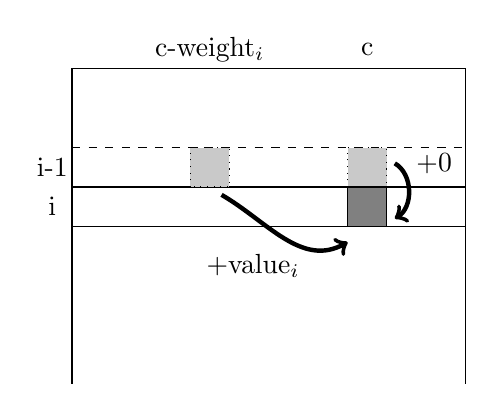
\begin{tikzpicture}
  \draw (15,11) -- (15,15) -- (10,15) -- (10,11);
  \draw[dashed] (10,14) -- (15,14);
  \node at (9.75,13.75) {i-1};
  \node at (9.75,13.25) {i};
  \draw (10,13.5) -- (15,13.5);
  \draw (10,13) -- (15,13);
  \draw[dotted,fill=black!30!white!70] (13.5,13.5) rectangle (14.0,14);
  \draw[dotted,fill=black!30!white!70] (11.5,13.5) rectangle (12.0,14);
  \draw[fill=gray] (13.5,13) rectangle (14.0,13.5);
  \node at (13.75,15.25) {c};
  \node at (11.75,15.25) {c-weight${}_i$};
  \draw[ultra thick,->] (11.9,13.4) to [out=-30,in=210] (13.5,12.8);
  \draw[ultra thick,->] (14.1,13.8) to [out=-30,in=30] (14.1,13.1);
  \node at (14.6, 13.8) {+0};
  \node at (12.3, 12.5) {+value${}_i$};
\end{tikzpicture}
\end{center}

\begin{pbox}{Combinatorial - Knapsack Problem}{AOJ}
In the knapsack problem where each item can be selected any number of times, find the maximum total value that satisfies the constraints.

\aojid{DPL_1_C}
\end{pbox}

The approach is almost the same, but the recurrence relation changes slightly. This knapsack problem without quantity restrictions can be solved with the same computational complexity order $O(NW)$ as the 1-item-limited knapsack problem. If you plan to increase the \texttt{for} loop related to weight by one, making it a triple loop, it will become $O(NW^2)$. Consider how to improve it.

As a similar problem, there is the knapsack problem with quantity restrictions, where each item has a given quantity constraint (bound). By applying the concept of sliding minimum values, a solution can be obtained more efficiently (than solving it as a 0-1 knapsack with increased items) (see also \pccbook[p.~302]).

\paragraph{Longest Common Subsequence and Edit Distance}
A subsequence is a sequence obtained by extracting some elements from a data sequence such as a string (or a sequence obtained by deleting some elements and packing the remaining elements). A common subsequence is a sequence that is a subsequence of both of two data sequences. The longest sequence among the common subsequences is called the \jindex{longest common subsequence}{longest common subsequence}. There may be multiple longest common subsequences.

\begin{pbox}{Dynamic Programming - Longest Common Subsequence}{AOJ}
Find the length of the longest common subsequence.

\aojid{ALDS1_10_C}
\end{pbox}

Approach: Let $X_i$ represent the subsequence obtained by extracting the first $i$ characters of string X. $X_0$ is an empty string. The longest common subsequence of string X and string Y can be found using $L_{i,j}$, the length of the longest common subsequence of $X_i$ and $Y_j$, which is a subproblem.
\begin{equation*}
    L_{i,j} = \left\{
  \begin{array}{ll}
    0 & i \le 0 \text{ or } j \le 0\\
    1 + L_{i-1,j-1} & \text{The }i\text{-th character of X and the }j\text{-th character of Y are the same}\\
    \max(L_{i,j-1},L_{i-1,j}) & \text{otherwise}
  \end{array}\right.
\end{equation*}
This calculation can be performed efficiently using a two-dimensional array. See the "Pattern Recognition" chapter of information science or \pcaojbook[pp.~253--].

Note: It is difficult to fit this problem within the time limit in Python. If you get TLE, it is good to download the data and verify the answer manually.

\begin{pbox}{Combinatorial - Edit Distance (Levenshtein Distance)}{AOJ}
  Find the edit distance between two strings.
  
\aojid{DPL_1_E}
\end{pbox}


\paragraph{Longest Increasing Subsequence}
The longest increasing subsequence is a well-known problem in dynamic programming, and it can be solved in $O(N\log N)$ by combining \texttt{vector} and binary search (see Section \ref{section:binary-search}). See the explanation at the end of the problem or \pcaojbook[pp.~421--].

\begin{pbox}{Combinatorial - Longest Increasing Subsequence}{AOJ}
  Find the Longest Increasing Subsequence.

\aojid{DPL_1_D}
\end{pbox}
\section{Exercises}

\begin{pbox}{Minimal Backgammon}{Asian Regional 2007}
Find the probability of reaching the goal in a Sugoroku game on a straight line.
  
\aojid{1277}
\end{pbox}

\begin{pbox}{Coin Changing Problem}{AOJ}
Find the minimum number of coins needed to pay exactly.

\aojid{DPL_1_A}
\end{pbox}
Note: Japanese coins have the property that the value of a larger coin is divisible by the value of a smaller coin, so it is better to use larger coins as much as possible. That is, if the payment amount exceeds 500 yen, it is better to use a 500 yen coin. On the other hand, this problem also deals with situations where this is not the case. When paying 200 yen with a coin system of 150 yen, 100 yen, and 1 yen coins, using a 150 yen coin does not minimize the number of coins.
See \pcaojbook[pp.~412--].

\begin{pbox}{Eleven Lover$\star$}{Mock Regional 2009}
Count the multiples of 11 in a sequence of digits.
  
\aojid{2182}
\end{pbox}

Example approach: Look at the digits one by one from the left. Focusing on the $i$-th digit, let $A_{i,j}$ be the number of numbers ending at the $i$-th digit that have a remainder of $0 \le j < 11$ when divided by 11. Calculate $A_{i,.}$ from $A_{i-1,.}$ and the value of the $i$-th digit.

\begin{pbox}{Restore Calculation$\star$}{Asian Regional 2013}
Given two integers and their sum, which may contain ?, find the number of ways to fill in the ?'s such that the operation is consistent.

\aojid{2566}
\end{pbox}

\begin{pbox}{Magic Slayer$\star$}{Summer Camp 2009}
Defeat all enemies by skillfully using single-target and area-of-effect magic. Each magic has a specified MP cost and damage, in addition to being single-target or area-of-effect. The enemies are given by their HP values, which indicate how much damage is needed to defeat them.

\aojid{2156}
\end{pbox}

Explanation: \url{http://acm-icpc.aitea.net/index.php?plugin=attach&refer=2009%2FPractice%2F%B2%C6%B9%E7%BD%C9%2F%B9%D6%C9%BE&openfile=2b.pdf}

You can ignore the names of the magic spells.

Consider the case of a single enemy with only single-target magic. Let $A_d$ be the minimum MP required to deal a total damage of $d$. Then,

\begin{equation}
  A_d = \left\{
  \begin{array}{ll}
    0 & d\le 0\\
    \min_k(A_{d-\mbox{Damage}_k} + \mbox{MP}_k) & d > 0 \mbox{ using magic $k$ last}
  \end{array}\right.
\end{equation}

When defeating $N$ enemies with only single-target magic, it is sufficient to sum the required MP for each enemy's HP.

When area-of-effect magic is available, calculate the minimum MP required to deal a total damage of $d$ to all enemies in the same way, and combine them.

\begin{pbox}{Mushrooms$\star$}{Algorithmic Engagements 2010}
Collect mushrooms by walking on a straight line.

\url{https://szkopul.edu.pl/problemset/problem/KVIxa_im2wGYJX99NB31p_nC/site/}
\end{pbox}

Recommended to use scanf.

\begin{pbox}{Rotating Blackout Plan$\star$}{National Preliminary 2011}
Divide the intervals skillfully.

\aojid{1176} 
\end{pbox}

A type that manages values for rectangles.

\begin{pbox}{Quest of Merchant$\star$}{Summer Camp 2011}
Maximize profit by combining various actions (see problem statement).

\aojid{2296}
\end{pbox}

\begin{pbox}{My friends are small}{Summer Camp 2010}
There are $N$ items. How many ways are there to choose a maximal subset of items whose total weight is less than or equal to $W$? $N \le 200, W \le 10\,000$
\aojid{2333}
\end{pbox}

Maximal means that adding any unselected item would exceed $W$.

Approach: Among the unselected items, consider the lightest one and branch based on it. If we calculate the number of ways to choose items with a total weight of $w$ using a knapsack problem in descending order of weight, we can obtain the solution from the information in the solving process.

Explanation: \url{https://drive.google.com/file/d/1WC7Y2Ni-8elttUgorfbix9tO1fvYN3g3/view}

\begin{pbox}{Hakone$\star\star$}{Summer Camp 2012}
From the changes in rankings (e.g., this team moved up in the rankings and passed in 5th place), find the number of possible rankings at the previous relay point (for Hakone Ekiden).

\aojid{2439}
\end{pbox}

\begin{pbox}{Barricades}{Algorithmic Engagements 2007}
Problem: Block off some roads with barricades to make a connected set of k cities inaccessible from other cities.

\url{https://szkopul.edu.pl/problemset/problem/1sX3vqLjiqkpxBNI-sh8UC2m/site/}
\end{pbox}

\begin{pbox}{Army Training$\star\star$}{Algorithmic Engagements 2010}
Given up to 1000 points on a plane, connect them appropriately to form a simple polygon, and count the number of points contained within the area.

\url{https://szkopul.edu.pl/problemset/problem/nXF1qOIv5S88utFPI2V_0gt3/site/}
\end{pbox}
\chapter{Divide and Conquer}\label{chapter:divide-and-conquer}

\begin{itembox}[l]{Overview}
Divide and conquer is a technique that recursively decomposes a problem into smaller subproblems, solves each of them, and then sequentially combines them to obtain the overall solution.
It is similar to dynamic programming in that it deals with problems smaller than the original problem, but divide and conquer handles cases where the divided subproblems do not overlap. For example, binary search is a divide and conquer technique, but the calculation of Fibonacci numbers is not usually called divide and conquer.

This chapter deals with recursion. If you are not familiar with recursion, please refer to Appendix \ref{section:recursion} as needed.
\end{itembox}

In this chapter, be especially careful because i (\texttt{i}) and j (\texttt{j}), and 1 (\texttt{1}) and l (\texttt{l}) are particularly confusing.
\section{Binary Search}\label{section:binary-search}

Let's look at \jindex{binary search}{binary search} as an example of a case where it is sufficient to divide a problem in half and deal with only one side.
For example, consider the case of determining whether an element exists in a data sequence that is ordered, such as a dictionary or a roster.
For instance, when searching for the surname ``Moore'' in a roster with a total of 1024 pages,
start from the middle page, page 512. If that page is after ``M'', search the front. If it is before ``M'', search the back. In either case, the search range can be narrowed down to half.

This search method is faster than searching the roster page by page from the first page to the last.
If the number of pages in the roster is $n$, there is a difference between the number of pages to check, $O(n)$ and $O(\log(n))$.

Note that in merge sort and \texttt{inversion count}, which will be introduced in the next section, it is necessary to process both regions after division.

\subsection{Searching for Values in a Data Sequence}

The \texttt{binary\_search} function, included in the C++ standard library, uses binary search to determine whether an element exists in a sorted array.

\begin{cbox}[emph={sort,binary\_search}]
\begin{verbatim}
#include <iostream>
#include <algorithm>

sort(S, S+L); // Preparation: Sort the array S in ascending order beforehand
...
    if (binary_search(S, S+L, a)) {
       // a is in S
    }
\end{verbatim}
\end{cbox}

If we write the case of searching for \texttt{value} from the array \texttt{A[]} somewhat formally, it would be as follows:
\begin{enumerate}
\setlength{\itemsep}{0pt}
\item Let the interval to search be $[l, r)$ (to represent a range, left, right, or first, last are often used). When searching from page 0 to page 1023, the initial state is \texttt{l=0, r=1024}.
\item If \texttt{l+n <= r}, the search range has at most \texttt{n} pages left, so search the range \texttt{[l,r)} sequentially. (Typically \texttt{n==1}, but in practice, it may be set to around \texttt{n==10}).
\item Find the middle of the interval: \texttt{m=(l+r)/2}.
\item If \texttt{value < A[m]}, (we want to search the first half \texttt{[l,m)} next), set \texttt{r=m}. Otherwise (including the case where \texttt{A[m] <= value}, i.e., \texttt{A[m]==value}), we want to search the second half \texttt{[m,r)}, so set \texttt{l=m} and go to step 2. (Here, if \texttt{m==l} or \texttt{m==r}, it will be an infinite loop. Confirm that this does not happen.)
\end{enumerate}
This is the kind of process that is performed.

\begin{cbox}[emph={left,right}]
\begin{verbatim}
bool bsearch(const int array[], int left, int right, int value) {
    // Assumptions:
    // - array is sorted in ascending order,
    // - the half-open interval [left,right) is a valid range
    // Possibilities
    // A. array[left] <= value <= array[right-1] (answer is possible)
    // B. value <= array[left] (false is certain)
    // C. array[right-1] <= value (false is certain)
    while (left + 1 < right) {
        // Loop invariant: One of A, B, or C that holds at the start of the loop also holds at the end
        int med = (left+right)/2;
        if (array[med] > value) right = med;
        else left = med;
    }
    return left < right && array[left] == value;
}
\end{verbatim}
\end{cbox}

After implementing binary search yourself, you can check its operation with Search II.

There is a concept called \cemph{loop invariant} as a tool for thinking about the correctness of programs that include complex loops. If necessary, please refer to Appendix \ref{chapter:loop-invariants}.

\begin{psbox}{Search II}{AOJ}
Given an array of integers S (a list of items to sell) and T (a list of items to buy).
Output the number of integers in T that are also included in S.

(Input range) The number of elements in S is at most 100,000, and the number of elements in T is at most 50,000.
The number of elements in S and T are each at most 100. The elements included in the arrays are between 0 and $10^7$.

(Note) The elements of T are mutually distinct, but the elements of S may have duplicates.

\aojid{10031}
\end{psbox}

\begin{debugbox}{Pay Attention to the Problem Specifications}
The meaning of "The elements of T are mutually distinct, but the elements of S may have duplicates" is that if \texttt{S=[1,1,1], T={1}}, then the answer is 1.
\end{debugbox}
\subsection{Finding the Minimum Value that Satisfies a Constraint}

Besides situations where we search for a value in an array, there are problems that can be solved elegantly using the concept of binary search.

\begin{psbox}{Search - Allocation}{AOJ}
Consider loading items of various weights onto trucks in the order they are arranged. Assume the weights of the items are stored in an array \texttt{w} in the order they are arranged.
Assume that all trucks have the same maximum load capacity. What is the minimum maximum load capacity required for each truck to load all the items onto \texttt{k} trucks in order?
Find the minimum value of the "maximum load capacity of the truck".

\aojid{ALDS1_4_D}
\end{psbox}

Hint: Perform a binary search on the maximum load capacity P of the truck to find the minimum value that allows all items to be loaded.
Since the value we are looking for, "the minimum value that allows loading", is an integer, we can find "the maximum value that does not allow loading" and add 1, because "the minimum value that allows loading" = "the maximum value that does not allow loading" + 1.
Represent the range where "the maximum value that does not allow loading" exists as \texttt{[l,h)}, and express the condition for reducing the upper bound \texttt{h} as \texttt{ok}. The answer we are looking for is \texttt{h}.
\begin{cbox}[emph={l,h}]
\begin{verbatim}
bool ok(int P) {
  ... // Returns whether the number of trucks needed when loading in order with a maximum load capacity of P is within K.
}
int main() {
    // Read the problem
    int l = 0, h = // A large number;
    while (l+1 < h) {
        // Loop invariant: Cannot load with l, can load with h
        int m = (l+h)/2;
        if (ok(m)) h = m; else l = m;
    }
    printf("%d\n", h);
}
\end{verbatim}
\end{cbox}

The function \texttt{ok} can be created as follows, for example:
\begin{itemize}
    \item Create variables representing the weight loaded on the current truck (initial value 0) and the number of trucks (initial value 1).
    \item For each item, if loading it onto the current truck does not exceed the maximum load capacity, load it (increase the weight loaded on the current truck). Otherwise, load it onto a new truck (increase the number of trucks and set the weight loaded on the current truck to that item).
    \item Finally, compare the number of trucks with K.
\end{itemize}

\begin{psbox}{Aggressive Cows$\star$}{USACO 2005 February Gold}
There are N stalls (individual rooms) for cows on a straight line. We want to place C cows as far apart from each other as possible.

(Please use scanf instead of cin)

\url{http://poj.org/problem?id=2456}
\end{psbox}

This time, since we want the maximum value that satisfies the condition, we express the condition for increasing the lower bound \texttt{l} as a function \texttt{ok}. The answer we are looking for is \texttt{l}.
If we sort the candidate stalls in ascending order beforehand, the \texttt{ok} function can be implemented as follows:
\begin{itemize}
    \item Place a cow in the leftmost stall (fail if there are no stalls).
    \item Remove stalls within a distance of M from consideration.
\end{itemize}
Repeat these steps for the number of cows, and if all cows can be placed, it can be judged as a success.

\begin{psbox}{Water Tank}{Mock Regional Preliminary 2009}
Given the capacity of a tank and the amount of water used per hour, find the minimum required water supply rate. (The amount that does not lead to a gradual decline even after multiple cycles is required).

(Note that there is another problem with the same name)

\aojid{2180}
\end{psbox}

Assume a certain water supply rate, and let \texttt{ok} be a function that determines whether it is possible to live with that rate. Represent the interval containing the required rate as $[\text{lo},\text{hi}]$, and narrow the range in half depending on whether it is possible to live or not. When the interval becomes sufficiently narrow, terminate and output the result. The concept and effect are almost the same as binary search, but when dealing with continuous intervals, it is often called bisection.

\begin{cbox}
\begin{verbatim}
  double lo = sum/86400, hi = 1e6; // 1e6 = $10^6$
  while (hi-lo>1e-6) {
      double m = (hi+lo)/2.0;
      if (ok(m)) hi = m;
      else lo = m;
  }
  printf("%.10f\n", hi);
\end{verbatim}
\end{cbox}

The principle is simple, but in the implementation of the function \texttt{ok}, it is necessary to be careful in handling cases such as not being able to store water beyond the maximum capacity of the tank. Therefore, the problem of inversion count in the next section might be easier.
\section{Merge Sort}
As an example of divide and conquer, we will discuss a sorting method called Merge Sort. This method divides a given array in half and sorts the elements when assembling it back to its original size. The figure shows the flow of processing when sorting the array 8, 1, 4, 3, 2, 5, 7, 6. The division occurs in the upper half, and the sorting occurs in the lower half. The red numbers indicate elements that came from the right side during merging.
The specific source code is almost the same as the \texttt{merge\_and\_count} introduced next, so it is omitted. If the number of elements in the array is $N$, there are $O(\log N)$ rows, and the calculation required for each row is $O(N)$, so the overall computational complexity is $O(N\log N)$.

\begin{center}
      \begin{tikzpicture}[node distance=18.4mm,
          merge/.style={
            draw=igreen,
            minimum size=7mm,
            ultra thick,
            inner sep=4pt
        }]
        \node[city] (A)              {8,1,4,3,2,5,7,6};
        \node[city] (B) [below left of=A] {8,1,4,3};
        \node[city] (C) [below right of=A] {2,5,7,6};
        \node[city] (E) [below left of=B] {4,3};
        \node[city] (D) [left of=E] {8,1};
        \node[city] (F) [below right of=C] {2,5};
        \node[city] (G) [right of=F] {7,6};
        \node[city] (I) [below left of=D] {1};
        \node[city] (H) [left of=I] {8};
        \node[city] (K) [below right of=E] {3};
        \node[city] (J) [left of=K] {4};
        \node[city] (L) [below left of=F] {2};
        \node[city] (M) [right of=L] {5};
        \node[city] (N) [below right of=G] {7};
        \node[city] (O) [right of=N] {6};
        \node[merge] (P) [below right of=I] {\textcolor{ired}{1},8};
        \node[merge] (Q) [right of=P] {\textcolor{ired}{3},4};
        \node[merge] (R) [below right of=L] {2,\textcolor{ired}{5}};
        \node[merge] (S) [right of=R] {\textcolor{ired}{6},7};
        \node[merge] (T) [below right of=Q] {1,\textcolor{ired}{3,4},8};
        \node[merge] (U) [below left of=R] {2,5,\textcolor{ired}{6,7}};
        \node[merge] (V) [below right of=T] {1,\textcolor{ired}{2},3,4,\textcolor{ired}{5,6,7},8};
        \path[->,thick] (A) edge (B);
        \path[->,thick] (A) edge (C);
        \path[->,thick] (B) edge (D);
        \path[->,thick] (B) edge (E);
        \path[->,thick] (C) edge (F);
        \path[->,thick] (C) edge (G);
        \path[->,thick] (D) edge (H);
        \path[->,thick] (D) edge (I);
        \path[->,thick] (E) edge (J);
        \path[->,thick] (E) edge (K);
        \path[->,thick] (F) edge (L);
        \path[->,thick] (F) edge (M);
        \path[->,thick] (G) edge (N);
        \path[->,thick] (G) edge (O);
        \path[->,thick] (H) edge (P);
        \path[->,thick] (I) edge (P);
        \path[->,thick] (J) edge (Q);
        \path[->,thick] (K) edge (Q);
        \path[->,thick] (L) edge (R);
        \path[->,thick] (M) edge (R);
        \path[->,thick] (N) edge (S);
        \path[->,thick] (O) edge (S);
        \path[->,thick] (P) edge (T);
        \path[->,thick] (Q) edge (T);
        \path[->,thick] (R) edge (U);
        \path[->,thick] (S) edge (U);
        \path[->,thick] (T) edge (V);
        \path[->,thick] (U) edge (V);
      \end{tikzpicture}
\end{center}
\subsection{Inversion Count}

We want to count the number of pairs of elements in an array such that \texttt{A[i] > A[j] (i<j)}.
For example, in the array \texttt{[3 1 2]}, there are two pairs with reversed order: (3,1) and (3,2).
If we naively write the following code, it will take time proportional to the square of the number of elements $N$, i.e., $O(N^2)$.

\begin{cbox}
int N, A[128];
int solve() {
    int sum = 0;
    for (int i=0; i<N; i++)
        for (int j=i+1; j<N; j++)
            if (A[i] > A[j]) ++sum;
    return sum;
}
\end{cbox}

By applying merge sort and counting while dividing in half, it can be found in $O(N\log N)$.

\begin{cbox}[emph={merge\_and\_count}]
int N, A[lots]; // A is the original array
int W[lots]; // W is a work array
int merge\_and\_count(int l, int r) { // range [l,r)
    if (l+1 >= r) return 0; // empty
    if (l+2 == r) { // [l,r) == [l,l+1] only 2 elements
        if (A[l] <= A[l+1]) return 0;  // no inversion
        std::swap(A[l], A[l+1]);
        return 1; // one inversion
    }
    int m = (l+r)/2; // [l,r) == [l,m) + [m,r)
    int cl = merge\_and\_count(l, m); // recursively count the left half
    int cr = merge\_and\_count(m, r); // recursively count the right half
    int c = 0; // number of inversions when merging left and right
    int i=l, j=m; // i moves in [l,m), j moves in [m,r),
    int k=l;      // write smaller elements to W[k]
    while (i<m && j<r) { // compare A[i] and A[j] while moving
        if (A[i] <= A[j]) W[k++] = A[i++]; // left half is smaller, no inversion
        else {
            W[k++] = A[j++];
            c += m - i; // left half is larger, skip unprocessed elements in the left half
        }
    }
    while (i<m) W[k++] = A[i++]; // if left half remains
    while (j<r) W[k++] = A[j++]; // if right half remains
    assert(k == r);
    std::copy(W+l, W+r, A+l);
    return cl + cr + c;
}
\end{cbox}
\subsection{Exercises}

\begin{pbox}{Recursion / Divide and Conquer - The Number of Inversions}{AOJ}
Find the number of pairs in a given sequence where the order of magnitude is reversed.

\aojid{ALDS1_5_D}
\end{pbox}

\begin{pbox}{Ultra-QuickSort}{Waterloo local 2005.02.05}
Similar problem: Use \texttt{long long} because the numbers are large.

\url{http://poj.org/problem?id=2299} 
\end{pbox}

\begin{pbox}{Japan$\star$}{Southeastern Europe 2006}
Roads run east-west on a rectangular island. Find the number of intersections.

\url{http://poj.org/problem?id=3067}
\end{pbox}

Example solution: If you sort by (East, West) pairs, it becomes the same problem as the previous two. This problem can also be solved by managing cumulative sums.
\section{Tree Traversal}

\begin{center}
\begin{tabular}{c}
  \begin{forest}
    ctree [$D_{1,7,13}$ [$B_{2,4,6}$ [$A_3$] [$C_5$]] [$E_{8,12}$
        [nil,cnil] [$G_{9,11}$ [$F_{10}$], [nil,cnil]]]]
  \end{forest}
\\
Example 1: Numbers represent the order of visitation
\end{tabular}
\end{center}

Starting from the root, consider traversing each vertex once while following the edges using the following recursive procedure (depth-first search, Chapter \ref{section:graphsearch}):
\begin{enumerate}
\setlength{\itemsep}{0pt}
\item If a left child exists and has not been visited, visit the left child.
\item (Otherwise) If a right child exists and has not been visited, visit the right child.
\item (Otherwise) If there is a parent, return to the parent.
\item If none of the above, (since we have returned to the root) terminate.
\end{enumerate}

For the tree in "Example 1" in the figure, the path would be DBABCBDEGFGED.
As can be seen from the example, vertices with children are visited multiple times (specifically, the degree of the vertex).

Based on this visitation order, methods for processing each vertex only once include preorder (self, left, right), inorder (left, self, right), and postorder (left, right, self). Each method has a different priority order between children and self.

\begin{center}  
\begin{tabular}{ll}\hline
 & DBABCBDEGFGED\\\hline
preorder & DBA\phantom{B}C\phantom{B}\phantom{D}EGF\phantom{GED}\\
inorder  & \phantom{DB}ABC\phantom{B}DE\phantom{G}FG\phantom{ED}\\
postorder &\phantom{DB}A\phantom{B}CB\phantom{DEG}FGED\\
\hline
\end{tabular}
\end{center}

\begin{pbox}{Tree - Reconstruction of a Tree}{AOJ}
For a certain binary tree, the list of vertices output in preorder (root, left, right) and the list output in inorder (left, root, right) are given.
(Restore the original tree) and output its vertices in postorder (left, right, root).
Note that in the original tree, different vertices have different labels.

  \aojid{ALDS1_7_D}
\end{pbox}

\begin{pbox}{Tree Recovery$\star$}{Ulm Local 1997}
Same as above (except that multiple cases are given and the format is slightly different).

\url{http://poj.org/problem?id=2255}  
\end{pbox}


Hint:
\begin{itemize}
\setlength{\itemsep}{0pt}
\item Let the root be A, the left subtree be L (which may be null), and the right subtree be R. In preorder, they are arranged as AL'R'. (L' and R' are their respective preorder notations). In inorder, they are arranged as L''AR'' (L'' and R'' are their respective inorder notations).
\item The root A can be immediately identified from the beginning of the preorder notation.
\item The L and R parts can be identified by searching for A in the inorder notation.
\item Note that the number of characters is the same for L' and L'', and for R' and R''.
\item The problem of restoring the left tree from L' and L'' is a smaller version of the original problem.
\end{itemize}

Example solution:

\begin{cbox}
\begin{verbatim}
#include <iostream>
#include <string>
using namespace std;
string preorder, inorder;
// For the range [fp,lp) of preorder and the range [fi,li) of inorder,
// display the tree in postorder
void recover(int fp, int lp, int fi, int li) {
    int root;
    // Find the root such that preorder[fp] == inorder[root]
    if (/* If the left side exists */ fp+1 < lp && fi < li)
      recover(fp+1, fp+(root-fi)+1, fi, root); // Display the left side
    if (/* If the right side exists */ fp+(root-fi)+1 < lp && root+1 < li)
      recover(fp+(root-fi)+1, lp, root+1, li); // Display the right side
    cout << inorder[root]; // Display the root
}
int main() {
    while (cin >> preorder >> inorder) {
        recover(0, preorder.size(), 0, inorder.size());
        cout << endl;
    }
}
\end{verbatim}
\end{cbox}

The call relationship can be visualized as follows. In the figure, the red characters represent the root (in the subtree at that point). The strings inside the vertices are the preorder notation (top, range of fp and lp) and the inorder notation (bottom, range of fi and li) for the subtree below that vertex.

\begin{center}
\begin{forest}
  sn edges
  [\vbox{\hbox{\textcolor{ired}{D}BACEGF}\hbox{ABC\textcolor{ired}{D}EFG}}
  [\vbox{\hbox{\textcolor{ired}{B}AC}\hbox{A\textcolor{ired}{B}C}}
    [A][C]]
  [\vbox{\hbox{\textcolor{ired}{E}GF}\hbox{\textcolor{ired}{E}FG}}
  [nil,cnil]
  [\vbox{\hbox{\textcolor{ired}{G}F}\hbox{F\textcolor{ired}{G}}} [F] [nil,cnil]]]]
\end{forest}
\end{center}
\section{Space-Filling Curves}
\begin{pbox}{Recursion / Divide and Conquer - Koch Curve}{AOJ}
  \begin{minipage}{.7\linewidth}
Compute the vertices of the Koch curve.
  
\aojid{ALDS1_5_C}
  \end{minipage}
\begin{tikzpicture}[decoration=Koch snowflake]
    \draw decorate{ decorate{ decorate{ decorate{ (0,0) -- (3,0) }}}};
\end{tikzpicture}
\end{pbox}

Hint: When a base line is drawn from $(x0,y0)$ to $(x0+dx,y0+dy)$, to create a bulge on the left side, extend an appropriate distance from the midpoint $(x0+dx/2,y0+dy/2)$ in the $(-dy,dx)$ direction.

There are two approaches to designing a recursive function to draw the \jindex{Koch curve}{Koch curve}: one is a design that displays the curve, and the other is a design that returns a sequence of points.

If we design a function \tindex{koch}\texttt{(x0,y0,x1,y1,n)} to "display the points from coordinates (x0,y0) to (x1,y1) (the endpoints include (x0,y0) but not (x1,y1))", the structure would be as follows:
\begin{pybox}
import math
def show_vertex(x,y):
    print("
def koch(x0,y0, x1,y1, n):
    if n == 0:
        show_vertex(x0,y0)
    else:
        ... # Calculate intermediate points c1, c2, c3
        koch(x0,y0, c1[0],c1[1], n-1)
        koch(c1[0],c1[1], c2[0],c2[1], n-1)
        koch(c2[0],c2[1], c3[0],c3[1], n-1)
        koch(c3[0],c3[1], x1,y1, n-1)

N = int(input())
koch(0,0,100,0,N)
show_vertex(100,0)
\end{pybox}

In the case of returning a sequence of points, it can be written as follows (display all at once after the entire calculation is finished):
\begin{pybox}
def koch(x0,y0, x1,y1, n):
    if n == 0:
        return [(x0,y0)]
    else:
        ... # Calculate intermediate points c1, c2, c3
        return koch(x0,y0, c1[0],c1[1], n-1) \
            + koch(c1[0],c1[1], c2[0],c2[1], n-1) \
            + koch(c2[0],c2[1], c3[0],c3[1], n-1) \
            + koch(c3[0],c3[1], x1,y1, n-1)

def show_vertex(x,y):
    print("

N = int(input())
V = koch(0,0,100,0,N)+[[100,0]]
for x,y in V:
    show_vertex(x,y)
\end{pybox}

In C++, since the implementation of the latter design is cumbersome, the former design (displaying within the recursive function) is simpler.

\begin{tipsbox}{Visualizing Point Sequences}
  When the answer is incorrect or you are struggling with the approach, it is good to visualize the point sequence.
In an environment where \tindex{gnuplot} is available, it can be easily visualized using the following procedure.
(1) Start gnuplot in the terminal. (2) At the gnuplot prompt, type \texttt{plot 'xy.txt' with lines}. Assume that the coordinates output by the program are saved in ``xy.txt''.
\begin{terminal}
\$ gnuplot
gnuplot> plot 'xy.txt' with lines
\end{terminal}
\end{tipsbox}
Also, in the case of Python, \tindex{matplotlib} is convenient to use.
\begin{pybox}
import matplotlib.pyplot as plt
import numpy as np
def plot_koch(a):
    fig = plt.figure()
    ax = fig.add_subplot(1,1,1)
    a_ = np.array(a)
    xlist = a_[:, 0]
    ylist = a_[:, 1]
    ax.plot(xlist, ylist)
    ax.set_title('koch curve')
\end{pybox}
(To display within jupyter, execute \texttt{\%matplotlib inline} at the beginning)

\begin{pbox}{Riding the Bus$\star\star$}{World Finals 2003}

There are grid points on a Peano curve drawn within a square. Find the distance between two given points. The distance is the distance from the given point to the nearest grid point (or the one with the smallest x,y coordinates if there are multiple), and the distance along the Peano curve between the grid points. (The description of the error is a bit concerning)

\url{https://icpcarchive.ecs.baylor.edu/index.php?option=com_onlinejudge&Itemid=8&category=37&page=show_problem&problem=724}
\end{pbox}

Example solution: Divide the whole into 9 parts, and search in detail only in the relevant areas.

\begin{pbox}{Plotter$\star\star$}{Algorithmic Engagements 2011}
When does the pen pass through a given point?
  
\url{http://main.edu.pl/en/archive/pa/2011/plo}
\end{pbox}
\chapter{Basic Data Structures (string, stack, queue, string, set, map)}\label{chapter:datastructure}

\begin{itembox}[l]{Overview}
In this chapter, we introduce strings, stacks, (priority) queues, sets, and associative arrays as "tools" provided as standard libraries in many languages such as C++ and Java.
Readers who find the introduction of tools boring can skip ahead and come back later when needed. In this material, we take the position of first recommending the use of standard libraries. Creating these tools yourself is useful as strength training, but it is not suitable for beginners. Also, in practical situations, it is preferable to use standard libraries if they are sufficient.
For example, there are benefits such as expecting no bugs because they are used by many people, and they are suitable for collaborative work because other people know their properties well.

In this chapter, we will cover sample code for C++ and Python3. For Ruby, please refer to Appendix \ref{chapter:ruby}.
\end{itembox}
\section{Strings and Input/Output}

\begin{cbox}[emph={string}]
\begin{verbatim}
#include <iostream>
#include <string>
using namespace std;
int main() {
  string word; // Defines a string variable named word
  cin >> word; // Reads one word from standard input (delimited by spaces or newlines)
  cout << word << word << endl; // Displays it twice
}
\end{verbatim}
\end{cbox}

If you input \texttt{hello}(newline), it will output \texttt{hellohello}.

The C++ string class is much more convenient than C-style strings, so it is recommended to get used to it early.

\begin{cbox}
\begin{verbatim}
#include <string>
  string word; // Definition
  string word2="ABCD"; // Definition and initialization
  word = "EF"; // Assignment
  string word3 = word + word2; // Concatenation
  char c = word[n]; // Extracts the n-th character
  word[n] = 'K'; // Assigns to the n-th character (fails if \texttt{n<word.size()} is not satisfied)
  cin >> word; // Reads one word (separated by newlines or spaces)
  cout << word.size() << endl; // Displays the number of characters
  if (word.find("A") != string::npos) ... // If word contains A...
\end{verbatim}
\end{cbox}

\begin{pybox}
\begin{verbatim}
word = input().strip()
print(word*2)
\end{verbatim}
\end{pybox}

Reading one word and reading one line have different meanings, but we will not delve into the difference this time.
\section{Stacks and Queues}

Stacks and queues (\pcaojbook[pp.~80--], \pccbook[pp.~31--]) are data structures for temporarily storing and retrieving data. Both manage data in a single line, storing new data at one end of the line (either end), and also retrieving data from one end (either end).

A \jindex{stack}{stack} is a data structure where the data stored later is retrieved first. For example, it is useful in situations where an urgent task arises while working, so the current task is placed at the top of a "pile of work," the urgent task is processed, and when that is finished, the process is resumed from the top of the pile of work. Of course, if another urgent task arises while processing an urgent task, it is similarly added to or removed from the pile of work.

A \jindex{queue}{queue} is a data structure where the data stored earlier is retrieved first. This corresponds to the situation where people arriving at a restaurant line up at the back of the queue, and people are guided into the restaurant in the order they arrived earliest in the queue.

In a \jindex{priority queue}{priority queue}, data is retrieved in order of priority, not in the order they were queued. Although there is no perfect real-world example, it would correspond to a situation where patients are treated in order of priority from among those waiting, or a market where items can be obtained in order of the highest bid.

Note that in the C++ standard library, the retrieval operation is separated into two operations: referencing the first element \texttt{top()} or \texttt{front()} and removing the first element \texttt{pop()}\footnote{This is for exception safety.}. In normal usage, we want to obtain the first element and remove it from the stack or queue, so we perform both operations consecutively.
\subsection{Stacks}\label{section:stack}

\paragraph{Overview}
A stack (\eindex{stack}) is a data structure that provides two operations: \tindex{push}\texttt{()} and \tindex{pop}\texttt{()}.
These operations add and remove data, respectively.
The data currently at the top can be referenced using \tindex{top}\texttt{()}.

\centerline{\begin{tabular}{c@{\hspace{2em}}c@{\hspace{2em}}c@{\hspace{2em}}c@{\hspace{2em}}c}
\imagetop{\begin{tikzpicture}
\phantom{\draw (0,1.4) -- (0,0);}
\draw[thick] (0,0) -- (2,0);
\end{tikzpicture}}
&
\imagetop{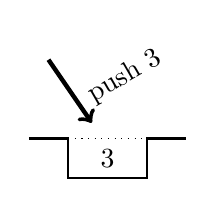
\begin{tikzpicture}
\phantom{\draw (0,1.4) -- (0,0);}
\draw[ultra thick,->] (0.25,1) -- (0.8,0.2) node [above right,rotate=30] {push 3};
\draw[thick] (0,0) -- (0.5,0) -- (0.5,-.5) -- (1.5,-.5) -- (1.5,0) -- (2,0);
\draw[dotted] (0.5,0) -- (1.5,0);
\node at (1,-0.25) {$3$};
\end{tikzpicture}}
&
\imagetop{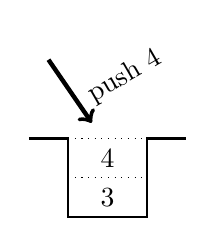
\begin{tikzpicture}
\phantom{\draw (0,1.4) -- (0,0);}
\draw[ultra thick,->] (0.25,1) -- (0.8,0.2) node [above right,rotate=30] {push 4};
\draw[thick] (0,0) -- (0.5,0) -- (0.5,-1) -- (1.5,-1) -- (1.5,0) -- (2,0);
\draw[dotted] (0.5,0) -- (1.5,0);
\draw[dotted] (0.5,-0.5) -- (1.5,-0.5);
\node at (1,-0.25) {$4$};
\node at (1,-0.75) {$3$};
\end{tikzpicture}}
&
\imagetop{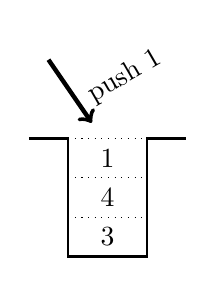
\begin{tikzpicture}
\phantom{\draw (0,1.4) -- (0,0);}
\draw[ultra thick,->] (0.25,1) -- (0.8,0.2) node [above right,rotate=30] {push 1};
\draw[thick] (0,0) -- (0.5,0) -- (0.5,-1.5) -- (1.5,-1.5) -- (1.5,0) -- (2,0);
\draw[dotted] (0.5,0) -- (1.5,0);
\draw[dotted] (0.5,-0.5) -- (1.5,-0.5);
\draw[dotted] (0.5,-1) -- (1.5,-1);
\node at (1,-0.25) {$1$};
\node at (1,-0.75) {$4$};
\node at (1,-1.25) {$3$};
\end{tikzpicture}}
&
\imagetop{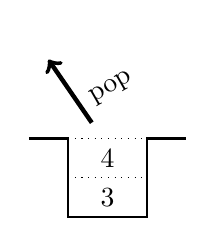
\begin{tikzpicture}
\phantom{\draw (0,1.4) -- (0,0);}
\draw[ultra thick,<-] (0.25,1) -- (0.8,0.2) node [above right,rotate=30] {pop};
\draw[thick] (0,0) -- (0.5,0) -- (0.5,-1) -- (1.5,-1) -- (1.5,0) -- (2,0);
\draw[dotted] (0.5,0) -- (1.5,0);
\draw[dotted] (0.5,-0.5) -- (1.5,-0.5);
\node at (1,-0.25) {$4$};
\node at (1,-0.75) {$3$};
\end{tikzpicture}}
\\
(empty) & top$=3$ & top$=4$ & top$=1$ & top$=4$
\end{tabular}}

\paragraph{Usage Notes}
Usually, arrays or \texttt{vector}s are used.
The computational cost for typical implementations of \texttt{push()}, \texttt{pop()}, and \texttt{top()} is constant time. That is, it is expected that the computation time for each operation will not increase, no matter how much the data increases.

Note that while some implementations of \texttt{pop()} return a value like \texttt{top()}, in the C++ standard library, these are separated\footnote{This is for exception safety.}. In normal usage, we want to get the first element and remove it from the stack or queue, so we perform both operations consecutively.

Also, member functions such as \texttt{size()} to check the current number of elements are provided, so please refer to a grammar book for details\footnote{There is also information on the web: \url{http://en.cppreference.com/w/cpp/container/stack}}.

\begin{cbox}[emph={stack,push,top,pop}]
\begin{verbatim}
#include <stack>
#include <iostream>
using namespace std;
int main() {
    stack<int> S; // Stack to store ints
    S.push(3); // Add to the top
    S.push(4);
    S.push(1);
    while (! S.empty()) { // While there are elements
	int n = S.top(); // Copy the top element
	S.pop(); // Discard the top element
	cout << n << endl; // Displays 1, 4, 3 in that order
    }
}  
\end{verbatim}
\end{cbox}

In Python, we will use \texttt{append} and \texttt{pop} as \texttt{push} and \texttt{pop}, respectively.
\begin{pybox}[emph={append,pop}]
\begin{verbatim}
stack = []
stack.append(3)
stack.append(4)
stack.append(1)
while len(stack) > 0:
    n = stack.pop()
    print(n)
\end{verbatim}
\end{pybox}

\begin{psbox}{Reverse Polish Notation}{AOJ}
Read a grammar given in "Reverse Polish Notation" and calculate the value.
  
\aojid{ALDS1_3_A}
\end{psbox}

Hint: Also refer to the "Explanation" at the end of the problem statement.
A detailed explanation is given in \pcaojbook[p.82].

\begin{cbox}[emph={string,stack,top,push}]
\begin{verbatim}
#include <string>
#include <stack>
#include <iostream>
using namespace std;
int main() {
  string word;
  stack<int> S;
  while (cin >> word) { // Read as long as there is input
    if (word == "+") {
      // pop two numbers, push the sum
    }
    else if (word == "-") {
      // pop two numbers, push the difference
    }
    else if (word == "*") {
      // pop two numbers, push the product
    }
    else {
      // convert word to a number and push it
    }
  }
  // Display the top element of S.
}
\end{verbatim}
\end{cbox}

This program reads as long as the input continues. To give the end of input from the keyboard, use ``\textasciicircum{}D'' (press ``d'' while holding down the Ctrl key).

To convert a string representing a number to an integer \texttt{n},
in C++11, use \texttt{int n=stoi(word)},
otherwise, include \texttt{<cstdlib>} and use \texttt{int n=atoi(word.c\_str())} etc. (AOJ's C++11 does not yet support \texttt{stoi}, so use \texttt{atoi}).

\begin{pbox}{Largest Rectangle in a Histogram}{Ulm Local 2003}
  Find the area of the largest rectangle contained within a histogram. (Note: use long long)

\url{http://poj.org/problem?id=2559}
\end{pbox}

By skillfully utilizing a stack, it can be found in time proportional to the number of bars in the histogram.

Reference: \url{http://algorithms.blog55.fc2.com/blog-entry-132.html}
\subsection{Queues}\label{section:queue}
\paragraph{Overview}
A queue (\eindex{queue},\pccbook[p.~32]) is a data structure that allows data to be stored (\texttt{push()}) and retrieved (\texttt{pop()}).
The data currently at the front can be referenced using \tindex{front}\texttt{()}.

\centerline{\begin{tabular}{c@{\hspace{2em}}c@{\hspace{2em}}c@{\hspace{2em}}c@{\hspace{2em}}c}
\imagetop{\begin{tikzpicture}
\phantom{\draw (0,1.0) -- (0,0);}
\draw[thick] (0,0) -- (2,0);
\end{tikzpicture}}
&
\imagetop{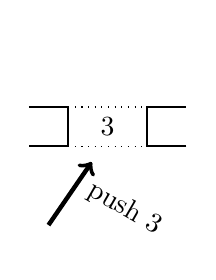
\begin{tikzpicture}
\phantom{\draw (0,1.0) -- (0,0);}
\draw[ultra thick,->] (0.25,-1.5) -- (0.8,-0.7) node [below right,rotate=-30] {push 3};
\draw[thick] (0,0) -- (0.5,0) -- (0.5,-.5) -- (0,-.5);
\draw[thick] (2,-.5) -- (1.5,-.5) -- (1.5,0) -- (2,0);
\draw[dotted] (0.5,0) -- (1.5,0);
\draw[dotted] (0.5,-0.5) -- (1.5,-0.5);
\node at (1,-0.25) {$3$};
\end{tikzpicture}}
&
\imagetop{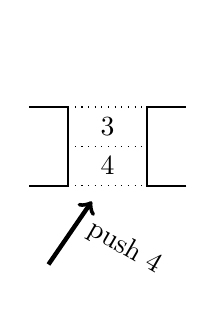
\begin{tikzpicture}
\phantom{\draw (0,1.0) -- (0,0);}
\draw[ultra thick,->] (0.25,-2) -- (0.8,-1.2) node [below right,rotate=-30] {push 4};
\draw[thick] (0,0) -- (0.5,0) -- (0.5,-1) -- (0,-1);
\draw[thick] (2,-1) -- (1.5,-1) -- (1.5,0) -- (2,0);
\draw[dotted] (0.5,0) -- (1.5,0);
\draw[dotted] (0.5,-0.5) -- (1.5,-0.5);
\draw[dotted] (0.5,-1) -- (1.5,-1);
\node at (1,-0.25) {$3$};
\node at (1,-0.75) {$4$};
\end{tikzpicture}}
&
\imagetop{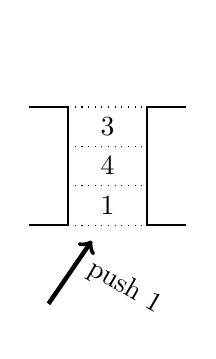
\begin{tikzpicture}
\phantom{\draw (0,1.0) -- (0,0);}
\draw[ultra thick,->] (0.25,-2.5) -- (0.8,-1.7) node [below right,rotate=-30] {push 1};
\draw[thick] (0,0) -- (0.5,0) -- (0.5,-1.5) -- (0,-1.5);
\draw[thick] (2,-1.5) -- (1.5,-1.5) -- (1.5,0) -- (2,0);
\draw[dotted] (0.5,0) -- (1.5,0);
\draw[dotted] (0.5,-0.5) -- (1.5,-0.5);
\draw[dotted] (0.5,-1) -- (1.5,-1);
\draw[dotted] (0.5,-1.5) -- (1.5,-1.5);
\node at (1,-0.25) {$3$};
\node at (1,-0.75) {$4$};
\node at (1,-1.25) {$1$};
\end{tikzpicture}}
&
\imagetop{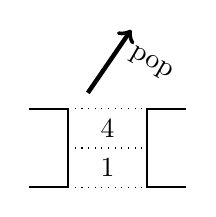
\begin{tikzpicture}
\phantom{\draw (0,1.0) -- (0,0);}
\draw[ultra thick,->] (0.75,0.2) -- (1.3,1) node [below right,rotate=-30] {pop};
\draw[thick] (0,0) -- (0.5,0) -- (0.5,-1) -- (0,-1);
\draw[thick] (2,-1) -- (1.5,-1) -- (1.5,0) -- (2,0);
\draw[dotted] (0.5,0) -- (1.5,0);
\draw[dotted] (0.5,-0.5) -- (1.5,-0.5);
\draw[dotted] (0.5,-1) -- (1.5,-1);
\node at (1,-0.25) {$4$};
\node at (1,-0.75) {$1$};
\end{tikzpicture}}
\\
(empty) & front$=3$ & front$=3$ & front$=3$ & front$=4$
\end{tabular}}

\paragraph{Usage Notes}
Arrays or \tindex{deque}s are used for implementation.
The computational cost for \texttt{push()}, \texttt{pop()}, and \texttt{front()} is constant time. That is, it is expected that the computation time for each operation will not increase, no matter how much the data increases.
(Since moving the entire data would take $O(N)$, in practice, only indices or pointers representing the currently used section, such as head and tail, are manipulated).

In C++, a template class called \texttt{queue} is provided. The data that is put in (pushed) is retrieved by the \texttt{front()} and \texttt{pop()} operations.\footnote{\url{http://en.cppreference.com/w/cpp/container/queue}}
\begin{cbox}[emph={queue,push,front,pop}]
\begin{verbatim}
#include <queue>
#include <iostream>
using namespace std;
int main() {
    queue<int> Q; // Queue to store ints
    Q.push(3); // Add to the end
    Q.push(4);
    Q.push(1);
    while (! Q.empty()) { // While there are elements
	int n = Q.front(); // Copy the first element
	Q.pop(); // Discard the first element
	cout << n << endl; // Displays 3, 4, 1 in that order
    }
}
\end{verbatim}
\end{cbox}

In this material, we will use \texttt{collections.deque}'s \texttt{append, popleft} as the representation of a queue in Python.\footnote{https://docs.python.jp/3/library/collections.html\#deque-objects}
\begin{pybox}[emph={append,popleft}]
\begin{verbatim}
import collections
q = collections.deque()
q.append(3)
q.append(4)
q.append(1)
while len(q) > 0:
    n = q.popleft() # Retrieve from the front
    print(n)
\end{verbatim}
\end{pybox}


\begin{psbox}{Round-Robin Scheduling}{AOJ}
Let's simulate the process of processing multiple calculations little by little.
  
\aojid{ALDS1_3_B}
\end{psbox}

Hint: Also refer to the "Explanation" at the end of the problem statement. A detailed explanation is given in \pcaojbook[p.82].

\begin{pbox}{Areas on the Cross-Section Diagram}{AOJ}
Output the area of the puddles that form when it rains on a given terrain.
  
\aojid{ALDS1_3_D}
\end{pbox}

Hint: If a water surface is formed, it is the most recent pair of a downward slope and an upward slope at the same height.
By looking at the string from left to right,
\begin{itemize}
\item \textcolor{white}{If it is a downward slope, put the position on the stack}
\item \textcolor{white}{If it is an upward slope, pair it with the downward slope that is the top element of the stack, and remove it from the stack}
\end{itemize}
By doing this, it is possible to create pairs of downward and upward slopes at the same height. After that, it is good to remove the water surfaces that are hidden. For example, represent the start position and area with \texttt{pair<int,int>} and manage them with a \texttt{stack}.

\begin{pbox}{Subsequence}{Southeastern Europe 2006}
For a contiguous subsequence of array A, find the minimum length of a subsequence whose sum is greater than or equal to S.

\url{http://poj.org/problem?id=3061}
\end{pbox}

Explanation of the sample: The part (10,7) satisfies the condition $17 \ge 15$ and has the minimum number of elements, which is 2.
The part (3,4,5) satisfies the condition $12 \ge 11$ and has the minimum number of elements, which is 3.

Hint: Checking all intervals takes $O(N^2)$, but by checking only the intervals where the sum is close to $S$ as follows, it can be processed in $O(N)$. Look at the elements of the array in order from the first element, and if the sum of the elements inside the queue is less than S, \texttt{push} to increase the number of elements, and if it is greater than or equal to S, \texttt{pop} to decrease the number of elements. The sum of the elements inside the queue is managed by creating a variable to represent it and managing it at the timing of \texttt{push} and \texttt{pop}.

This is the so-called "sliding window" technique. Since \texttt{cin} is probably slow, use \texttt{scanf}.

\begin{center}
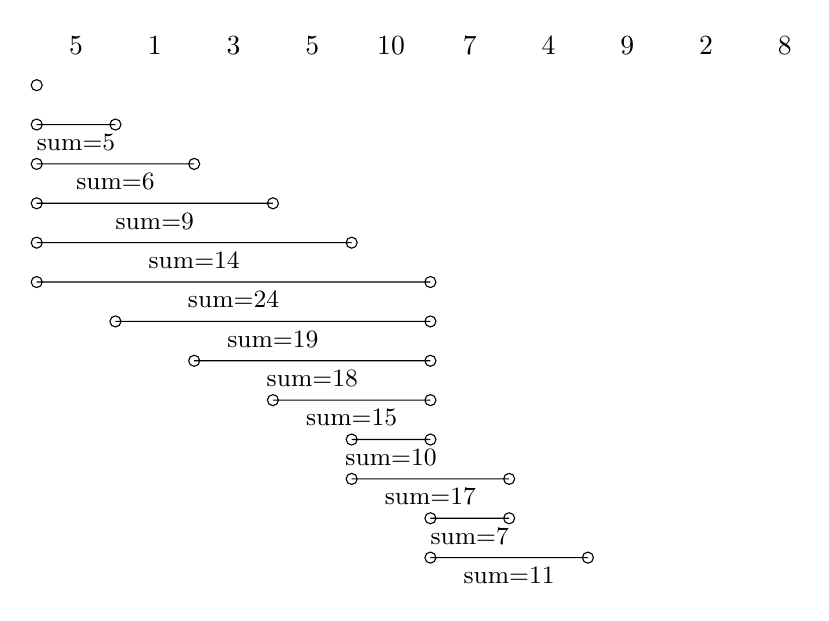
\begin{tikzpicture}
  \node at (0,0) {5};
  \node at (1,0) {1};
  \node at (2,0) {3};
  \node at (3,0) {5};
  \node at (4,0) {10};
  \node at (5,0) {7};
  \node at (6,0) {4};
  \node at (7,0) {9};
  \node at (8,0) {2};
  \node at (9,0) {8};

\draw (-0.5,-0.5) circle [radius=2pt,fill=black];
\draw (-0.5,-1.0) circle [radius=2pt,fill=black] -- node[below]
      {\small sum=5} (0.5,-1.0) circle [radius=2pt,fill=black];
\draw (-0.5,-1.5) circle [radius=2pt,fill=black] -- node[below] {\small sum=6} (1.5,-1.5) circle [radius=2pt,fill=black];
\draw (-0.5,-2) circle [radius=2pt,fill=black] -- node[below] {\small sum=9} (2.5,-2) circle [radius=2pt,fill=black];
\draw (-0.5,-2.5) circle [radius=2pt,fill=black] -- node[below] {\small sum=14} (3.5,-2.5) circle [radius=2pt,fill=black];
\draw (-0.5,-3) circle [radius=2pt,fill=black] -- node[below] {\small sum=24} (4.5,-3) circle [radius=2pt,fill=black];
\draw (0.5,-3.5) circle [radius=2pt,fill=black] -- node[below] {\small sum=19} (4.5,-3.5) circle [radius=2pt,fill=black];
\draw (1.5,-4) circle [radius=2pt,fill=black] -- node[below] {\small sum=18} (4.5,-4) circle [radius=2pt,fill=black];
\draw (2.5,-4.5) circle [radius=2pt,fill=black] -- node[below] {\small sum=15} (4.5,-4.5) circle [radius=2pt,fill=black];
\draw (3.5,-5) circle [radius=2pt,fill=black] -- node[below] {\small sum=10} (4.5,-5) circle [radius=2pt,fill=black];
\draw (3.5,-5.5) circle [radius=2pt,fill=black] -- node[below] {\small sum=17} (5.5,-5.5) circle [radius=2pt,fill=black];
\draw (4.5,-6) circle [radius=2pt,fill=black] -- node[below] {\small sum=7} (5.5,-6) circle [radius=2pt,fill=black];
\draw (4.5,-6.5) circle [radius=2pt,fill=black] -- node[below] {\small sum=11} (6.5,-6.5) circle [radius=2pt,fill=black];
\end{tikzpicture}
\end{center}

\begin{pbox}{Sum of Consecutive Prime Numbers}{Asian Regional 2005}
Find the number of ways a given integer can be expressed as the sum of consecutive prime numbers.

\aojid{1257}
\end{pbox}

First, find the prime numbers up to $10\,000$ using the Sieve of Eratosthenes (\pccbook{} page 112) or similar methods.
After that, it is the same as "Subsequence".
\subsection{Priority Queues}\label{section:priority-queue}
A priority queue (\eindex{priority queue}, \pccbook[p.~32]) is a data structure that allows data to be stored and retrieved, where the largest element among those not yet retrieved is retrieved first.

\begin{psbox}{Priority Queue}{AOJ}
Create a priority queue that can accept integers as input and retrieve them in descending order.

\aojid{ALDS1_9_C}
\end{psbox}

First, it is good to confirm that you can get accepted using the standard library \texttt{priority\_queue}\footnote{\url{http://en.cppreference.com/w/cpp/container/priority_queue}}.
If you implement a priority queue yourself, it is convenient to create a binary heap on an array or \texttt{vector}. See \pcaojbook[Chapter 10, pp.~232--] for details.

\begin{cbox}[emph={queue,priority\_queue,push,top,pop}]
\begin{verbatim}
#include <queue>
#include <iostream>
using namespace std;
int main() {
    priority_queue<int> Q; // Priority queue to store ints
    Q.push(3); // Add
    Q.push(4);
    Q.push(1);
    while (! Q.empty()) { // While there are elements
	int n = Q.top(); // Copy the first element
	Q.pop(); // Discard the first element
	cout << n << endl; // Displays 4, 3, 1 in that order
    }
}
\end{verbatim}
\end{cbox}

Since Python has a \texttt{heapq} package, we will use that.
\begin{pybox}
\begin{verbatim}
import heapq

Q = []
heapq.heappush(Q, 3)
heapq.heappush(Q, 4)
heapq.heappush(Q, 1)
while len(Q) > 0:
    n = heapq.heappop(Q)
    print(n)                    # Displays 1, 3, 4 in that order
\end{verbatim}
\end{pybox}
\section{Strings: Substrings, Concatenation, and Reversal}
In C++, you can obtain substrings of \texttt{string}\footnote{\url{http://en.cppreference.com/w/cpp/string/basic_string}} data using the \texttt{substr} method\footnote{\url{http://en.cppreference.com/w/cpp/string/basic_string/substr}}.
\begin{cbox}
  string word = "hello";
  for (size_t i=0; i<=word.size(); ++i) { // size() is the length of the string
    string l = word.substr(0,i);// String to the left of the i-th character
    string r = word.substr(i); // String from the i-th character onwards
    cout << l << ' ' << r << endl;
  }
\end{cbox}

Example output:\\
\begin{alltt}
 hello
h ello
he llo
hel lo
hell o
hello 
\end{alltt}

Exercise: Try changing \texttt{string word = "hello";} to a different word and running it.

\begin{pybox}
word = "hello";
for i in range(len(word)+1):
    l = word[0:i]
    r = word[i:]
    print(l+' '+r)  
\end{pybox}

For concatenation, use the \texttt{+} operator. It's the same in both C++ and Ruby.

\begin{cbox}
    string a = "AAA";
    string b = "BBB";
    string c = a+b; // Concatenation
    cout << c << endl; // AAABBB
\end{cbox}

For reversal, use the \texttt{reverse} function. The range is specified by \texttt{word.begin()} and \texttt{word.end()}. Using a notation similar to arrays, you can also write \texttt{reverse(\&word[0], \&word[0]+word.size());}.
 
\begin{cbox}
#include <algorithm>
    string word = "hello";
    reverse(word.begin(), word.end());
    cout << word << endl;  
\end{cbox}

\section{Sets}

In C++, the standard library provides the data structures \texttt{set}\footnote{\url{http://en.cppreference.com/w/cpp/container/set}} and \texttt{unordered\_set}\footnote{\url{http://en.cppreference.com/w/cpp/container/unordered_set}} (from C++11 onwards) to represent sets.
First, let's introduce an example of a set of integers.
Both provide almost the same operations, but here we will use insertion (\texttt{insert}), the total number of elements (\texttt{size}), and searching for the presence of a specified element (\texttt{count}).

In the implementation, \texttt{set} manages data with ordering, while \texttt{unordered\_set} manages data ignoring the order. The former is usually implemented with a binary search tree, and insertion and search require $O(\log N)$ time. That is, note that one operation becomes slower as the number of data $N$ increases. The latter is usually implemented using a hash table, and each operation is expected to take constant time on average.

\begin{cbox}[emph={set}]
\begin{verbatim}
#include <set>
    typedef set<int> set_t;
    set_t A;
    cout << A.size() << endl; // 0 because it is empty at first
    cout << A.count(3) << endl; // 0 because 3 is not included
    A.insert(1);
    A.insert(3);
    A.insert(5);
    A.insert(3);
    cout << A.size() << endl; // 3 for 1, 3, and 5
    cout << A.count(3) << endl; // 1 (at most 1 in the case of set)
    cout << A.count(4) << endl; // 0
\end{verbatim}
\end{cbox}

A set of strings can be used similarly.

\begin{cbox}[emph={set,string}]
\begin{verbatim}
#include <set>
#include <string>
    typedef set<string> set_t;
    set_t A;
    cout << A.size() << endl; // 0 because it is empty at first
    cout << A.count("hello") << endl; // 0 because "hello" is not included
    A.insert("hello");
    A.insert("world");
    A.insert("good morning");
    A.insert("world");
    cout << A.size() << endl; // "hello", "good morning", "world"
    cout << A.count("world") << endl; // 1 (at most 1 in the case of set)
    cout << A.count("hello!!!") << endl; // 0
\end{verbatim}
\end{cbox}

In Python, \texttt{set} is provided.\footnote{\url{https://docs.python.jp/3/library/stdtypes.html\#set}}
\begin{pybox}
\begin{verbatim}
s = set()
print('a' in s)                 # False
s.add('a')
print('a' in s)                 # True
s.discard('a')
print('a' in s)                 # False
\end{verbatim}
\end{pybox}

\begin{psbox}{Search - Dictionary}{AOJ}
Determine whether a word is in the dictionary.

\aojid{ALDS1_4_C}
\end{psbox}

\begin{tipsbox}{Time Limit Exceeded?}
If you do not get AC with a "Time Limit Exceeded (TLE)" verdict, it means that the execution time exceeded the allowable range.
If you are using \texttt{set} in C++, try using \texttt{unordered\_set}. In that case, select C++11 instead of C++ in the submission window.
\end{tipsbox}
\subsection{Bitsets}
As a special case of sets, when dealing with sets of integers from 0 to N, using a bit representation is efficient. In C++, the \texttt{bitset} type is provided as standard.

\begin{cbox}
\begin{verbatim}
#include <bitset>
#include <cassert>
std::bitset<128> a, b, c;
a[3] = 1; // Set the specified bit to on
b[5] = 1;
c = a | b; // Union of sets
\end{verbatim}
\end{cbox}
\section{Associative Arrays (map)}

When managing names associated with personal identification numbers, using an array is common.

\begin{cbox}
\begin{verbatim}
string name[30];
name[0] = "kaneko";
name[1] = "fukuda";
\end{verbatim}
\end{cbox}

However, how can we manage personal identification numbers associated with names?

\begin{cbox}
\begin{verbatim}
number["kaneko"] = 0; // We want to write like this
\end{verbatim}
\end{cbox}

An associative array is an abstract data type that manages \texttt{value}s associated with \texttt{key}s, providing the functionality described above. In C++, \texttt{map}\footnote{\url{http://en.cppreference.com/w/cpp/container/map}} and \texttt{unordered\_map}\footnote{\url{http://en.cppreference.com/w/cpp/container/unordered_map}} are provided, and in Python, \texttt{dict}\footnote{\url{https://docs.python.jp/3/library/stdtypes.html\#dict}} is available as standard.

\subsection{Maps}
In C++, the standard library provides the data structures \texttt{map} and \texttt{unordered\_map} (from C++11 onwards) to represent associative arrays.
First, let's introduce an example of a map from strings to integers.
Both provide almost the same operations, but here we will use insertion (using \texttt{[]}), the total number of elements (\texttt{size}), and searching for the presence of a specified key (\texttt{count}).

In the implementation, \texttt{map} manages data with ordering, while \texttt{unordered\_map} manages data ignoring the order. The former is usually implemented with a binary search tree, and insertion and search require $O(\log N)$ time. That is, note that one operation becomes slower as the number of data $N$ increases. The latter is usually implemented using a hash table, and each operation is expected to take constant time on average.

\begin{cbox}[emph={map}]
\begin{verbatim}
#include <map>
#include <string>
#include <iostream>
using namespace std;
int main() {
    map<string, int> A;
    cout << A.size() << endl; // 0 because it is empty at first
    cout << A.count("hello") << endl; // 0 because "hello" is not included
    A["hello"] = 1;
    A["world"] = 3;
    A["good morning"] = 5;
    A["world"] = 7;
    cout << A.size() << endl; // 3 for "hello", "good morning", and "world"
    cout << A.count("world") << endl; // 1 (at most 1 in the case of map)
    cout << A["world"] << endl; // 7
    cout << A.count("hello!!!") << endl; // 0
}
\end{verbatim}
\end{cbox}

In Python, \texttt{dict} is provided.\footnote{\url{https://docs.python.jp/3/library/stdtypes.html\#dict}}
\begin{pybox}
\begin{verbatim}
d = {}
print('a' in d)                 # False
d['a'] = 1
print('a' in d)                 # True
print(d['a'])                  # 1
del d['a']
print('a' in d)                 # False
\end{verbatim}
\end{pybox}

\begin{psbox}{Search - Frequency}{AOJ}
Count the frequency of each word.

\aojid{ALDS1_4_B}
\end{psbox}

\begin{tipsbox}{Time Limit Exceeded?}
If you do not get AC with a "Time Limit Exceeded (TLE)" verdict, it means that the execution time exceeded the allowable range.
If you are using \texttt{map} in C++, try using \texttt{unordered\_map}. In that case, select C++11 instead of C++ in the submission window.
\end{tipsbox}

\begin{pbox}{The Number of Palindromes}{Mock National Preliminary 2008}
Find the number of palindromic substrings in a given string.

\aojid{2018}
\end{pbox}

Hint:
\begin{itemize}
\item A palindrome is a string that reads the same forwards and backward.
\item If the string is long, it is not possible to check all substrings.
\item If the string is short, it is possible to check all substrings.
\item If the string is a palindrome, the string with the first and last characters removed is also a palindrome.
\end{itemize}

\begin{pbox}{The Number of Different Substrings}{Mock National Preliminary 2008}
Find the number of different substrings in a given string.

\aojid{2017}
\end{pbox}

Hint:
\begin{itemize}
\item If the string is long, it is not possible to check all substrings.
\item If the string is short, it is possible to check all substrings.
\item If the string is a substring, the string with the last character removed is also a substring.
\end{itemize}

\begin{pbox}{The Number of Different Subsequences}{Mock National Preliminary 2008}
Find the number of different subsequences in a given string.

\aojid{2016}
\end{pbox}

Hint:
\begin{itemize}
\item If the string is long, it is not possible to check all subsequences.
\item If the string is short, it is possible to check all subsequences.
\item If the string is a subsequence, the string with the last character removed is also a subsequence.
\end{itemize}

\begin{pbox}{The Number of Different Substrings}{Mock National Preliminary 2008}
Find the number of different substrings in a given string.

\aojid{2017}
\end{pbox}

Hint:
\begin{itemize}
\item If the string is long, it is not possible to check all substrings.
\item If the string is short, it is possible to check all substrings.
\item If the string is a substring, the string with the last character removed is also a substring.
\end{itemize}

\begin{pbox}{The Number of Different Subsequences}{Mock National Preliminary 2008}
Find the number of different subsequences in a given string.

\aojid{2016}
\end{pbox}

Hint:
\begin{itemize}
\item If the string is long, it is not possible to check all subsequences.
\item If the string is short, it is possible to check all subsequences.
\item If the string is a subsequence, the string with the last character removed is also a subsequence.
\end{itemize}
\section{Exercises}

\begin{pbox}{Queue}{AOJ}
Implement a queue using two stacks.

\aojid{ALDS1_3_C}
\end{pbox}

\begin{pbox}{Parenthesis Matching}{AOJ}
Determine whether parentheses are correctly matched.

\aojid{ALDS1_3_C}
\end{pbox}

\begin{pbox}{Area of a Polygon}{AOJ}
Find the area of a polygon.

\aojid{CGL_3_A}
\end{pbox}

\begin{pbox}{Convex Hull}{AOJ}
Find the convex hull of a set of points.

\aojid{CGL_4_A}
\end{pbox}

\begin{pbox}{Minimum Enclosing Circle}{AOJ}
Find the minimum enclosing circle of a set of points.

\aojid{CGL_7_A}
\end{pbox}

\begin{pbox}{The Number of Different Substrings}{Mock National Preliminary 2008}
Find the number of different substrings in a given string.

\aojid{2017}
\end{pbox}

\begin{pbox}{The Number of Different Subsequences}{Mock National Preliminary 2008}
Find the number of different subsequences in a given string.

\aojid{2016}
\end{pbox}

\begin{pbox}{The Number of Palindromes}{Mock National Preliminary 2008}
Find the number of palindromic substrings in a given string.

\aojid{2018}
\end{pbox}

\begin{pbox}{The Number of Palindromes}{Mock National Preliminary 2008}
Find the number of palindromic substrings in a given string.

\aojid{2018}
\end{pbox}

\begin{pbox}{The Number of Different Substrings}{Mock National Preliminary 2008}
Find the number of different substrings in a given string.

\aojid{2017}
\end{pbox}

\begin{pbox}{The Number of Different Subsequences}{Mock National Preliminary 2008}
Find the number of different subsequences in a given string.

\aojid{2016}
\end{pbox}

\subsection{Mapping Strings to Numbers}

\begin{cbox}[emph={map}]
\begin{verbatim}
#include <iostream>
#include <string>
#include <map>
using namespace std;
int main() {
  map<string,int> table; // Map to associate strings with numbers
  table["taro"] = 180;
  table["hanako"] = 160;
  cout << table["taro"] << endl; // 180
  cout << table["ichirou"] << endl; // 0
}  
\end{verbatim}
\end{cbox}

In this example, the \texttt{key} is a string, and the \texttt{value} is an integer.

\begin{pybox}
\begin{verbatim}
all = {}
print(len(all))                 # 0
all["hello"] = 1
all["world"] = 100
all["good morning"] = 20
print(len(all))                 # 3
for k,v in sorted(all.items()):
    print(k,v)
# good morning 20
# hello 1
# world 100
\end{verbatim}
\end{pybox}

\begin{psbox}{English Sentence}{PC Koshien 2004}
Given a string, output the most frequent word and the word with the most characters.

\aojid{0029}
\end{psbox}


The length of a string \texttt{s} of type \texttt{string} can be obtained with \texttt{s.size()}.
\subsection{Counting String Occurrences}

The behavior when a \texttt{key} does not exist depends on the processing system and settings, but in the above example, it is used so that it becomes 0.
This makes it easy to count the number of occurrences.

\begin{cbox}
  table["ichirou"]+=1;
  cout << table["ichirou"] << endl; // 1
  table["ichirou"]+=1;
  cout << table["ichirou"] << endl; // 2
\end{cbox}

\begin{pybox}
\begin{verbatim}
# Using a regular hash
table = {}  
# table["ichirou"] += 1 ... ng!
table["ichirou"] = table.get("ichirou", 0) + 1
if not "world" in table:
   table["world"] = 1
# Using Counter
import collections
c = collections.Counter()
c["ichirou"] += 1 # ok
\end{verbatim}
\end{pybox}
\subsection{Listing Elements of Associative Arrays}

\begin{c11box}[emph={map,iterator,begin,end,first,second}]
\begin{verbatim}
#include <iostream>
#include <map>
#include <string>
using namespace std;
int main() {
  map<string,int> phone;
  phone["taro"] = 123;
  phone["jiro"] = 456;
  phone["saburo"] = 789;

  for (auto p=phone.begin(); // Equivalent to i=0
       p!=phone.end(); // Equivalent to i<N
       ++p) {
      cout << p->first << " " << p->second << endl;
  }
// The output order is
// jiro 456
// saburo 789
// taro 123
}
\end{verbatim}
\end{c11box}

The parts written in \textcolor{red}{red} are boilerplate, and since they are difficult to grasp at first glance, please use them as is. In the case of arrays, an integer \texttt{i} is used as an index, but in the case of associative arrays, because there is complex processing, an abstract interface called an iterator is used instead of an integer.\footnote{Here, we used the C++11 feature and wrote \texttt{auto}. The actual type is \texttt{map<string,int>::iterator}.} Also, for the initial and end values, \texttt{begin()} and \texttt{end()} are used instead of $0$ and $N$. Inside the loop, the \texttt{key} of each element is referenced by \texttt{p->first}, and the \texttt{value} is referenced by \texttt{p->second}.
\section{Exercises}
\begin{pbox}{Organize Your Train part II}{National Preliminary 2006}
How many ways are there to rearrange a freight train?

\aojid{1142}
\end{pbox}

\begin{cbox}
int M;
string S;
int main() {
    cin >> M;
    for (int i=0; i<M; ++i) {
        cin >> S;
        std::set<std::string> all; // Set of strings
        all.insert(S); // Insert S into all
        for (size_t i=1; i<S.size(); ++i) {
            std::string L = S.substr(0,i); // Set L to the [0,i) characters of S
            std::string R = S.substr(i); // Set R to the [i,S.length()) characters of S
            std::string L2, R2;
            std::reverse(L.begin(), L.end()); // Set L2 to the reverse of L
            std::reverse(R.begin(), R.end()); // Set R2 to the reverse of R
            all.insert(R+L); // Insert R+L into all
            all.insert(R2+L); // Insert R2+L into all
            all.insert(L+R2); // Insert L+R2 into all
            all.insert(R2+L2); // Insert R2+L2 into all
            all.insert(L2+R); // Insert L2+R into all
            all.insert(L2+R2); // Insert L2+R2 into all
        }
        cout << all.size() << endl; // Output the number of elements in all (all.size())
    }
}  
\end{cbox}

\begin{pbox}{Era Name}{Mock Regional Preliminary 2010}
Given the correspondence between (fictitious) Western years and (fictitious) era names, organize and memorize them.
Then, when a Western year is given as a question, if the era name is known, answer with the era name; otherwise, answer with ``Unknown''.

\aojid{2242}
\end{pbox}

Problem Supplement: In the input example, "showa 62 1987" represents two pieces of information:
\begin{itemize}
\setlength{\itemsep}{0pt}
\item The Western year of the first year of Showa (year 1) is 1926.
\item Showa continued (at least) until 1987.
\end{itemize}
Without other information, it is not known whether 1988 is Showa (another era name might be used between Showa and Heisei), so answer with ``Unknown''.

Example Answer: Record each piece of information by dividing it into two: a correspondence table of Western years and the era name for which that year is year 1, and a table of how many years each era name lasted at most.
Use \texttt{map<int,string>} for the former and \texttt{map<string,int>} for the latter.
\subsection{Managing Intervals}

\begin{pbox}{Restrictive Filesystem$\star$}{Mock National Preliminary 2009}
Implement read, write, and delete operations in a simple file system, and output the data read at each point in time.

\aojid{2152}
\end{pbox}

Example Solution: \textcolor{white}{Represent the state of the disk using an associative array \texttt{map<pair<int,int>, int>} that maps intervals \texttt{pair<int,int>} to file IDs, and simulate the read, write, and delete operations.}
\subsection{Applications of Sets}

\begin{pbox}{Twenty Questions$\star$}{Asian Regional 2009}
Consider the best way to ask questions to distinguish each object. The next question can be changed depending on the answer.

\aojid{1302}
\end{pbox}

\begin{pbox}{Sweets$\star$}{Algorithmic Engagements 2010}
There are $n \le 24$ positive numbers. Divide them among three siblings $A, D, B$. Among the ways of dividing them that satisfy $A \ge D \ge B$, find the division that minimizes $A-B$.

\url{https://szkopul.edu.pl/problemset/problem/cEMM4bdcKN06uikzs9BRSqkz/site/}
\end{pbox}

Even the solution that the person in charge implemented, which is supposed to be the explained solution, gets TLE (time limit exceeded) (about 5 seconds for the maximum case), so it seems better to download the data from ``Useful Resources'' and not worry about the time if it is correct.

\begin{pbox}{Building Blocks$\star$}{15th Polish Olympiad in Informatics}
There are $N$ bar graphs. Select some consecutive $K (\le N)$ bars and align them to the same height.
Increasing or decreasing the height by 1 incurs the same cost. Output the minimum total cost and the height of each bar graph at that time.

\url{https://szkopul.edu.pl/problemset/problem/KC7c6nYfAXCbCGszqhIeOGxP/site/}
\end{pbox}

It is okay to use \texttt{cin} instead of \texttt{scanf} for input/output. It can be solved by combining STL data structures.

\chapter{Graphs (1) Spanning Trees}

\begin{itembox}[l]{Overview}
Starting today, we will discuss graphs over several sessions. Graphs are a fundamental concept for modeling various situations and problems.
This week, let's find the minimum spanning tree. Also, as a tool for that, we will introduce a data structure called Disjoint Set (Union-Find Tree) for managing groups.
\end{itembox}
\section{Graphs and Trees}

Graphs are often used when modeling the world with a focus on relationships.
Examples include route maps, logistics, and family relationships.
(\pccbook[Sections 2-5, p.~87] "Everything is actually a graph")

\begin{center}
      \begin{tikzpicture}[node distance=15mm]
        \node[city] (A)              {$a$};
        \node[city] (B) [below of=A] {$b$};
        \node[city] (C) [below of=B] {$c$};
        \node[city] (D) [right of=B] {$d$};
        \path[thick] (A) edge (B);
        \path[thick] (B) edge (C);
        \path[thick] (C) edge (D);
        \path[thick] (D) edge (B);
      \end{tikzpicture}
\end{center}
\subsection{Graph Terminology}

A \jindex{graph}{graph} consists of \jindex{vertices}{vertices} (also called nodes or points, \eindex{vertex}; plural is vertices) and \jindex{edges}{edges} (also called branches, lines, \eindex{edge}, \eindex{arc}).
A graph $G$ is represented by a set of vertices $V$ and a set of edges $E$ as $G=(V,E)$.

Example: A graph with three vertices $V=\{1,2,3\}$ where all vertices are connected (a triangle) has edges $E=\{\{1,2\},\{2,3\}, \{3,1\}\}$.

When a vertex $v$ and an edge $e$ satisfy $v\in e$, we say that $v$ is \textbf{incident} to $e$.
For a vertex $v$, the number of incident edges $|E(v)|$ is called the \jindex{degree}{degree} (\eindex{degree}) of $v$.
Two vertices are said to be \textbf{adjacent} if they share a common incident edge.
A sequence of adjacent vertices is called a \jindex{path}{path} (\eindex{path}, trail, walk have slightly different meanings when studied in detail, so be careful when learning more).

Example: The degree of each vertex in a triangle is 2.

\subsection{Trees}

A special type of graph (connected and without cycles) is called a \textbf{tree}. Trees are easier to handle than general graphs.
Examples of things that can be represented by trees include expressions (3 + (5 - 2)), hierarchical file systems (excluding links, etc.), family trees representing one's ancestors (when there are no marriages between relatives such as cousins), and Internet domain names.

\begin{center}
  \begin{tabular}{c@{\hspace{3em}}cc}
\imagetop{\begin{forest}
  ctree [ a ]
    \end{forest}}
&
\imagetop{\begin{forest}
  ctree [ a [ b ] [ c ] [ d ] ]
    \end{forest}}
&
\imagetop{\begin{forest}
  ctree [ a [b] [ c [ d] [e]]]
    \end{forest}}
\\
Tree 1 & Tree 2 & Tree 3
  \end{tabular}
\end{center}

\paragraph{Definitions}

For an undirected graph $G$, $G$ is called \textbf{connected} if there exists a $v-w$ path for all pairs of vertices $v,w$.
A graph that does not contain cycles is called a \jindex{forest}{forest}.
A connected forest is called a \jindex{tree}{tree}.

If the number of vertices in a graph $T$ is $n$, then $T$ being a tree is equivalent to the following:
\begin{itemize}
\item $T$ consists of $n-1$ edges and has no cycles.
\item $T$ consists of $n-1$ edges and is connected.
\item For any two vertices in $T$, there exists only one path connecting the two vertices.
\item $T$ is connected, and for any edge in $T$, the graph obtained by removing that edge from $T$ is disconnected.
\item $T$ contains no cycles, and for any two non-adjacent vertices $x$ and $y$, the graph obtained by adding an edge connecting $x$ and $y$ to $T$ contains a cycle.
\end{itemize}

A special vertex in a tree is called the \jindex{root}{root}.
When visualizing a graph, the root is often placed at the top or bottom. A vertex with a degree of 1 is called a \jindex{leaf}{leaf}.
For two vertices connected by an edge in a tree, the vertex closer to the root (or the root itself) is called the \jindex{parent}{parent}, and the vertex farther away is called the \jindex{child}{child}.
\subsection{Tree Representation Focusing on "Parents"}

One way to represent a "tree" with $N$ nodes on a computer is to assign numbers from 1 to $N$ to each node and manage the parent of each node using a one-dimensional array (hereinafter denoted as \texttt{P[]}, using the initial of parent). Trees have the property that they have at most one parent. Therefore, for the value of \texttt{P[i]} corresponding to node $i$, we assign the parent's number if node $i$ has a parent, and a special number such as $-1$ or itself if it does not have a parent (i.e., it is the \textbf{root}).

Note that in general graphs that are not trees, each node can have multiple children, so when managing children, a more complex representation than a one-dimensional array (such as an adjacency list or adjacency matrix, see Section~\ref{section:adjacency-matrix}) is required.

\begin{center}
  \begin{tabular}{lc@{\hspace{3em}}cc}
Tree&
\imagetop{\begin{forest}
  ctree [ 1 ]
    \end{forest}}
&
\imagetop{\begin{forest}
  ctree [ 1 [2][3][4] ]
    \end{forest}}
&   
\imagetop{\begin{forest}
  ctree [ 5 [2][3[4][1]] ]
    \end{forest}}
\\
Array Representation&
\begin{tabular}{c|c}
i & 1 \\
P[i] & 1
\end{tabular}
&
\begin{tabular}{c|cccc}
i & 1 & 2 & 3 & 4\\
P[i] & 1 & 1 & 1 & 1
\end{tabular}
&
\begin{tabular}{c|ccccc}
i & 1 & 2 & 3 & 4 & 5\\
P[i] & 3 & 5 & 5 & 3 & 5
\end{tabular}
  \end{tabular}
\end{center}
\section{Disjoint Set (Union-Find Tree)}
One efficient method for determining whether two elements belong to the same group is the \jindex{Union Find}{Union Find} tree (\pcaojbook[pp.~318--], \pccbook[pp.~81--]). It is also called a \jindex{Disjoint-set}{Disjoint-set} data structure.
It allows for the merging of groups but not their separation (c.f. link-cut tree).

\begin{center}
  \begin{forest}
    [,rootempty [1] [2] [3 [4]] [5 [6] [7 [8 [9]]]]]
  \end{forest}
\\
\begin{tabular}{c|ccccccccc}
   i & 1 & 2 & 3 & 4 & 5 & 6 & 7 & 8 & 9\\
P[i] & 1 & 2 & 3 & 3 & 5 & 5 & 5 & 7 & 8
\end{tabular}\\
Four groups: $\{1\}, \{2\}, \{3,4\}, \{5,6,7,8,9\}$
\end{center}

\paragraph{Determination}
If elements belong to the same tree, they are in the same group; otherwise, they are in different groups.
This is determined by checking the root.
Example:
\begin{itemize}
\setlength{\itemsep}{0pt}
\item \textbf{Q1. Do 6 and 8 belong to the same group?}\\
The root of the tree to which 6 belongs is 5, and similarly, the root of 8 is 5 \dingright{} Same group.
\item \textbf{Q2. Do 2 and 4 belong to the same group?}\\
The root of the tree to which 2 belongs is 2, and the root of 4 is 3 \dingright{} Different groups.
\end{itemize}
 
\paragraph{Merging}

Merging is the operation of combining two nodes into the same group. This is achieved by connecting the root of the tree to which one node belongs to the root of the tree to which the other node belongs.
It does not matter which root is connected to which. (It is more efficient to attach the smaller (lower) tree under the larger (higher) tree, but this is omitted in this material.)

\begin{center}
  \begin{tabular}{c@{\hspace{2em}}c}\hline
\imagetop{\begin{forest}
     [,rootempty [1] [2]]
  \end{forest}}
&
\imagetop{\begin{forest}
ctree [1 [2]]
  \end{forest}}
\\
\begin{tabular}{c|cc}
   i & 1 & 2\\
P[i] & 1 & 2
\end{tabular}
&
\begin{tabular}{c|cc}
   i & 1 & 2\\
P[i] & 1 & \cemph{1}\end{tabular}
\\
Original graph & Graph after merging 1 and 2\\\hline

\\
\imagetop{\begin{forest}
    [,rootempty,for tree={s sep=10mm} [3 [4,rtree]] [5 [6] [7 [8,rtree [9,ctree]]]]]
  \end{forest}}
&
\imagetop{\begin{forest}
ctree [5,for tree={s sep=10mm}, [3 [4]] [6] [7 [8 [9]]]]
  \end{forest}}
\\
\begin{tabular}{c|ccccccc}
   i & 3 & 4 & 5 & 6 & 7 & 8 & 9\\
P[i] & 3 & 3 & 5 & 5 & 5 & 7 & 8
\end{tabular}
&
\begin{tabular}{c|ccccccc}
   i & 3 & 4 & 5 & 6 & 7 & 8 & 9\\
P[i] & \cemph{5} & 3 & 5 & 5 & 5 & 7 & 8
\end{tabular}
\\
Original graph & Graph after merging 4 and 8\\
&(To merge the entire groups, connect the roots)\\\hline
  \end{tabular}
\end{center}


\paragraph{Optimization: Path Compression}

The operation of finding the root of a node takes longer as the distance from the root increases.
Therefore, once the root is found, it is effective to improve efficiency by reconnecting the related nodes to directly connect to the root as much as possible.

\begin{tabular}{c@{\hspace{5em}}c}
\imagetop{\begin{forest}
ctree [5 [3 [4]] [6] [7 [8[9,rtree]]]]
  \end{forest}}
&
\imagetop{\begin{forest}
ctree [5 [3 [4]] [6] [7,rtree] [8,rtree][9,rtree]]
  \end{forest}}
\\
\begin{tabular}{c|ccccccc}
   i & 3 & 4 & 5 & 6 & 7 & 8 & 9\\
P[i] & 5 & 3 & 5 & 5 & 5 & 7 & 8
\end{tabular}
&
\begin{tabular}{c|ccccccc}
   i & 3 & 4 & 5 & 6 & 7 & 8 & 9\\
P[i] & 5 & 3 & 5 & 5 & \cemph{5} & \cemph{5} & \cemph{5}
\end{tabular}
\\
Original graph & Deform the tree while finding root(9) = 5
\end{tabular}

\paragraph{Code Example:}
Below are code examples for initialization, determination, and merging. If it is difficult to understand the code at first glance, it is good to try writing it out and testing its operation before trying to understand it again. (The concept of \texttt{rank} is ignored.)

\begin{cbox}[emph={root,is\_same\_set,unite}]
\begin{verbatim}
int P[10010]; // Can handle vertices from 0 to 10000
void init(int N) { // Initialization: Initially, all vertices are separate
    for (int i=0; i<N; ++i) P[i] = i;
}
int root(int a) { // Find the root (representative element) of a
    if (P[a] == a) return a; // a is the root
    return (P[a] = root(P[a])); // Find the root of a's parent and set it as a's parent
}
bool is_same_set(int a, int b) { // Do a and b belong to the same group?
    return root(a) == root(b);
}
void unite(int a, int b) { // Combine a and b into the same group
    P[root(a)] = root(b);
}
\end{verbatim}
\end{cbox}
The part where \texttt{P[a]} is assigned at the end of the \texttt{root} function is the path compression.

\begin{pybox}[emph={root,is\_same\_set,unite}]
\begin{verbatim}
P = [i for i in range(N)]
def root(x):
    path_to_root = []
    while P[x] != x:
        path_to_root.append(x)
        x = P[x]
    for node in path_to_root:
        P[node] = x  # Path compression
    return x
def is_same_set(x,y):
    return root(x) == root(y)
def unite(x,y):
    P[root(x)] = root(y)
\end{verbatim}
\end{pybox}
In Python, the recursion depth limit is stricter than in C++, so the \texttt{root} function is implemented with a \texttt{while} loop instead of recursion.


Execution example:

\begin{cbox}
\begin{verbatim}
int main() {
  init(100);
  cout << is_same_set(1, 3) << endl;
  unite(1,2);
  cout << is_same_set(1, 3) << endl;
  unite(2,3);
  cout << is_same_set(1, 3) << endl;
}
\end{verbatim}
\end{cbox}

\begin{psbox}{Disjoint Set: Union Find Tree}{AOJ}
Manage groups with Disjoint Set.

Note: Ignore the indices of the sets $S_1,\ldots,S_k$. In particular, it does not correspond to $S_x$ in "the set $S_x$ containing $x$".

\aojid{DSL_1_A}
\end{psbox}
\section{Spanning Trees}

A tree formed using all the vertices of a connected graph $G$ and all or a subset of its edges is called a \jindex{spanning tree}{spanning tree} or a \textbf{full-vertex tree}.
When the edges have weights, a tree where the sum of the weights of the edges included in the spanning tree is minimal is called a \jindex{minimum (weight) spanning tree}{minimum spanning tree}.

Note: If a graph is connected, a spanning tree exists. A spanning tree is not necessarily unique (in the case of a complete graph, there are $n^{n-2}$ of them). A minimum spanning tree is also not necessarily unique. The problem of finding a minimum spanning tree often refers to the problem of finding one of the minimum spanning trees.

\begin{center}
  \begin{tabular}{c@{\hspace{2em}}c@{\hspace{2em}}c@{\hspace{2em}}c}
      \begin{tikzpicture}[node distance=15mm]
        \node[city] (A)              {$a$};
        \node[city] (D) [right of=A] {$d$};
        \node[city] (B) [below of=A] {$b$};
        \node[city] (C) [right of=B] {$c$};
        \path[thick] (A) edge (B);
        \path[thick] (B) edge (C);
        \path[thick] (C) edge (A);
        \path[thick] (C) edge (D);
        \path[thick] (D) edge (A);
      \end{tikzpicture}
&
      \begin{tikzpicture}[node distance=15mm]
        \node[city] (A)              {$a$};
        \node[city] (D) [right of=A] {$d$};
        \node[city] (B) [below of=A] {$b$};
        \node[city] (C) [right of=B] {$c$};
        \path[ultra thick, draw=red] (A) edge (B);
        \path[thick] (B) edge (C);
        \path[thick] (C) edge (A);
        \path[ultra thick, draw=red] (C) edge (D);
        \path[ultra thick, draw=red] (D) edge (A);
      \end{tikzpicture}
&
      \begin{tikzpicture}[node distance=15mm]
        \node[city] (A)              {$a$};
        \node[city] (D) [right of=A] {$d$};
        \node[city] (B) [below of=A] {$b$};
        \node[city] (C) [right of=B] {$c$};
        \path[thick] (A) edge (B);
        \path[ultra thick, draw=red] (B) edge (C);
        \path[thick] (C) edge (A);
        \path[thick] (C) edge (D);
        \path[ultra thick, draw=red] (D) edge (A);
      \end{tikzpicture}
&
      \begin{tikzpicture}[node distance=15mm]
        \node[city] (A)              {$a$};
        \node[city] (D) [right of=A] {$d$};
        \node[city] (B) [below of=A] {$b$};
        \node[city] (C) [right of=B] {$c$};
        \path[thick] (A) edge (B);
        \path[ultra thick, draw=red] (B) edge (C);
        \path[ultra thick, draw=red] (C) edge (A);
        \path[ultra thick, draw=red] (C) edge (D);
        \path[ultra thick, draw=red] (D) edge (A);
      \end{tikzpicture}
\\
Original Graph &
Red Subgraph is a Spanning Tree & Not a Spanning Tree (Disconnected) & Not a Spanning Tree (Cycle)
  \end{tabular}
\end{center}
\subsection{Kruskal's Algorithm}

Among the well-known methods for finding the minimum spanning tree, there are Prim's algorithm and \jindex{Kruskal's algorithm}{Kruskal's algorithm} (\eindex{Kruskal}), but here we will introduce the latter.

Kruskal's algorithm operates as follows (\pccbook[pp.~101--]):
\begin{itemize}
\setlength{\itemsep}{0pt}
    \item Sort the edges in ascending order of weight (see Chapter \ref{section:sort-pairs} for how to sort pairs of numbers).
    \begin{itemize}
        \item Method 1: Sort $\langle$weight, start vertex, end vertex$\rangle$
        \item Method 2: Sort $\langle$weight, edge ID$\rangle$ and manage a separate array to associate IDs with start and end vertices.
    \end{itemize}
    \item Let $T$ be a forest in the process of being built (initially empty, a graph without cycles, not necessarily connected).
    \item For each edge $e$ in ascending order of weight, perform the following operation:
    If $T+e$ (the graph obtained by adding edge $e$ to graph $T$) does not contain a cycle, add $e$ to $T$.
\end{itemize}

\begin{center}
  \begin{tabular}{c@{\hspace{2em}}c@{\hspace{2em}}c@{\hspace{2em}}c}
      \begin{tikzpicture}[node distance=15mm]
        \node[city] (A)              {$a$};
        \node[city] (D) [right of=A] {$d$};
        \node[city] (B) [below of=A] {$b$};
        \node[city] (C) [right of=B] {$c$};
        \path[thick] (A) edge node [left] {4} (B);
        \path[thick] (B) edge node [below] {5} (C);
        \path[thick] (C) edge node [above] {3} (A);
        \path[thick] (C) edge node [right] {2} (D);
        \path[thick] (D) edge node [above] {1} (A);
      \end{tikzpicture}
&
      \begin{tikzpicture}[node distance=15mm]
        \node[city] (A)              {$a$};
        \node[city] (D) [right of=A] {$d$};
        \node[city] (B) [below of=A] {$b$};
        \node[city] (C) [right of=B] {$c$};
        \path[thick] (A) edge node [left] {4} (B);
        \path[thick] (B) edge node [below] {5} (C);
        \path[thick] (C) edge node [above] {3} (A);
        \path[thick] (C) edge node [right] {2} (D);
        \path[ultra thick, draw=ired] (D) edge node [above] {1} (A);
      \end{tikzpicture}
&
      \begin{tikzpicture}[node distance=15mm]
        \node[city] (A)              {$a$};
        \node[city] (D) [right of=A] {$d$};
        \node[city] (B) [below of=A] {$b$};
        \node[city] (C) [right of=B] {$c$};
        \path[thick] (A) edge node [left] {4} (B);
        \path[thick] (B) edge node [below] {5} (C);
        \path[thick] (C) edge node [above] {3} (A);
        \path[ultra thick, draw=ired] (C) edge node [right] {2} (D);
        \path[ultra thick, draw=ired] (D) edge node [above] {1} (A);
      \end{tikzpicture}
&
      \begin{tikzpicture}[node distance=15mm]
        \node[city] (A)              {$a$};
        \node[city] (D) [right of=A] {$d$};
        \node[city] (B) [below of=A] {$b$};
        \node[city] (C) [right of=B] {$c$};
        \path[ultra thick, draw=ired] (A) edge node [left] {4} (B);
        \path[thick] (B) edge node [below] {5} (C);
        \path[thick] (C) edge node [above] {3} (A);
        \path[ultra thick, draw=ired] (C) edge node [right] {2} (D);
        \path[ultra thick, draw=ired] (D) edge node [above] {1} (A);
      \end{tikzpicture}
\\
Original Graph &
Adopt edge ad (weight 1) & Adopt edge cd (weight 2) & Adopt edge ab (weight 4)
  \end{tabular}
\end{center}

One efficient method for determining whether $T+e$ contains a cycle is the union-find tree.
Within the above Kruskal's algorithm, each time an edge $e$ is added, the vertices at both ends of the edge are incorporated into the same group using \texttt{unite}.
If \texttt{is\_same\_set(a,b)} is true for the two ends $a,b$ of edge $e$, then adding edge $e$ will create a cycle (because there is a path between $a$ and $b$ other than $e$).

\begin{psbox}{Graph II - Minimum Spanning Tree}{AOJ}
Find the sum of the weights of the minimum spanning tree of a given graph.

\aojid{ALDS1_12_A}
\end{psbox}

\begin{pbox}{Stellar Performance of the Debunkey Family}{PC Koshien 2008}
Problem: Minimize the maintenance cost of bridges while keeping the city connected.

\aojid{0180}  
\end{pbox}

\paragraph{Input/Output Example}
The following code can be created, for example, to read the input and output the edges in order of increasing maintenance cost. It is okay to copy this as is, since the main focus today is on practicing Kruskal's algorithm.

\begin{cbox}
\begin{verbatim}
#include <algorithm>
int N, M, A[10010], B[10010], COST[10010];
pair<int,int> bridge[10010]; // Pair of cost and bridge number
int main() {
    while // (Read N and M, process if N is greater than 0) {
        for (int i=0; i<M; ++i) {
            // Read A[i], B[i], and COST[i];
            bridge[i].first = COST[i];
            bridge[i].second = i;
        }
        sort(bridge, bridge+M); // Sort in ascending order of cost
        for (int i=0; i<M; ++i) {
            int cost = bridge[i].first;
            int a = A[bridge[i].second];
            int b = B[bridge[i].second];
            // Display "a bridge with cost connects a to b"
        }
    }
}
\end{verbatim}
\end{cbox}

In the code, \texttt{pair<int,int>} is equivalent to \texttt{struct pair \{ int first, second; \};}.

\paragraph{Example Answer:} Assuming the above preparation is done, the outline of the answer is as follows.

\begin{cbox}
\begin{verbatim}
        int total = 0;
        for (int i=0; i<M; ++i) { // In order of cheapest bridge
            if // (If the nodes at both ends of the bridge are already connected)
                continue;
            // Merge the nodes at both ends of the bridge into the same group;
            // Add the cost of the bridge to the total;
        }
        // Output the total;
\end{verbatim}
\end{cbox}
\section{Exercises}

\begin{pbox}{Marked Ancestor}{Summer Camp 2009}
Find the nearest marked ancestor. Initially, only the root is marked.

Note: The total may exceed the range of int, so use long long.

  \aojid{2170}
\end{pbox}

Supplement: In the figure below, initially, the ``nearest marked ancestor'' of "cat" is "animal". If "mammal" is marked later, the ``nearest marked ancestor'' of "cat" becomes "mammal".

\begin{center}
\begin{forest}
ctree [animal [amphibian [frog]] [reptile] [mammal [cat][dog]]]
\end{forest}
\end{center}

\begin{tipsbox}{Hint}
First, read all the command sequences such as Mark and Query, and then, \textcolor{white}{if you process them by removing the marks from the back...?}
\end{tipsbox}
\subsection{Disjoint Sets}
\begin{pbox}{Fibonacci Sets}{Aizu University Programming Contest 2003}
Let $f[i]$ denote the $i$-th Fibonacci number. For some $i, j$ ($1\le i,j \le V$), if the absolute difference between $f[i]\%1001$ and $f[j]\%1001$ is less than $d$, then nodes $i$ and $j$ belong to the same group. Given $V$ and $d$, count the number of groups.

\aojid{1016}
\end{pbox}

Example solution:
\begin{cbox}
int F[1001];
int main() {
    F[0] = 1, F[1] = 2;
    // ... Pre-calculate and assign the i-th Fibonacci number % 1001 to F[i]
    while (cin >> V >> D) {
        // Initialize the tree
        for (int i=1; i<=V; ++i)
            for (int j=i+1; j<=V; ++j)
                if // (If the absolute difference between F[j] and F[i] is less than D)
                    // Unite group i and group j;
        // Count and output the number of i in [1,V] such that root(i) == i
    }
}  
\end{cbox}

Create and test in detail:
\begin{itemize}
\setlength{\itemsep}{0pt}
\item Calculation of Fibonacci numbers: Assign values to F[2]..F[1000] using a for loop (using \texttt{F} instead of \texttt{a[2]} in approach 3 of Section~\ref{section:fibonacci}, and taking the remainder of 1001 during the calculation is the difference).
That is, if you increase $i$ from the smallest, you can calculate \texttt{F[i] = F[i-2]+F[i-1];} as defined. Take the remainder of 1001 even during the calculation to prevent overflow.
(Display and confirm)
\item Create a Union-find tree: Basically as in the material\\
(Initialize, display the tree and confirm. Merge a few and display the tree to confirm.)
\item Operation with Fibonacci numbers: Give a small V (for example, 10) and an appropriate D,
  display the tree, and test if it matches the manual calculation.
\item Count the number of groups: Test the number of elements where root(i) == i.
\end{itemize}


\begin{pbox}{True Liars}{Asian Regional 2002}
There is an island where people who only tell the truth (honest people) and people who only lie live, and the total number of each type is known.
Given information that "person x said that person y is/is not honest," find the assignment if it is uniquely determined.

\aojid{1238}
\end{pbox}

\begin{tipsbox}{Hint}
Even if it is not directly known whether a person is honest or not, \textcolor{white}{there may be cases where information about multiple people who commonly belong to either the honest or liar group is known. Group such people together. For each group, try assigning them as honest or not.}
\end{tipsbox}

\begin{pbox}{Never Wait for Weights$\star$}{Asian Regional 2012}
(Paraphrased) Manage not only the groups to which elements belong but also the distances between elements.

\aojid{1330}
\end{pbox}

Solution approach: It is sufficient to create a Union-find tree with the distance from the root added to the data.

\begin{pbox}{Everlasting --One--$\star$}{Asian Regional 2013}
Group jobs that can be changed to, and find how many groups there are that cannot be moved between.

\aojid{2568}
\end{pbox}
\subsection{Various Spanning Trees}

\begin{pbox}{Slim Span$\star$}{Asian Regional 2007}
  Find a spanning tree where the difference between the minimum edge weight and the maximum edge weight is minimized.

  \aojid{1280}
\end{pbox}
\begin{tipsbox}{Hint}
  Consider the maximum edge weight of the spanning tree. Kruskal's algorithm outputs a tree where the maximum edge weight is minimized. Therefore, while trying all possible minimum weights $a$, examine the output of Kruskal's algorithm ignoring edges with weights less than $a$. Note that if the original graph is not connected, it may not be possible to create a spanning tree. It is good to confirm that the representative elements of the disjoint set are the same for all vertices when Kruskal's algorithm stops.
\end{tipsbox}

\begin{pbox}{Sinking islands$\star$}{Mock National Preliminary 2013}
Determine how to build bridges (see problem statement) on a sinking island.
  
  \aojid{2511}
\end{pbox}


\begin{pbox}{Byteland$\star$}{1st Junior Polish Olympiad in Informatics}
If edges with the same weight exist, there can be multiple minimum spanning trees.
For each edge, determine whether it can be included in a minimum spanning tree.

\url{https://szkopul.edu.pl/problemset/problem/JXaPu39wQfiZaqlM51zlchez/site/}
\end{pbox}

Although the time limit is set to a maximum of 15 seconds, it can be solved in about 1.5 seconds.
Related to the proof that Kruskal's algorithm gives the correct solution.

\begin{pbox}{There is No Alternative$\star$}{Asian Regional 2014}
Find the edges that are always used in any minimum spanning tree.

  \url{http://judge.u-aizu.ac.jp/onlinejudge/cdescription.jsp?cid=ICPCOOC2014&pid=F}

c.f. Similar problem \url{http://codeforces.com/problemset/problem/160/D}
\end{pbox}
\section{Additional Notes: Other Topics Related to Trees}

\subsection{Tree Traversal}
\begin{itemize}
    \item \textbf{Preorder Traversal (Depth-First Search):} Visit the current node, then recursively visit the left subtree, and then the right subtree.
    \item \textbf{Inorder Traversal:} Recursively visit the left subtree, then visit the current node, and then the right subtree.
    \item \textbf{Postorder Traversal:} Recursively visit the left subtree, then the right subtree, and then the current node.
\end{itemize}

\subsection{Tree Diameter}
The \jindex{diameter}{diameter} of a tree is the maximum distance between any two nodes in the tree.
It can be found by performing a depth-first search (or breadth-first search) twice.
\begin{enumerate}
    \item Perform a depth-first search from an arbitrary node $s$ and find the node $t$ that is farthest from $s$.
    \item Perform a depth-first search from node $t$ and find the node $u$ that is farthest from $t$.
    \item The distance between $t$ and $u$ is the diameter of the tree.
\end{enumerate}

\subsection{Lowest Common Ancestor (LCA)}
The \jindex{lowest common ancestor}{lowest common ancestor} (LCA) of two nodes $u$ and $v$ in a tree is the deepest node that is an ancestor of both $u$ and $v$.
There are various methods for finding the LCA, such as using binary lifting or Euler tour techniques.

\subsection{Tree Isomorphism}
Two trees are said to be \jindex{isomorphic}{isomorphic} if they have the same structure, even if the node labels are different.
Determining whether two trees are isomorphic is a non-trivial problem.
One approach is to use a canonical representation of the tree, such as a string representation based on tree traversal.

\subsection{Minimum Spanning Tree (MST)}
A \jindex{minimum spanning tree}{minimum spanning tree} (MST) of a weighted graph is a spanning tree with the minimum total edge weight.
\begin{itemize}
    \item \textbf{Kruskal's Algorithm:} Sort the edges by weight and add them to the MST if they do not create a cycle.
    \item \textbf{Prim's Algorithm:} Start with an arbitrary node and repeatedly add the minimum-weight edge that connects a node in the MST to a node outside the MST.
\end{itemize}
\subsection{Applications of Trees}
Trees are used in various applications, including:
\begin{itemize}
    \item \textbf{Hierarchical Data Representation:} File systems, organizational structures, etc.
    \item \textbf{Search and Retrieval:} Binary search trees, tries, etc.
    \item \textbf{Decision Making:} Decision trees, game trees, etc.
    \item \textbf{Network Analysis:} Spanning trees, routing algorithms, etc.
\end{itemize}
\subsection{Lowest Common Ancestor}

\begin{center}
  \begin{forest}
sn edges [animal,s sep=15mm [amphibian [frog]] [reptile] [mammal [cat][dog]]]
  \end{forest}
\end{center}

For a given tree, the closest common ancestor of two nodes is called the \jindex{lowest common ancestor}{lowest common ancestor} (LCA).
In the example figure, the LCA of dog and cat is mammal. The LCA of frog and dog is animal.

\begin{psbox}{Nearest Common Ancestors}{Taejon 2002}
Given a tree and two nodes in the tree, find the closest common ancestor of the two nodes.
  
\url{http://poj.org/problem?id=1330}
\end{psbox}

Let's try solving it by dividing it into several steps:
\begin{enumerate}
\item Understand the input visually. There is a number T on the first line, followed by T sets of "tree information and two nodes for which to find the LCA". Write down the tree in the Sample Input on paper.
\item Read the tree input. Display each \texttt{P[]} and confirm. Does the parent of each node match the tree drawn on paper?
\item As preparation for finding the LCA, consider finding all the nodes from a certain node x to the root. The parent of x can be found with \texttt{P[x]}, so by following the parent of the parent, the parent of the parent of the parent, and so on, we will eventually reach the root. Display the nodes when following the parent and confirm.
\item For each of nodes A and B, find the common elements of the paths (node number sequences) to the root. The one farthest from the root is the answer we are looking for.
\end{enumerate}

As an advanced topic, if you need to find the LCA multiple times for one tree, it can be found efficiently in $O(\log N)$ per query by preparing in advance (see Chapter \ref{section:RMQ} or \pccbook[p.~274]).
\begin{pbox}{Apple Tree$\star$}{POJ Monthly--2007.08.05}

Count the number of apples.

\url{http://poj.org/problem?id=3321}
\end{pbox}
\subsection{Moving to the Parent}

\begin{pbox}{Marbles on a tree}{Waterloo local 2004.06.12}

Given a tree with N nodes.
Each node in the tree has either no fruit or one or more fruits.
The total number of fruits is N.
What is the minimum number of moves required to ensure that each node has exactly one fruit?
Moving one fruit along one edge counts as one move.
  
\url{http://poj.org/problem?id=1909}
\end{pbox}

Here is a sample code for input:
\begin{cbox}
\begin{verbatim}
#include <cstdio>
using namespace std;
int N, P[10010], M[10010], V[10010];
int main() {
    while (~scanf("%d", &N)) {
        fill(P, P+N, -1);
        int /*number of leaves*/L=0, id, c;
        for (int i=0; i<N; ++i) {
            scanf("%d", &id);
            scanf("%d", &V[id]);
            for (int j=0; j<V[id]; ++j) {
                scanf("%d", &c);
                P[c] = id;
            }
            if (V[id] == 0) ++L; // If V is 0, then id is a leaf
        }
        for (int i=0; i<N; ++i) {
            // Try outputting the parent
            printf("P[%d]=%d\n", i, P[i]);
        }
    }
}
\end{verbatim}
\end{cbox}
(Since some problems on poj have time limits when using cin, scanf is recommended)

\paragraph{Strategy:} For each node, consider the fruits moving from/to the parent. For example, it is wasteful to receive 3 from the parent and return 5, so it is better to just send 2 after the difference. In other words, for each node, it is good to first adjust the shortage and surplus among the children, and then ask the parent to adjust the remaining amount.

\begin{cbox}
\begin{verbatim}
  // Prepare an array to indicate whether a node has been adjusted. Initially, set the leaves as adjusted.
  // Prepare an array to represent the surplus or shortage at each node. The initial value is the number of fruits placed - 1.
  while // The root is not adjusted {
    for // all nodes i {
      if // i is not adjusted and all children of i are adjusted {
        // Push the surplus or shortage at i to the parent
        // Record i as adjusted
      }
    }
  }
  // The sum of the absolute values of the surplus or shortage at each node is the answer
\end{verbatim}
\end{cbox}

\begin{figure}
\centering
\begin{forest}
  ctree [ 1(2) [2(1)] [3(0) [5(3)][6(0)]] [4(1) [7(0)][8(2)][9(0)]] ]
  \end{forest}
  \caption{Sample 1}
  \label{figure:samlpe1}
\end{figure}

\begin{figure}
\centering
\begin{forest}
  ctree [ 1(1) [2(0)] [3(-1) [5(2)][6(-1)]] [4(0) [7(-1)][8(1)][9(-1)]] ]
  \end{forest}
  \caption{Sample 1 (Surplus/Shortage)}
  \label{figure:samlpe1-adjust}
\end{figure}

\begin{figure}
\centering
\begin{forest}
  ctree [ 1(1) [3(0)] [4(-1)] ]
  \end{forest}
  \caption{Adjusted Leaves (2=0, 5=2, 6=-1, 7=-1, 8=1, 9=-1 are removed)}
  \label{figure:samlpe1p}
\end{figure}
\subsection{Trees and Dynamic Programming}
It is appropriate to tackle this section after becoming familiar with graph searching in Chapter \ref{section:graphsearch}.

\begin{pbox}{TELE$\star$}{Croatia OI 2002 Final Exam - Second Day}
(Paraphrased) A broadcasting station is planning to distribute programs. The amount viewers pay when they can receive the program is given in advance. The distribution network has a tree structure. The nodes of the tree are the broadcasting station itself at the root, viewers at the leaves, and relay devices elsewhere. How many people can receive the broadcast without incurring a loss?

(Author's note) There are no constraints on each cost C, but it seems to be positive and less than or equal to 5000.

\url{http://poj.org/problem?id=1155}
\end{pbox}

Hint: Perform a depth-first search from the root while managing something like \texttt{T[i][j]}, the cost of distributing to \texttt{j} people from node \texttt{i}. At each node, for example, at an internal node with two children, the revenue when distributing to 3 people needs to be maximized from all allocations such as (0,3), (1,2), ... (3,0).

\begin{pbox}{Heap$\star\star$}{POJ Monthly--2007.04.01}
There is a binary tree with integers written on the nodes. We want to rewrite the integers so that for any node, (left descendants) $<$ (right descendants) $\le$ (itself) is satisfied. What is the minimum number of places that need to be rewritten?

The tree is not necessarily a complete binary tree, and the latter part may not be filled.

\url{http://poj.org/problem?id=3214}
\end{pbox}
Note the input format.
\subsection{Tree Diameter}
The \jindex{diameter}{diameter} of a tree is the maximum distance between any two nodes in the tree.
It can be found by performing a depth-first search (or breadth-first search) twice.
\begin{enumerate}
    \item Perform a depth-first search from an arbitrary node $s$ and find the node $t$ that is farthest from $s$.
    \item Perform a depth-first search from node $t$ and find the node $u$ that is farthest from $t$.
    \item The distance between $t$ and $u$ is the diameter of the tree.
\end{enumerate}

\begin{pbox}{Fuel$\star$}{Algorithmic Engagements 2011}
Given a tree and the number of edges that can be traversed, design a sightseeing tour that maximizes the number of vertices visited (walk; the same edge can be traversed multiple times, the start and end points can be different).

\url{https://szkopul.edu.pl/problemset/problem/5g0vDW-MvMGHfWQqh56jQKx1/site/}
\end{pbox}

\begin{pbox}{Bridge Removal$\star$}{National Preliminary 2014}
Find the shortest time for a craftsman to remove all bridges while traversing them in an archipelago.

\aojid{1196}
\end{pbox}
\subsection{Tree Normalization}

\begin{pbox}{Professor Bubei, or How We Became Asymmetrical\textsuperscript{\scriptsize $\star\star$}}{National Preliminary 2007}
Given a binary tree representing an expression, normalize it according to the given rules.

\aojid{1152} 
\end{pbox}

(This is a challenging problem, so it is for experienced users. Also, in ICPC, it is required to solve problems as quickly as possible to minimize terminal occupation time.)
\subsection{Tree Center}

\begin{pbox}{Cave$\star\star$}{11th Polish Olympiad in Informatics}
A treasure is hidden at some node in a tree. Find the treasure based on the answers to questions. Determine the maximum number of questions needed with a question strategy that minimizes the number of questions.

A question involves selecting one node and asking if the treasure is there.
If the treasure is there, the game ends. Otherwise, the direction in which the treasure
is located is indicated by an adjacent node.

\url{https://szkopul.edu.pl/problemset/problem/5Z9PRRPP-R90WhmbSY_qHd-1/site/}
\end{pbox}


\begin{versionalpha}



\end{versionalpha}
\section{Other Graph Concepts}
A closed path/trail that traverses each edge of a graph exactly once is called an \eindex{Euler circuit}/trail (\jindex{Eulerian circuit}{Eulerian circuit}/\jindex{Eulerian trail}{Eulerian trail}).

Criteria: For a circuit, the graph must be connected, and all vertices must have an even degree. For a trail, all vertices except the start and end points must have an even degree.

\begin{center}
  \begin{tabular}{c@{\hspace{3em}}cc}
      \begin{tikzpicture}[node distance=15mm]
        \node[city] (A)              {$a$};
        \node[city] (B) [below of=A] {$b$};
        \node[city] (C) [right of=B] {$c$};
        \path[thick] (A) edge (B);
        \path[thick] (B) edge (C);
        \path[thick] (C) edge (A);
      \end{tikzpicture}
&
      \begin{tikzpicture}[node distance=15mm]
        \node[city] (A)              {$a$};
        \node[city] (D) [right of=A] {$d$};
        \node[city] (B) [below of=A] {$b$};
        \node[city] (C) [right of=B] {$c$};
        \path[thick] (A) edge (B);
        \path[thick] (B) edge (C);
        \path[thick] (C) edge (A);
        \path[thick] (C) edge (D);
        \path[thick] (D) edge (A);
      \end{tikzpicture}
&
      \begin{tikzpicture}[node distance=15mm]
        \node[city] (A)              {$a$};
        \node[city] (D) [right of=A] {$d$};
        \node[city] (B) [below of=A] {$b$};
        \node[city] (C) [right of=B] {$c$};
        \path[thick] (A) edge (B);
        \path[thick] (B) edge (C);
        \path[thick] (C) edge (A);
        \path[thick] (C) edge (D);
        \path[thick] (D) edge (A);
        \path[thick] (B) edge (D);
      \end{tikzpicture}
\\
Has an Euler circuit (e.g., abca) & Can traverse all edges but no circuit (adcabc) & Cannot traverse all edges
  \end{tabular}
\end{center}

\begin{psbox}{Patrol}{PC Koshien 2005}
Problem: Determine whether the streets to be patrolled can be traversed in a single stroke. The start and end points are specified. It is guaranteed that the graph is connected.

\aojid{0086}
\end{psbox}

\textbf{Example Solution}

\begin{cbox}
\begin{verbatim}
int main() {
    while (cin >> a >> b) { // Read edges a,b
        ... // Increment the degree of vertex a
        ... // Increment the degree of vertex b
        if (a == 0) {
           ... // Determine and output whether a single stroke is possible from the start to the end point (*)
                // (*) The degrees of vertices 1 and 2 are odd, and
                // the degrees of all vertices with numbers 3 or greater are even
           // Reset the degrees of all vertices to 0 for the next test case
        }
    }
}
\end{verbatim}
\end{cbox}

\begin{pbox}{Play on Words}{Central Europe 1999}
Given a set of words, determine whether all the words can be connected in a "Shiritori" (word chain) sequence.
The first and last words can be chosen freely.
(It is not guaranteed that the graph is connected)

Author's note: Since the time limit is strict, it is better to use scanf for input.

\url{http://poj.org/problem?id=1386}  
\end{pbox}

\paragraph{Example Solution}
Consider a graph where the alphabets are vertices.
For example, consider the word \texttt{news} as an edge from vertex \texttt{n} to \texttt{s}. Here, since it cannot be used in the opposite direction, the edges (unlike before) have a direction (called a directed graph).

The degree of a directed graph is handled by distinguishing between \textbf{in-degree} and \textbf{out-degree} according to the direction of the edge.

The necessary and sufficient conditions for a directed graph to have an Eulerian circuit are that it is connected and that the in-degree and out-degree of all vertices are equal.
In the case of a non-circuit, the in-degree is one more/less than the out-degree at the start/end point of the path.

Unlike Problem A, connectivity is not guaranteed, so it must be determined manually (see Chapter \ref{section:graphsearch}).
\section{Graph Representations: Adjacency Lists and Adjacency Matrices}\label{section:adjacency-matrix}

While remembering the parent of each node allowed us to traverse the tree structure by following the parent, more convenient data is needed to visit nodes in a general graph.

\paragraph{Adjacency Matrix}
First, we introduce a method to represent a graph using an \jindex{adjacency matrix}{adjacency matrix}.
When an edge exists from node $i$ to $j$, the value at row $i$, column $j$ of the matrix is set to $1$; otherwise, it is set to $0$.
When dealing with undirected graphs, where edges have no direction, the matrix becomes symmetric.

\begin{center}
\begin{tabular}{cc}
  \begin{minipage}{.2\linewidth}
\begin{tikzpicture}[node distance=15mm]
        \node[city] (A)              {$a$};
        \node[city] (B) [below of=A] {$b$};
        \node[city] (C) [below of=B] {$c$};
        \node[city] (D) [right of=B] {$d$};
        \path[thick] (A) edge (B);
        \path[thick] (B) edge (C);
        \path[thick] (C) edge (D);
        \path[thick] (D) edge (B);
      \end{tikzpicture}
  \end{minipage}
&
  \begin{minipage}{.4\linewidth}
\begin{tikzpicture}[>=latex]
\matrix (A) [matrix of math nodes,
             left delimiter  = (,
             right delimiter = )] at (0,0)
{
        0 & \node[circle](ab){1}; & 0 & 0\\
        \node[circle](ba){1}; & 0 & \node[circle](bc){1}; & \node(bd){1};\\
        0 & 1 & 0 & 1\\
        0 & 1 & 1 & 0\\
};

\matrix (R) [row sep=0.1mm] at (4.5,0)
{
        \node(abex){$a \to b$};\\
        \node {$\cdots$};\\
        & \node(baex){$b \to a$};\\
        & \node(bcex){$b \to c$};\\
        & \node {$\cdots$};\\
};
\draw[ired,->] (ab) to[in=160,out=20]  (abex);
\draw[ired,->] (ba) to[in=160,out=20]  (baex);
\draw[ired,->] (bc) to[in=160,out=20]  (bcex);
\end{tikzpicture}
  \end{minipage}
\end{tabular}
\end{center}

If we associate the nodes $a, b, c, d$ of the left graph with the numerical values $0, 1, 2, 3$, respectively, the adjacency matrix becomes as shown on the right.
That is, rows $0, 1, 2, 3$ represent the edges \emph{from} $a, b, c, d$, respectively, and columns $0, 1, 2, 3$ represent the edges \emph{to} $a, b, c, d$, respectively.

Note that we may use values other than $1$ for the matrix elements in the future to represent the cost of edges or the number of paths.

Among graph representations, the adjacency matrix is a relatively "luxurious" method. If the number of cities is $N$, it always uses memory proportional to $N^2$.

\paragraph{Adjacency List}

An \jindex{adjacency list}{adjacency list} represents the list of destination vertices as a list, as shown in the figure. In practice, it is easier to manage the vertex names $a, b, c, d$ using vertex numbers $0, 1, 2, 3$. In C++, if the number of vertices is $N$, we can use \texttt{vector<int> edges[N];} so that \texttt{edges[i]} represents the destinations of the $i$-th vertex. When managing the cost of edges, as in the previous chapter, we can use pairs of destinations and costs, such as \texttt{vector<pair<int,int>> edges[N];}.

\begin{center}
\begin{tikzpicture}[>=latex]
\matrix (A) [matrix of math nodes] at (0,0)
{
  a & \to & b \\
  b & \to & a & c & d \\
  c & \to & b & d \\
  d & \to & b & c \\
};
\end{tikzpicture}
\end{center}

An adjacency list uses memory proportional to the number of edges.
If the graph is sparse, that is, if the number of edges is significantly less than $N^2$, the adjacency matrix has many elements with a value of $0$, which is wasteful.
For example, in the case of a "tree," the number of edges is only $N-1$.
Also, in real-world graphs, such as train route maps, the number of edges is often sparse compared to the number of vertices.
Adjacency lists are suitable for such graphs.
(Reference: \pcaojbook[pp.~264--(Chapter 12)], \pccbook[pp.~90, 91])

\begin{psbox}{Graph}{AOJ}
Given an adjacency list of a directed graph, convert it to an adjacency matrix.

First, the number of nodes $N$ in the graph is given, followed by $N$ lines. Each line corresponds to one node and represents the edges coming out of that node. The first number $u$ is the node number, the next number $k$ is the number of edges, and the following $k$ numbers correspond to the destinations of each edge. (The number of numbers included in each line may vary.)

  \aojid{ALDS1_11_A}
\end{psbox}

In many cases, as in this problem, the vertex numbers are given as $1, \ldots, N$.
On the other hand, in C++ and other languages, array indices start from 0, so in this material, we subtract 1 from the vertex numbers and handle them internally as $0, \ldots, N-1$, and add/subtract 1 when inputting/outputting.
An example answer in Python is shown below. In this material, variables that appear in the problem statement are written in uppercase as constants (when there is no need to change their values later).
\begin{pybox}
N = int(input())
G = [[0 for _ in range(N)] for _ in range(N)] # NxN 2D array
for _ in range(N):
    u,k,*varray = map(int,input().split()) # u,k are numbers, varray is an array
    for v in varray:
        # Connect u-1 and v-1 in G
for row in G:
    print(' '.join(map(str,row))) # Output each row of G
\end{pybox}
\section{Breadth-First Search (BFS)}\label{section:bfs}

\begin{pbox}{Breadth First Search}{AOJ}
Perform a breadth-first search starting from node 1 and display the distance of each node from the starting node.

(The input format is the same as the example problem ``Graph'')

\aojid{ALDS1_11_C}
\end{pbox}

Breadth-first search (\pcaojbook[pp.~282--], \pccbook[p.~36]) visits vertices in order of their distance from the starting point.

\begin{center}
\begin{tabular}{c@{\hspace{3em}}c}
      \begin{tikzpicture}[node distance=15mm,baseline=0cm]
        \node[city] (A)              {1};
        \node[city] (B) [below of=A] {2};
        \node[city] (C) [right of=A] {3};
        \node[city] (D) [right of=B] {4};
        \path[thick,->,out=-125,in=135] (A) edge (B);
        \path[thick,->] (A) edge (D);
        \path[thick,->,out=-35,in=-135] (B) edge (D);
        \path[thick,->,out=55,in=-45] (D) edge (C);
      \end{tikzpicture}
&
      \begin{tikzpicture}[node distance=15mm,baseline=0cm]
        \node[city,label=above right:{t=1}] (A) {1};
        \node[city,label=above right:{t=2}] (B) [below of=A] {2};
        \node[city,label=above right:{t=3}] (D) [right of=B] {4};
        \node[city,label=above right:{t=4}] (C) [below of=D] {3};
        \node (d2) [right of=C] {\colorbox{blue!10}{$d=2$}};
        \node (d1) [above of=d2] {\colorbox{blue!10}{$d=1$}};
        \node (d0) [above of=d1] {\colorbox{blue!10}{$d=0$}};
        \path[thick,->] (A) edge (B);
        \path[thick,->] (A) edge (D);
        \path[thick,->,dotted,gray] (B) edge (D);
        \path[thick,->] (D) edge (C);
        \draw[dotted] (-0.5,-.5) -- (4,-.5);
        \draw[dotted] (-0.5,-2) -- (4,-2);
      \end{tikzpicture}
      \\
      Input Graph (Sample Input) & Breadth-First Search Tree
\end{tabular}
\end{center}

Assuming the graph shown on the left in the figure, which is the sample input for the problem, is given as input, the right side shows an example of performing a breadth-first search starting from vertex $1$. The subscript $t$ of each node in the tree on the right represents the visit time, the solid lines represent the edges used during the breadth-first search, and the dotted lines represent the ignored edges. $d$ is the distance from the starting point. In breadth-first search, the order of visiting vertices with the same distance is arbitrary.

To achieve such a search, we use a data structure called a queue (see Chapter \ref{section:queue}). Data that is put (pushed) into the queue is retrieved in the order it was put in, using the \texttt{front()} and \texttt{pop()} operations.
\begin{enumerate}
\item Set the distance $d_n$ from the starting point to each vertex $n$ to $\infty$.
\item Put the starting point into the queue. Set the distance from the starting point (to itself): $d_{\text{start}}=0$.
\item While the queue is not empty, repeat the following:
  \begin{enumerate}
  \item Remove the vertex $n$ at the front of the queue.
  \item For each vertex $n'$ that can be reached from $n$, if $d_{n'}=\infty$ (meaning it is a newly discovered vertex), do the following:
    \begin{enumerate}
    \item Put $n'$ into the queue.
    \item Set the distance to $n'$: $d_{n'}=d_n+1$.
    \end{enumerate}
  \end{enumerate}
\end{enumerate}

The input format for this problem is the same as the example problem ``Graph'', and the sample input is also exactly the same, so the input is already created, and we assume that when \texttt{G[s][t]==1} (and only then), it is possible to move from node \texttt{s} to node \texttt{t}.

\begin{pybox}
import collections
D = [-1 for _ in range(N)]
D[0] = 0 # The distance to the starting point is 0, other distances are -1
Q = collections.deque()
Q.append(0)                     # Starting point
while len(Q) > 0:
    print("bfs", Q) # Check the operation of Q at each step (remove later)
    cur = Q.popleft()
    for dst in range(N):
        if ...: # If it is possible to move from cur to dst and dst has not been visited \label{code:bfspy:visit}
            D[dst] = D[cur]+1
            Q.append(dst) # Push dst onto Q
for v in range(N):
    print(v+1, D[v])        # Convert from [0,N-1] to [1,N]
\end{pybox}

The execution example is as follows:
\begin{alltt}
bfs deque([0])
bfs deque([1, 3])
bfs deque([3])
bfs deque([2])
1 0
2 1
3 2
4 1
\end{alltt}

During the BFS process, the vertices that can be reached from the starting point are put into the queue in order, each only once.
In the condition on line \ref{code:bfspy:visit}, if we do not check whether \texttt{dst} has been visited, problems will occur in graphs with merges or loops (for example, if there is an edge from 1 to 2 and also an edge from 2 to 1, it will continue to move 1-2-1-2-1 and loop infinitely). Whether or not it has been visited can be determined by looking at \texttt{D[dst]}. \textcolor{white}{In this case, whether the initial value -1 has been updated.}

\begin{cbox}[emph={queue,bfs,Q}]
#include <queue>
int D[...];
void bfs(int src) {
    cerr << "bfs root = " << src << endl;
    queue<int> Q; // Definition of a queue to manage integers
    Q.push(src);
    D[src] = 0; // Starting point
    while (! Q.empty()) {
        int cur = Q.front(); // Retrieve the first element
        Q.pop();
        // Display for operation check
        cerr << "visiting " << cur << ' ' << D[cur] << endl;
        for (...) { // For each destination dst
            if (..) { // If there is an edge from cur to dst and dst has not been visited
                D[dst] = D[cur]+1; // 
                Q.push(dst); // Add dst to the visit destinations
            } 
        }
    }
}  
\end{cbox}
\section{Depth-First Search (DFS)}\label{section:dfs}

\begin{psbox}{Depth First Search}{AOJ}
Display the visit order of nodes when performing a depth-first search, visiting nodes in ascending order of their numbers.

Note: "If there are any unvisited vertices remaining, continue the search by using one of them as a new starting point."

(The input format is the same as the example problem ``Graph'')

\aojid{ALDS1_11_B}
\end{psbox}

Depth-first search (\pcaojbook[pp.~273--], \pccbook[p.~33]) is another method for visiting all nodes, visiting nodes in order from those closest to the currently visited node.
First, we will introduce an implementation using a recursive procedure.

\begin{center}
  \begin{tabular}{c@{\hspace{2em}}c}
      \begin{tikzpicture}[node distance=15mm]
        \node[ccity](C1)               {$1$};
        \node[city] (C2) [right of=C1] {$2$};
        \node[city] (C3) [below of=C2] {$3$};
        \node[city] (C4) [right of=C2] {$4$};
        \node[city] (C5) [right of=C3] {$5$};
        \node[city] (C6) [right of=C5] {$6$};
        \path[thick,->] (C1) edge (C2);
        \path[thick,->] (C1) edge (C3);
        \path[thick,->] (C2) edge (C3);
        \path[thick,->] (C2) edge (C4);
        \path[thick,->] (C3) edge (C5);
        \path[thick,->] (C4) edge (C6);
        \path[thick,->] (C5) edge (C6);
      \end{tikzpicture}
&
      \begin{tikzpicture}[node distance=15mm]
        \node[vcity](C1)               {$1$};
        \node[ccity] (C2) [right of=C1] {$2$};
        \node[city] (C3) [below of=C2] {$3$};
        \node[city] (C4) [right of=C2] {$4$};
        \node[city] (C5) [right of=C3] {$5$};
        \node[city] (C6) [right of=C5] {$6$};
        \path[thick,->] (C1) edge (C2);
        \path[thick,->] (C1) edge (C3);
        \path[thick,->] (C2) edge (C3);
        \path[thick,->] (C2) edge (C4);
        \path[thick,->] (C3) edge (C5);
        \path[thick,->] (C4) edge (C6);
        \path[thick,->] (C5) edge (C6);
        \draw[thick,->,ired] (C1) to [out=45,in=135] (C2);
      \end{tikzpicture}\\
Time 1: Start from vertex 1 & Time 2: Select 2 from destination candidates 2 and 3\\
      \begin{tikzpicture}[node distance=15mm]
        \node[vcity](C1)               {$1$};
        \node[vcity](C2) [right of=C1] {$2$};
        \node[ccity](C3) [below of=C2] {$3$};
        \node[city] (C4) [right of=C2] {$4$};
        \node[city] (C5) [right of=C3] {$5$};
        \node[city] (C6) [right of=C5] {$6$};
        \path[thick,->] (C1) edge (C2);
        \path[thick,->] (C1) edge (C3);
        \path[thick,->] (C2) edge (C3);
        \path[thick,->] (C2) edge (C4);
        \path[thick,->] (C3) edge (C5);
        \path[thick,->] (C4) edge (C6);
        \path[thick,->] (C5) edge (C6);
        \draw[thick,->,ired] (C1) to [out=30,in=150] (C2);
        \draw[thick,->,ired] (C2) to [out=300,in=60] (C3);
      \end{tikzpicture}
&
      \begin{tikzpicture}[node distance=15mm]
        \node[vcity] (C1)               {$1$};
        \node[vcity] (C2) [right of=C1] {$2$};
        \node[vcity] (C3) [below of=C2] {$3$};
        \node[city]  (C4) [right of=C2] {$4$};
        \node[vcity] (C5) [right of=C3] {$5$};
        \node[ccity] (C6) [right of=C5] {$6$};
        \path[thick,->] (C1) edge (C2);
        \path[thick,->] (C1) edge (C3);
        \path[thick,->] (C2) edge (C3);
        \path[thick,->] (C2) edge (C4);
        \path[thick,->] (C3) edge (C5);
        \path[thick,->] (C4) edge (C6);
        \path[thick,->] (C5) edge (C6);
        \draw[thick,->,ired] (C1) to [out=30,in=150] (C2);
        \draw[thick,->,ired] (C2) to [out=300,in=60] (C3);
        \draw[thick,->,ired] (C3) to [out=30,in=150] (C5);
        \draw[thick,->,ired] (C5) to [out=30,in=150] (C6);
      \end{tikzpicture}
\\
Time 3: Similarly, select 3 & Time 5: Similarly, proceed to 6, and there are no more destinations\\
      \begin{tikzpicture}[node distance=15mm]
        \node[vcity](C1)               {$1$};
        \node[vcity] (C2) [right of=C1] {$2$};
        \node[vcity] (C3) [below of=C2] {$3$};
        \node[city] (C4) [right of=C2] {$4$};
        \node[ccity] (C5) [right of=C3] {$5$};
        \node[vcity] (C6) [right of=C5] {$6$};
        \path[thick,->] (C1) edge (C2);
        \path[thick,->] (C1) edge (C3);
        \path[thick,->] (C2) edge (C3);
        \path[thick,->] (C2) edge (C4);
        \path[thick,->] (C3) edge (C5);
        \path[thick,->] (C4) edge (C6);
        \path[thick,->] (C5) edge (C6);
        \draw[thick,->,ired] (C1) to [out=30,in=150] (C2);
        \draw[thick,->,ired] (C2) to [out=300,in=60] (C3);
        \draw[thick,->,ired] (C3) to [out=30,in=150] (C5);
        \draw[thick,->,ired] (C5) to [out=30,in=150] (C6);
        \draw[thick,->,iblue] (C6) to [out=210,in=330] (C5);
      \end{tikzpicture}
&
      \begin{tikzpicture}[node distance=15mm]
        \node[vcity](C1)               {$1$};
        \node[vcity](C2) [right of=C1] {$2$};
        \node[vcity](C3) [below of=C2] {$3$};
        \node[ccity](C4) [right of=C2] {$4$};
        \node[vcity](C5) [right of=C3] {$5$};
        \node[vcity](C6) [right of=C5] {$6$};
        \path[thick,->] (C1) edge (C2);
        \path[thick,->] (C1) edge (C3);
        \path[thick,->] (C2) edge (C3);
        \path[thick,->] (C2) edge (C4);
        \path[thick,->] (C3) edge (C5);
        \path[thick,->] (C4) edge (C6);
        \path[thick,->] (C5) edge (C6);
        \draw[thick,->,ired] (C1) to [out=30,in=150] (C2);
        \draw[thick,->,ired] (C2) to [out=300,in=60] (C3);
        \draw[thick,->,ired] (C3) to [out=30,in=150] (C5);
        \draw[thick,->,ired] (C5) to [out=30,in=150] (C6);
        \draw[thick,->,iblue] (C6) to [out=210,in=330] (C5);
        \draw[thick,->,iblue] (C5) to [out=210,in=330] (C3);
        \draw[thick,->,iblue] (C3) to [out=120,in=240] (C2);
        \draw[thick,->,ired] (C2) to [out=30,in=150] (C4);
      \end{tikzpicture}
\\
Time 7: Return to parent & Time 9: If there is an unvisited destination, proceed
  \end{tabular}
\end{center}

\begin{cbox}[emph={dfs}]
\begin{verbatim}
int time = 0;
void dfs(int cur) { // Visit cur
    // Record the visit time of cur
    time += 1;
    // Display for operation check
    cerr << "visiting " << cur << ' ' << time << endl;

    for (int dst = ...; ...; ...) { // For all nodes dst
        if (...) { // If there is an edge from cur to dst and dst has not been visited
            dfs(dst);
        }
    }
    // Record the departure time of cur
    time += 1;
    // Return to the parent (blue arrow) at the end of the function
}
\end{verbatim}
\end{cbox}

\begin{pybox}[emph={dfs}]
\begin{verbatim}
time = 1
D = [-1 for _ in range(N)]
F = [-1 for _ in range(N)]
def dfs(src):
    global time # Declare that the global variable will be rewritten within the function
    D[src] = time # Record the visit time
    time += 1
    for dst in range(N):
        if ...: # If it is possible to move from src to dst and dst has not been visited
            dfs(dst)
    F[src] = time # Record the departure time
    time += 1
    # Return to the parent (blue arrow) at the end of the function

for root in range(N): # From the node with the smallest number
    if ...: # If D[root] has not been visited
        dfs(root) # Start dfs
# Output
\end{verbatim}
\end{pybox}

\subsection*{Detection of Loops and Disconnected Graphs}
\begin{center}
      \begin{tikzpicture}[node distance=15mm]
        \node[vcity](C1)               {$1$};
        \node[vcity](C2) [right of=C1] {$2$};
        \node[ccity](C3) [below of=C2] {$3$};
        \node[city] (C4) [right of=C3] {$4$};
        \node[city] (C6) [right of=C4] {$6$};
        \node[city] (C5) [above of=C6] {$5$};
        \path[thick,->] (C1) edge (C2);
        \path[thick,->] (C2) edge (C3);
        \path[thick,->] (C3) edge (C1);
        \path[thick,->] (C3) edge (C4);
        \path[thick,->] (C5) edge (C6);
        \draw[thick,->,ired] (C1) to [out=30,in=150] (C2);
        \draw[thick,->,ired] (C2) to [out=300,in=60] (C3);
      \end{tikzpicture}
\end{center}

It is necessary to assume in advance what kind of graph is targeted, and in this problem, graphs like the one above can also be given. First, be careful not to proceed to vertex 1 when you have proceeded to vertex 3 (it will become an infinite loop). To prevent this, it is good to check the visit time of the destination candidates and identify whether they have already been visited.
Such edges that return to visited vertices are sometimes called \jindex{back edges}{back edges}.

Also, in this problem, after finishing the DFS starting from vertex 1, it is required to start the DFS from vertex 5 next, and continue until all vertices have been visited. After finishing the DFS, check if there are any unvisited vertices while increasing the vertex number, and if found, perform DFS starting from there.

\subsection*{DFS Using a Stack Explicitly (Reference)}

Usually, the recursive implementation introduced earlier is sufficient. However, if the number of recursion levels becomes deep, the stack area (distinguish from the stack of data structures) allocated to the process may become insufficient, causing a segmentation fault or similar. In practice, it is often sufficient to increase the allocation of the stack area using a method appropriate for the environment, but in contests, it is often not possible to use such means.

The following shows an implementation using a stack of data structures (Chapter \ref{section:stack}). The data put (pushed) into the stack is retrieved in the \emph{reverse} order it was put in, using the \texttt{top()} and \texttt{pop()} operations. The main part is just replacing the queue of BFS with a stack (however, the actual search behavior differs greatly due to the difference between queue and stack).

\begin{cbox}[emph={stack,dfs,S}]
\begin{verbatim}
void dfs(int src) {
    // cerr << "dfs root = " << src << endl;
    stack<int> S;
    S.push(src);
    while (! S.empty()) {
        int cur = S.top();
        S.pop();
        if (...) { // If cur is a first visit
	    // Record the first visit time
	    S.push(cur); // (*) After visiting all descendants, return to self once more\label{code:dfsstack:repush}
	    for (...) { // For all child nodes dst\label{code:dfsstack:pushchildren}
		// If there is an order among siblings, set the for loop in the reverse order of the desired visit order
		if (...) { // If there is an edge from cur to dst and dst has not been visited
		    S.push(dst); // Add dst to the todo list
		}
        }
        else if (...) { // This is the second visit to cur
          // Since the descendants corresponding to (*) have been visited, record the departure time of cur
        }
        else if (...) { // This is the third or later visit to cur
          // Do nothing (a case where it was scheduled to be visited later,
          // but was visited earlier via a descendant node)
        }
    }
}
\end{verbatim}
\end{cbox}

If it is sufficient to visit each node once, the \texttt{push} on line \ref{code:dfsstack:repush} is unnecessary. This time, since we need not only the visit time but also the departure time, we are putting each node into the stack twice, once for the visit and once for the departure. Also, the \texttt{for} statement on line \ref{code:dfsstack:pushchildren} needs to have its order adjusted, considering that the problem requires visiting nodes in ascending order of their numbers and that the stack retrieves data in the reverse order it was put in.
\section{Connectivity Determination}

Whether a graph is connected can be determined using either BFS or DFS.

In the following problems, the edges and vertices of the graph are not explicitly given in the problem statement. However, a solution can be obtained by constructing the graph yourself and performing a search.

\begin{pbox}{Red and Black}{National Preliminary 2004}
Find the number of reachable squares by moving only up, down, left, and right.

  \aojid{1130}
\end{pbox}

Consider each square as a vertex, and create edges between adjacent vertices that can be moved to. There is no need to assign serial numbers to the vertices.

\begin{center}
      \begin{tikzpicture}[node distance=9mm]
        \node[city] (N11)                {$0,0$};
        \node[city] (N12) [below of=N11] {$0,1$};
        \node[city] (N13) [below of=N12] {$0,2$};
        \node[city] (N14) [below of=N13] {$0,3$};
        \node[city] (N15) [below of=N14] {$0,4$};
        \node[city] (N16) [below of=N15] {$0,5$};
        \node[city] (N17) [below of=N16] {$0,6$};
        \node[vcity] (N18) [below of=N17] {$0,7$};
        \node[city] (N19) [below of=N18] {$0,8$};
        \node[city] (N21) [right of=N11] {$1,0$};
        \node[city] (N22) [below of=N21] {$1,1$};
        \node[city] (N23) [below of=N22] {$1,2$};
        \node[city] (N24) [below of=N23] {$1,3$};
        \node[city] (N25) [below of=N24] {$1,4$};
        \node[city] (N26) [below of=N25] {$1,5$};
        \node[city] (N27) [below of=N26] {$1,6$};
        \node[city] (N28) [below of=N27] {$1,7$};
        \node[vcity] (N29) [below of=N28] {$1,8$};
        \node[city] (N31) [right of=N21] {$2,0$};
        \node[city] (N32) [below of=N31] {$2,1$};
        \node[city] (N33) [below of=N32] {$2,2$};
        \node[city] (N34) [below of=N33] {$2,3$};
        \node[city] (N35) [below of=N34] {$2,4$};
        \node[city] (N36) [below of=N35] {$2,5$};
        \node[city] (N37) [below of=N36] {$2,6$};
        \node[city] (N38) [below of=N37] {$2,7$};
        \node[city] (N39) [below of=N38] {$2,8$};
        \node[city] (N41) [right of=N31] {$3,0$};
        \node[city] (N42) [below of=N41] {$3,1$};
        \node[city] (N43) [below of=N42] {$3,2$};
        \node[city] (N44) [below of=N43] {$3,3$};
        \node[city] (N45) [below of=N44] {$3,4$};
        \node[city] (N46) [below of=N45] {$3,5$};
        \node[city] (N47) [below of=N46] {$3,6$};
        \node[city] (N48) [below of=N47] {$3,7$};
        \node[city] (N49) [below of=N48] {$3,8$};
        \node[vcity] (N51) [right of=N41] {$4,0$};
        \node[city] (N52) [right of=N42] {$4,1$};
        \node[city] (N53) [below of=N52] {$4,2$};
        \node[city] (N54) [below of=N53] {$4,3$};
        \node[city] (N55) [below of=N54] {$4,4$};
        \node[city] (N56) [below of=N55] {$4,5$};
        \node[city] (N57) [below of=N56] {$4,6$};
        \node[city] (N58) [below of=N57] {$4,7$};
        \node[vcity] (N59) [below of=N58] {$4,8$};
        \node[city] (N61) [right of=N51] {$5,0$};
        \node[vcity] (N62) [right of=N52] {$5,1$};
        \node[city] (N63) [right of=N53] {$5,2$};
        \node[city] (N64) [below of=N63] {$5,3$};
        \node[city] (N65) [below of=N64] {$5,4$};
        \node[city] (N66) [below of=N65] {$5,5$};
        \node[city] (N67) [below of=N66] {$5,6$};
        \node[vcity] (N68) [below of=N67] {$5,7$};
        \node[city] (N69) [below of=N68] {$5,8$};
        \path[thick] (N11) edge (N12);
        \path[thick] (N12) edge (N13);
        \path[thick] (N13) edge (N14);
        \path[thick] (N14) edge (N15);
        \path[thick] (N15) edge (N16);
        \path[thick] (N16) edge (N17);
        \path[thick] (N21) edge (N22);
        \path[thick] (N22) edge (N23);
        \path[thick] (N23) edge (N24);
        \path[thick] (N24) edge (N25);
        \path[thick] (N25) edge (N26);
        \path[thick] (N26) edge (N27);
        \path[thick] (N27) edge (N28);
        \path[thick] (N31) edge (N32);
        \path[thick] (N32) edge (N33);
        \path[thick] (N33) edge (N34);
        \path[thick] (N34) edge (N35);
        \path[thick] (N35) edge (N36);
        \path[thick] (N36) edge (N37);
        \path[thick] (N37) edge (N38);
        \path[thick] (N38) edge (N39);
        \path[thick] (N41) edge (N42);
        \path[thick] (N42) edge (N43);
        \path[thick] (N43) edge (N44);
        \path[thick] (N44) edge (N45);
        \path[thick] (N45) edge (N46);
        \path[thick] (N46) edge (N47);
        \path[thick] (N47) edge (N48);
        \path[thick] (N48) edge (N49);
        \path[thick] (N52) edge (N53);
        \path[thick] (N53) edge (N54);
        \path[thick] (N54) edge (N55);
        \path[thick] (N55) edge (N56);
        \path[thick] (N56) edge (N57);
        \path[thick] (N57) edge (N58);
        \path[thick] (N63) edge (N64);
        \path[thick] (N64) edge (N65);
        \path[thick] (N65) edge (N66);
        \path[thick] (N66) edge (N67);
        \path[thick] (N11) edge (N21);
        \path[thick] (N21) edge (N31);
        \path[thick] (N31) edge (N41);
        \path[thick] (N12) edge (N22);
        \path[thick] (N22) edge (N32);
        \path[thick] (N32) edge (N42);
        \path[thick] (N42) edge (N52);
        \path[thick] (N13) edge (N23);
        \path[thick] (N23) edge (N33);
        \path[thick] (N33) edge (N43);
        \path[thick] (N43) edge (N53);
        \path[thick] (N53) edge (N63);
        \path[thick] (N14) edge (N24);
        \path[thick] (N24) edge (N34);
        \path[thick] (N34) edge (N44);
        \path[thick] (N44) edge (N54);
        \path[thick] (N54) edge (N64);
        \path[thick] (N15) edge (N25);
        \path[thick] (N25) edge (N35);
        \path[thick] (N35) edge (N45);
        \path[thick] (N45) edge (N55);
        \path[thick] (N55) edge (N65);
        \path[thick] (N16) edge (N26);
        \path[thick] (N26) edge (N36);
        \path[thick] (N36) edge (N46);
        \path[thick] (N46) edge (N56);
        \path[thick] (N56) edge (N66);
        \path[thick] (N17) edge (N27);
        \path[thick] (N27) edge (N37);
        \path[thick] (N37) edge (N47);
        \path[thick] (N47) edge (N57);
        \path[thick] (N57) edge (N67);
        \path[thick] (N28) edge (N38);
        \path[thick] (N38) edge (N48);
        \path[thick] (N48) edge (N58);
        \path[thick] (N39) edge (N49);
      \end{tikzpicture}
\end{center}

\paragraph{Up, Down, Left, and Right of Square (x,y)} The squares adjacent up, down, left, and right are (x+1,y), (x-1,y), (x,y+1), and (x,y-1). However, it is necessary to be careful not to go out of bounds of the map.

\paragraph{Representation of Directions}

In practice, it is better to avoid writing the up, down, left, and right movements by hand, as it is a source of bugs. By preparing an array like \texttt{const int dx[]=\{1,0,-1,0\}, dy[]=\{0,-1,0,1\};}, the parts where similar 4 lines are arranged in the search can be grouped together using a for loop. That is, one of the squares adjacent to (x,y) is (x+dx[i], y+dy[i]).

\paragraph{Whether to Move to a Square} It is convenient to create a function to check whether it is possible to move to (x,y), which checks (1) whether it is within the bounds of the map and (2) whether it is not a wall. Test in the order of (1) and (2).

\begin{cbox}
\begin{verbatim}
bool valid(int x, int y) {
   return x is in the range [0,W]
        && y is in the range [0,H]
        && (x,y) is not a wall;
}
\end{verbatim}
\end{cbox}

\paragraph{Outline of the Answer:} Find the position (x,y) of '@', and from there, the number of vertices that can be visited by depth-first search or breadth-first search is the answer.
\section{Bipartite Graph Determination}

A graph where the vertices can be colored with two colors (for example, red and blue) such that the colors at both ends of each edge are different is called a \jindex{bipartite graph}{bipartite graph}.
To determine whether a given graph is bipartite, traverse the edges while coloring with BFS or DFS and check for contradictions.
  
\begin{pbox}{A Bug's Life}{TUD Programming Contest 2005}
There are bugs whose genders are unknown. Given information that "bug i and bug j are of opposite genders," determine whether there are any contradictions.

(Or) Determine whether the graph is bipartite.

  \url{http://poj.org/problem?id=2492}
\end{pbox}

Interpretation of the sample input:
\begin{center}
  \begin{tabular}{c@{\hspace{6em}}c}
      \begin{tikzpicture}[node distance=10mm]
        \node[city] (A)              {$1$};
        \node[city] (B) [below of=A] {$2$};
        \node[city] (C) [right of=B] {$3$};
        \path[thick] (A) edge (B);
        \path[thick] (A) edge (C);
        \path[thick] (B) edge (C);
      \end{tikzpicture}
&   
      \begin{tikzpicture}[node distance=10mm]
        \node[city] (A)              {$1$};
        \node[city] (B) [below of=A] {$2$};
        \node[city] (C) [right of=A] {$3$};
        \node[city] (D) [below of=C] {$4$};
        \path[thick] (A) edge (B);
        \path[thick] (C) edge (D);
      \end{tikzpicture}
\\
Inconsistent&Consistent
  \end{tabular}
\end{center}

Data storage:
\begin{cbox}
% Maximum number given in the problem statement
int bugs, edges;
% Adjacency matrix: if e[i][j] is true, there is an edge between i<->j
bool e[2010][2010];
% Color of each bug 0: undecided, 1,-1: male/female
int color[2010];
\end{cbox}

Input/output example:
\begin{cbox}
% Assigns color \texttt{id\_color} to bug id and returns whether it is consistent
% Consistent \dingright{} true, inconsistent \dingright{} false
bool search(int id, int id_color) { 
  % Create three versions here
}
\end{cbox}

\begin{cbox}
int main() {
    int scenarios;
    scanf("%d", &scenarios);
    for (int t=0; t<scenarios; ++t) {
        % This for loop block is one problem
        fill(&e[0][0], &e[0][0]+2010*2010, 0); % Initialize to 0
        fill(&color[0], &color[0]+2010, 0); % Initialize to 0
        scanf("%d %d", &bugs, &edges);
        for (int j=0; j<edges; ++j) {
            int src, dst;
            scanf("%d %d", &src, &dst);
            e[src][dst] = e[dst][src] = 1; % Make bidirectional
        }
        bool ok = true;
        for (int j=1; j<=bugs; ++j) % For all bugs
            if (color[j] == 0 && !search(j, 1)) {
                ok = false; % If it fails even once, it is inconsistent
                break;
            }
        if (t)
            printf("\n");
        printf("Scenario #%d:\n", t+1);
        if (! ok)
            printf("Suspicious bugs found!\n");
        else
            printf("No suspicious bugs found!\n");
    }
}
\end{cbox}

As noted in the problem statement, \texttt{cin} in poj is more than 10 times slower than \texttt{scanf}, so use \texttt{scanf}.

\paragraph{Graph Traversal}

To solve Bug's life, it is sufficient to "traverse all edges" and confirm that each vertex can be colored with 1 and -1 (the numbers of adjacent vertices are different).
This can be solved with breadth-first search (BFS) or depth-first search (DFS), which are methods for "traversing all edges" in a graph. Either is fine, but here we will try creating it with DFS.

Since the sample input in the problem statement is too small, let's check the operation with a slightly more complex graph.

\begin{center}
  \begin{tabular}{c}
      \begin{tikzpicture}[node distance=10mm]
        \node[city] (A)              {$1$};
        \node[city] (B) [below of=A] {$2$};
        \node[city] (C) [right of=B] {$4$};
        \node[city] (D) [below of=B] {$3$};
        \node[city] (E) [right of=C] {$5$};
        \node[city] (F) [below of=E] {$6$};
        \node[city] (G) [right of=F] {$7$};
        \path[thick] (A) edge (B);
        \path[thick] (A) edge (C);
        \path[thick] (B) edge (D);
        \path[thick] (A) edge (E);
        \path[thick] (E) edge (F);
        \path[thick] (E) edge (G);
      \end{tikzpicture}
\\
\begin{minipage}{.1\linewidth}
\begin{alltt}
1
7 6
1 2
1 4
1 5
2 3
5 6
5 7  
\end{alltt}
\end{minipage}
  \end{tabular}
\end{center}

\paragraph{Checking for Merges/Loops}

In a general graph, there may be loops. The behavior that the program should take differs between odd and even loops, so create more than one example and check the operation.

\begin{center}
  \begin{tabular}{c@{\hspace{6em}}c@{\hspace{6em}}c}
      \begin{tikzpicture}[node distance=10mm]
        \node[city] (A)              {$1$};
        \node[city] (B) [below of=A] {$2$};
        \node[city] (C) [right of=B] {$3$};
        \path[thick] (A) edge (B);
        \path[thick] (A) edge (C);
        \path[thick] (B) edge (C);
      \end{tikzpicture}
&
      \begin{tikzpicture}[node distance=10mm]
        \node[city] (A)              {$1$};
        \node[city] (B) [below of=A] {$2$};
        \node[city] (C) [right of=B] {$3$};
        \node[city] (D) [below of=C] {$4$};
        \path[thick] (A) edge (B);
        \path[thick] (A) edge (C);
        \path[thick] (C) edge (D);
        \path[thick] (B) edge (D);
      \end{tikzpicture}
&
      \begin{tikzpicture}[node distance=10mm]
        \node[city] (A)              {$1$};
        \node[city] (B) [below of=A] {$2$};
        \node[city] (C) [right of=A] {$3$};
        \node[city] (D) [below of=C] {$4$};
        \node[city] (E) [right of=D] {$5$};
        \path[thick] (A) edge (B);
        \path[thick] (C) edge (D);
        \path[thick] (D) edge (E);
        \path[thick] (E) edge (C);
      \end{tikzpicture}
\\
\begin{minipage}{.1\linewidth}
\begin{alltt}
1
3 3
1 2
1 3
2 3
\end{alltt}
\end{minipage}
&
\begin{minipage}{.1\linewidth}
\begin{alltt}
1
4 4
1 2
1 3
3 4
2 4
\end{alltt}
\end{minipage}
&
\begin{minipage}{.1\linewidth}
\begin{alltt}
1
5 4
1 2
3 4
4 5
3 5
\end{alltt}
\end{minipage}
  \end{tabular}
\end{center}

\begin{enumerate}
\item Give the above data to the aforementioned BFS or DFS and confirm what kind of behavior (vertex visit order) occurs.
\item By appropriately adding to the \texttt{if (color[j] != 0) \{....\}} part in the above code example, make it return \texttt{false} in the case of inconsistency.
\end{enumerate}

When submitting to poj, be sure to remove the output to \texttt{cerr} for operation confirmation.
\section{Various Graph Searches}

\begin{pbox}{Curling 2.0$\star$}{National Preliminary 2006}
Find the minimum number of moves to reach the goal while sliding on the ice, or determine if it is impossible within 10 moves.

\aojid{1144}  
\end{pbox}

Since there is a limit of 10 moves, DFS is suitable.
DFS uses memory proportional to the maximum depth and the number of sibling nodes. On the other hand, BFS uses memory proportional to the number of nodes at the same distance from the root in the BFS tree. Usually, the latter is larger.

This time, since the walls break as well as the puck's position changes, it is necessary to model both.

\begin{pbox}{Articulation Points$\star$}{AOJ}
Find the articulation points.

\aojid{GRL_3_A}
\end{pbox}

A vertex that, when removed, makes the graph disconnected is called an \jindex{articulation point}{articulation point}.
Along with \jindex{bridges}{bridges} (edges that, when removed, make the graph disconnected), which will be discussed next, it is a concept that represents the strength of connectivity in a graph.

Articulation points can be found using DFS. If \texttt{T} is the depth-first search tree of a graph \texttt{G}, then articulation points have the following properties:
\begin{itemize}
  \item If the root of \texttt{T} has multiple children, it is an articulation point.
  \item For a vertex \texttt{n} in \texttt{T} and its child \texttt{c}, if \texttt{n.depth <= c.min} holds, then \texttt{n} is an articulation point of G. Here, \texttt{x.depth} represents the depth of vertex \texttt{x} (the distance from the root in \texttt{T}), and \texttt{x.min} is the minimum value of:
    \begin{itemize}
    \item \texttt{x.depth}
    \item \texttt{y.depth} of any vertex \texttt{y} adjacent to \texttt{x} in \texttt{G} but not adjacent in \texttt{T},
    \item \texttt{z.min} of any descendant \texttt{z} of \texttt{x} in \texttt{T}
    \end{itemize}
\end{itemize}
Specifically, perform a depth-first search while determining \texttt{x.depth} and \texttt{x.min}.

\begin{pbox}{Bridges$\star$}{AOJ}
Find the bridges.

\aojid{GRL_3_B}
\end{pbox}

\begin{pbox}{Map of Ninja House$\star$}{Asian Regional 2002}
Reconstruct a map from a search history.

\aojid{1236}
\end{pbox}

\begin{pbox}{Karakuri Doll$\star$}{Mock National Preliminary 2007}
Verify the operation of a doll made by the Karakuri doll maker JAG.

\aojid{2017}
\end{pbox}

\begin{pbox}{Two Parties$\star\star$}{12th Polish Olympiad in Informatics}
Can a graph be divided into two parts so that the degree of all vertices is even?

\url{https://szkopul.edu.pl/problemset/problem/eC-cABL-jWd4JdZDmfWufeeQ/site/}
\end{pbox}

\begin{pbox}{Cakes$\star\star$}{Algorithmic Engagements 2009}
Since many pastry chefs have gathered, create as many teams of three as possible. The maximum amount of flour consumed per chef in a team is consumed by the team, and cakes are made for each team. What is the maximum amount of flour consumed in total by all teams? A chef can belong to multiple teams, but to form a team of three, all pairs of relationships within the team must be good.

\url{https://szkopul.edu.pl/problemset/problem/XWoCTR5RfPUYrlXIGPad9u2W/site/?key=statement}
\end{pbox}

\chapter{Graphs (3) Shortest Path Problems}\label{chapter:shortestpath}

\begin{tabular}{@{}cc@{}}
\begin{minipage}[b]{.55\linewidth}
\begin{itembox}[l]{Example Problem}
  \begin{center}
      \begin{tikzpicture}[node distance=20mm]
        \node[city] (A)              {$A$};
        \node[city] (B) [above right of=A] {$B$};
        \node[city] (C) [right of=B] {$C$};
        \node[city] (D) [below right of=C] {$D$};
        \node[city] (E) [right of=A,distance=35mm] {$E$};
        \path[->,draw=gray,thick] (A) edge node [left] {$20$} (B);
        \path[->,draw=gray,thick] (B) edge node [above] {$10$} (C);
        \path[->,draw=gray,thick] (C) edge node [right] {$5$} (D);
        \path[->,draw=gray,thick] (A) edge node [below] {$15$} (E);
        \path[->,draw=gray,thick] (E) edge node [below] {$35$} (D);
      \end{tikzpicture}
  \end{center}

What is the cheapest way to get from A to D?
A..E are towns. Roads connecting towns have a specified cost.
\dingright The path \{A,B,C,D\} has the minimum cost of 35 (it is disadvantageous to move to E first).
\end{itembox}
\end{minipage}
&
\includegraphics[width=.4\linewidth]{img/Anonymous-Map-of-Stawiska-in-Poland.pdf}
\end{tabular}
\section{Weighted Graphs and Representations}

This section deals with shortest path problems on graphs where edges have weights.
For example, if the nodes of a graph are cities, the edges are means of transportation, and the costs on the edges are travel times, then the shortest path problem corresponds to the problem of moving to a destination quickly.
If the costs are tolls, then it corresponds to finding the cheapest way to reach the destination.
In the case of a directed graph where edges have directions, one-way streets can be represented. Note that if there is no direction, it can be considered as a special case of a directed graph where the costs in the opposite direction are always equal.

First, we assume that the costs are non-negative (you may have to pay a toll, but you will not receive a reward), and we will consider the general case later.
For the representation of graphs in the first half of this chapter, we will use the simplest \textbf{adjacency matrix} (\ref{section:adjacency-matrix}, \pccbook[pp.~90,~91]).
The $i,j$ element $K[i][j]$ of the adjacency matrix $K$ represents the cost if there is a directed edge from $i$ to $j$, and $\infty$ if there is no edge.
\section{All-Pairs Shortest Paths}

There are various algorithms for solving shortest path problems, but it is good to first memorize the Floyd-Warshall algorithm, which finds the shortest paths between all pairs of nodes (\pccbook[p.~97]). As you can see, it is a simple and easy-to-implement algorithm that just involves three nested \texttt{for} loops.

\begin{algorithmic}[1]
\Procedure{Floyd-Warshall}{int K[][]}
\Comment{Calculates the shortest path cost $K[i][j]$ from $i$ to $j$ for all pairs}
\Statex
\Comment{Initial values are $K[i][j] = d_{ij}$ (if there is an edge between i and j)}
\Statex
\Comment{or $K[i][j]=\infty$ (if there is no edge)}
\For{$\cemph{k}=1..N$}
\Comment{Adjust as needed if city numbers are not $1..N$}
\For{$i=1..N$}
\Comment{Be careful not to swap the index $\cemph{k}$ with $i$ or $j$!}
\For{$j=1..N$}
\If{$K[i][j] > K[i][\cemph{k}]+K[\cemph{k}][j]$}\label{alg:floyd:relax}
\State $K[i][j] \gets K[i][\cemph{k}]+K[\cemph{k}][j]$;\label{alg:floyd:relax2}
\Comment{Update if going through $\cemph{k}$ is cheaper}
\EndIf
\EndFor
\EndFor
\EndFor
\EndProcedure
\end{algorithmic}

The outline of the operation is as follows: In the initial state, $K[i][j]$ represents the travel cost when only directly connected edges are used. After the loop for $k=1$ is completed, $K[i][j]$ represents the minimum value when moving from $i$ to $j$ (using directly connected edges) or moving in the order $i-1-j$. After the loop for $k=2$ is completed, $K[i][j]$ represents the minimum value of the routes when moving from $i$ to $j$ or $i-1-j$ or $i-2-j$ or $i-1-2-j$ or $i-2-1-j$. In general, when the loop for $k=a$ is completed, $K[i][j]$ represents the minimum value of the cost of paths that can pass through $1..a$ as intermediate points.

\begin{itembox}[l]{Outline of Proof}
Let $D^a_{ij}$ denote the shortest path (one of them) from $i$ to $j$ that includes cities up to $a$ as intermediate points. When $a\ge 2$, $D^a_{ij}$ can be divided into cases where $a$ is included and not included.
If $a$ is not included, it is a case where stopping at city $a$ would be a detour, and it is the same as $D^{a-1}_{ij}$. If $a$ is included, it is the case where we reach $j$ via $a$ from $i$. Here, it is not necessary to consider cases where we pass through $a$ when moving from $i$ to $a$ or from $a$ to $j$ (it is sufficient to consider only those cases). (Since the cost of each edge is non-negative, it is sufficient to consider only paths that pass through each city at most once as candidates for the shortest path.) Therefore, the shortest paths for moving from $i$ to $a$ and from $a$ to $j$ are $D^{a-1}_{ia}$ and $D^{a-1}_{aj}$, respectively. Combining the cases where we stop at $a$ and where we do not, we get $D^a_{ij}=\min(D^{a-1}_{ij}, D^{a-1}_{ia}+D^{a-1}_{aj})$.
\end{itembox}
\subsection{Example Problem}

\begin{psbox}{A Reward for a Carpenter}{PC Koshien 2005}
A carpenter goes somewhere and returns. (See original text)
  
\aojid{0117}
\end{psbox}

\paragraph{Input/Output}
The input this time is given separated by commas (,), not spaces.
Using \texttt{scanf} makes it easier to read such data.

A note when using it in C++ is to include \texttt{cstdio} and, when using \texttt{scanf}, do not use \texttt{cin}.

\begin{cbox}
\begin{verbatim}
#include <iostream>
#include <cstdio>
using namespace std;
int N, M, A, B, C, D, x1, x2, y1, y2;
int main() {
    scanf("%d %d %d %d", &N, &M, &x1, &y1);
    for (int i=0; i<M; ++i) {
        scanf("%d,%d,%d,%d", &A, &B, &C, &D);
        cerr << "read " << A << ' ' << B << ' ' << C << ' ' << D
             << endl;
        // A -> B has cost C
        // B -> A has cost D
    }
}
\end{verbatim}
\end{cbox}

\paragraph{What is the Upper Limit?}

Since the maximum number of cities is 20, set the matrix $K$ large enough.
A point to note is that the city numbers are given from 1 to 20, and the beginning of a C++ array is [0]. This time, it is recommended to secure a larger array and use only the necessary parts (do not use [0]).

\begin{cbox}
\begin{verbatim}
int K[32][32];
\end{verbatim}
\end{cbox}

When implementing it as a program, it is necessary to use a finite number as $\infty$.
This number needs to be (1) larger than any shortest path. The maximum value of the shortest path can be estimated by the product of the maximum cost of each edge and the number of edges when all edges are traversed. (2) It needs to be a number that is not too large so that it does not overflow even when doubled. (Because addition is performed in lines \ref{alg:floyd:relax} and \ref{alg:floyd:relax2} in the procedure)

\begin{cbox}
\begin{verbatim}
const int inf = 1001001001;
\end{verbatim}
\end{cbox}

In many cases, a value of about 1 billion is sufficient. (Verify that it does not exceed the estimate)

\paragraph{Initialization of the Adjacency Matrix}

Let's first implement the part that reads the input and sets the adjacency matrix.
Then, create a function \texttt{void show()} to display the adjacency matrix and try displaying it. The display part can reuse the previous function. However, note that this time, we will not use column 0 and row 0.

Confirm that the following output is obtained for the sample input. (It is okay if a specific number is written instead of inf. Also, it is okay if the digits are not aligned, as long as you understand it.)

\begin{alltt}
  inf    2    4    4  inf  inf
    2  inf  inf  inf    3  inf
    3  inf  inf    4  inf    1
    2  inf    2  inf  inf    1
  inf    2  inf  inf  inf    1
  inf  inf    2    1    2  inf
\end{alltt}

\paragraph{Floyd-Warshall}

Next, implement Floyd-Warshall to calculate the shortest path cost.
It is good to check how the matrix K changes each time the loop for the outermost \texttt{k} is performed.

After the first loop (\texttt{k=1}) is completed:
\begin{alltt}
  inf    2    4    4  inf  inf
    2    4    6    6    3  inf
    3    5    7    4  inf    1
    2    4    2    6  inf    1
  inf    2  inf  inf  inf    1
  inf  inf    2    1    2  inf
\end{alltt}

Final state:
\begin{alltt}
    4    2    4    4    5    5
    2    4    6    5    3    4
    3    5    3    2    3    1
    2    4    2    2    3    1
    4    2    3    2    3    1
    3    4    2    1    2    2
\end{alltt}

\paragraph{Creating the Answer}

Now, the answer required by the problem is
"the carpenter's reward," which is
"the cost of the pillar" - "the money the carpenter received from the lord" - "the shortest cost from the carpenter's town to the mountain village" - "the shortest cost from the mountain village to the carpenter's town".
Calculate and output the answer by referring to the matrix K and performing appropriate addition and subtraction.

Once accepted, try solving it with other methods as well.
\subsection{Cases with Negative Edge Weights}

\begin{psbox}{Shortest Path - All Pairs Shortest Path}{AOJ}
  Find the shortest paths between all vertices. Note that negative weights are possible.

\aojid{GRL_1_C}
\end{psbox}

So far, we have only considered edges with non-negative weights, but there may be cases where it is appropriate to model edges with negative weights (\jindex{negative edge}{negative edge}).
For example, consider a Sugoroku game where you receive a reward instead of paying a toll in certain sections.
In such cases, how does the concept of the shortest path change?
When costs can be negative, some of the properties that hold in the non-negative case do not hold, so caution is required. In particular, if there is a cycle where the sum of the costs is negative, a \jindex{negative cycle}{negative cycle}, the shortest path cannot be defined because the cost continues to decrease as you keep going around the cycle.
If there is no negative cycle on the path from the start to the end, the shortest path can be defined, and the minimum cost (although it may not be positive) is determined.

Fortunately, the Floyd-Warshall algorithm works even if there are negative cycles, and if $K[i][i] < 0$ for each point $i$ at the end, then a cycle including point $i$ exists.
However, when implementing it, it is necessary to pay attention to the presence or absence of edges. For example, in the above procedure, add the condition that edges $ik$ and $kj$ exist to the part ``\texttt{if} $K[i][j] > K[i][\cemph{k}]+K[\cemph{k}][j]$'' on line \ref{alg:floyd:relax}. If the edge costs are non-negative, the presence of an edge could be confirmed by setting the cost of a non-existent edge to infinity, but if negative edges exist, the sum can become smaller even if one of them is infinity.
\section{Single-Source Shortest Paths}

The problem of finding the shortest paths from a single starting point to all other points can be solved more efficiently than finding the minimum distances between all pairs of points.
For example, when calculating the round-trip cost, the solution can be obtained by solving the single-source shortest path problem twice, once for the outbound trip and once for the return trip.
\subsection{Relaxation}

  \begin{center}
      \begin{tikzpicture}[node distance=25mm]
        \node[ccity,label={[label distance=3mm]270:$d_A=0$}] (A)              {$A$};
        \node[city,label={[label distance=3mm]270:$d_B=\infty$}] (B) [right of=A] {$B$};
        \node[city,label={[label distance=3mm]270:$d_C=\infty$}] (C) [right of=B] {$C$};
        \node[city,label={[label distance=3mm]270:$d_D=\infty$}] (D) [right of=C] {$D$};
        \path[->,draw=gray,thick] (A) edge node [above] {$10$} (B);
        \path[->,draw=gray,thick] (B) edge node [above] {$20$} (C);
        \path[->,draw=gray,thick] (C) edge node [above] {$5$} (D);
      \end{tikzpicture}
  \end{center}

First, consider a simple graph like the one above and the problem of finding the distance from A to D, with A as the starting point.

\textbf{Definition:}
  Let $d[x]$ be the \emph{upper bound} of the shortest cost from $A$ to $x$.

Initially, we define
$d[A] = 0$ (there is no cost from A to A),
$d[B] = d[C] = d[D] = \infty$ (since there is no information, it is $\infty$).

  \begin{center}
      \begin{tikzpicture}[node distance=25mm]
        \node[vcity,label={[label distance=3mm]270:$d_A=0$}] (A)              {$A$};
        \node[ccity,label={[label distance=3mm]270:$d_B=$\cemphp{$10$}}] (B) [right of=A] {$B$};
        \node[city,label={[label distance=3mm]270:$d_C=\infty$}] (C) [right of=B] {$C$};
        \node[city,label={[label distance=3mm]270:$d_D=\infty$}] (D) [right of=C] {$D$};
        \path[->,draw=ired,thick]  (A) edge node [above] {$10$} (B);
        \path[->,draw=gray,thick] (B) edge node [above] {$20$} (C);
        \path[->,draw=gray,thick] (C) edge node [above] {$5$} (D);
      \end{tikzpicture}
  \end{center}

\textbf{Definition: Relaxation Operation}
For a given edge $(s,t)$ and its cost $w(s,t)$, if $d[t] > d[s]+w(s,t)$, then the operation of reducing $d[t]$ to $d[t] = d[s]+w(s,t)$ is called \jindex{relaxation}{relaxation}.
If $\delta[t]$ is the true minimum distance to $t$, then $\delta[t] \le \delta[s]+w(s,t)$.
Therefore, if $\delta[n]\le d[n]$ is maintained for all nodes, then this operation will also maintain $\delta[t]\le d[t]$.
Focusing on edge AB, $d[B] = \min(d[B], d[A]+10) = 10$, and $d[B]$ changes from $\infty$ to $10$.

  \begin{center}
      \begin{tikzpicture}[node distance=25mm]
        \node[vcity,label={[label distance=3mm]270:$d_A=0$}] (A)              {$A$};
        \node[vcity,label={[label distance=3mm]270:$d_B=$\cemphp{$10$}}] (B) [right of=A] {$B$};
        \node[ccity,label={[label distance=3mm]270:$d_C=$\cemphp{$30$}}] (C) [right of=B] {$C$};
        \node[city,label={[label distance=3mm]270:$d_D=$$\infty$}] (D) [right of=C] {$D$};
        \path[->,draw=ired,thick]  (A) edge node [above] {$10$} (B);
        \path[->,draw=ired,thick]  (B) edge node [above] {$20$} (C);
        \path[->,draw=gray,thick] (C) edge node [above] {$5$} (D);
      \end{tikzpicture}
  \end{center}

  \begin{center}
      \begin{tikzpicture}[node distance=25mm]
        \node[vcity,label={[label distance=3mm]270:$d_A=0$}] (A)              {$A$};
        \node[vcity,label={[label distance=3mm]270:$d_B=$\textcolor{ired}{$10$}}] (B) [right of=A] {$B$};
        \node[vcity,label={[label distance=3mm]270:$d_C=$\textcolor{ired}{$30$}}] (C) [right of=B] {$C$};
        \node[ccity,label={[label distance=3mm]270:$d_D=$\cemphp{$35$}}] (D) [right of=C] {$D$};
        \path[->,draw=ired,thick] (A) edge node [above] {$10$} (B);
        \path[->,draw=ired,thick] (B) edge node [above] {$20$} (C);
        \path[->,draw=ired,thick] (C) edge node [above] {$5$} (D);
      \end{tikzpicture}
  \end{center}


Similarly,
$d[C] = \min(d[C], d[B]+20) = 30$,
$d[D] = \min(d[D], d[C]+5) = 35$,
and the distance to D is obtained.
By repeating the relaxation until $d$ no longer changes, the true shortest cost is obtained.
The efficiency differs depending on the order in which the relaxation is performed.
Below, let $V$ be the set of vertices, $E$ be the set of directed edges, $w(u,v)$ be the weight of edge uv, and $v_s$ be the starting point.
\subsection{Bellman-Ford Algorithm}\label{section:BellmanFord}
(\pccbook[p.~95])

\begin{algorithmic}[1]
\Procedure{Bellman-Ford}{$V, E, w(u,v), v_s$}
\For{$v\in V$}
\State $d[v] \gets \infty$
\Comment{Initialization: The upper bound of the distance to each vertex is $\infty$}
\EndFor
\State $d[v_s] \gets 0$
\Comment{Initialization: The distance to the starting vertex is $0$}
\For{($|V|-1$) times}
\Comment{It is also acceptable to repeat more than $|V|$ times}
\For{edge $(u,v) \in E$}
\State \cemphp{$d[v] \gets \min(d[v], d[u]+w(u,v))$}
\Comment{Relaxation}
\EndFor
\EndFor
\EndProcedure
\end{algorithmic}

\begin{itemize}
\setlength{\itemsep}{0pt}
\item What is the order of relaxation? -- Any order is fine.
\item How long should it continue? Does it stop? -- Repeat for all edges ($|V|-1$) times.
\item Is it really the shortest path? -- Proven by the fact that the length of the shortest path is at most $|V|-1$ (if there are no negative cycles).
\end{itemize}
\subsection{Dijkstra's Algorithm}\label{section:dijkstra}
(\pccbook[p.~96])

\begin{algorithmic}[1]
\Procedure{Dijkstra}{$V, E, w(u,v), v_s$}
\For{$v\in V$}
\State $d[v] \gets \infty$
\Comment{Initialization: The upper bound of the distance from the starting point to each vertex is $\infty$}
\EndFor
\State $d[v_s] \gets 0$
\Comment{Initialization: The distance from the starting point to itself is $0$}
\State $S\gets \emptyset$
\Comment{Set of vertices with confirmed shortest distances, initially empty}
\State $Q\gets V$ 
\Comment{Set of vertices with unconfirmed shortest distances, initially all vertices}
\While{$Q \ne \emptyset$}\label{alg:dijkstra:while}
\Comment{Repeat until there are no vertices with unconfirmed shortest distances}
\State select $u\; s.t.\; $\cemphp{$\arg\min_{u\in Q} d[u]$}\label{alg:dijkstra:pop}
\Comment{Select $u$ from the "vertices with unconfirmed shortest distances" such that $d[u]$ is minimal}
\State $S \gets S \cup \{u\}$, $Q \gets Q \setminus \{u\}$
\Comment{The minimum distance to $u$ is confirmed}
\For{$v \in Q\; s.t.\; (u,v) \in E$}
\State \cemphp{$d[v] \gets \min(d[v], d[u]+w(u,v))$}\label{alg:dijkstra:relax}
\Comment{Relaxation}
\EndFor
\EndWhile
\EndProcedure
\end{algorithmic}

\begin{itemize}
\setlength{\itemsep}{0pt}
\item What is the order of relaxation? -- For the vertices $v$ that are destinations of edges from a vertex $u\in S$ with a confirmed shortest cost, select the vertex with the lowest cost (managed by linear search or priority queue, etc.).
\item How long should it continue? Does it stop? -- It stops when Q becomes empty.
\item Is it really the shortest path? -- Proven by contradiction (when $w$ is non-negative).
\end{itemize}
\subsection{Comparison of Methods and Negative Edges}
Let $V$ be the number of vertices.
As can be seen by looking at the inner loop of the \texttt{for} statement, the Floyd-Warshall algorithm performs $V^3$ basic operations.
If the time limit is about 1 second,
it is manageable if $V=100$, but it becomes difficult if $V=1,000$.
Using Big O notation, it is $O(V^3)$. Let $E$ be the number of edges.
The Bellman-Ford algorithm is $O(VE)$, and Dijkstra's algorithm is (depending on the implementation)
about $O(V^2)$ or $O(E \log V)$, which is slightly more efficient. The number of edges $E$ is about $V^2$ for a complete graph and about $V$ for a graph close to a tree. Therefore, how much faster the Bellman-Ford and Dijkstra algorithms are than the Floyd-Warshall algorithm depends on the number of edges in the graph.

\begin{psbox}{Single Source Shortest Path I}{AOJ}
Find the shortest paths from city $0$ to all other cities. The cities are numbered from $0$ to $|V|-1$. The input consists of the number of cities $|V|$ on the first line, followed by connection information from each node on the following $|V|$ lines.

See the problem statement for details.
Since the number of cities and edges is large, it is better to represent it with an \textbf{adjacency list} instead of an adjacency matrix.

\aojid{GRL_1_A}
\end{psbox}

\begin{tipsbox}{Graph Representation}
  In this problem, the number of cities is large, up to $100,000$. If we try to represent this with an adjacency matrix,
  we would need $(100,000)^2$ elements, which would definitely exceed the memory limit (try calculating it).
  On the other hand, the number of edges is at most $500,000$, which is much smaller than $(100,000)^2$, so it is better to manage them for each edge.
  In the case of the Bellman-Ford algorithm, it is sufficient to manage the start and end points as specified in the problem statement.
  When using Dijkstra's algorithm, it is convenient to use \texttt{vector} to create an adjacency list.
\end{tipsbox}

\paragraph{Let's try solving it with the Bellman-Ford algorithm} For the graph of sample input 1, the operation when processing in the order of the given edges is as follows. (In this example, the shortest distance was found by looking at all the edges once by chance, but in general, it is necessary to repeat $|V|-1$ times depending on the shape of the graph and the order of the edges.)
\begin{center}
\begin{tabular}{cc}
      \begin{tikzpicture}[node distance=20mm]
        \node[vcity,label={90:$d_0=0$}] (C0)              {$0$};
        \node[city,label={90:$d_1=\infty$}] (C1) [right of=C0] {$1$};
        \node[city,label={270:$d_2=\infty$}] (C2) [below of=C1] {$2$};
        \node[city,label={270:$d_3=\infty$}] (C3) [right of=C2] {$3$};
        \path[->,draw=gray,thick] (C0) edge node [above] {$1$} (C1);
        \path[->,draw=gray,thick] (C0) edge node [below] {$4$} (C2);
        \path[->,draw=gray,thick] (C1) edge node [left] {$2$} (C2);
        \path[->,draw=gray,thick] (C2) edge node [above] {$1$} (C3);
        \path[->,draw=gray,thick] (C1) edge node [above] {$5$} (C3);
      \end{tikzpicture}
&
      \begin{tikzpicture}[node distance=20mm]
        \node[vcity,label={90:$d_0=0$}] (C0)              {$0$};
        \node[city,label={90:$d_1=$\cemphp{$1$}}] (C1) [right of=C0] {$1$};
        \node[city,label={270:$d_2=\infty$}] (C2) [below of=C1] {$2$};
        \node[city,label={270:$d_3=\infty$}] (C3) [right of=C2] {$3$};
        \path[->,draw=ired,thick] (C0) edge node [above] {$1$} (C1);
        \path[->,draw=gray,thick] (C0) edge node [below] {$4$} (C2);
        \path[->,draw=gray,thick] (C1) edge node [left] {$2$} (C2);
        \path[->,draw=gray,thick] (C2) edge node [above] {$1$} (C3);
        \path[->,draw=gray,thick] (C1) edge node [above] {$5$} (C3);
      \end{tikzpicture}
\\
Initial state of sample input 1 & Relaxation with edge \{0,1\}: $d_0+1=1 < \infty$\\
      \begin{tikzpicture}[node distance=20mm]
        \node[vcity,label={90:$d_0=0$}] (C0)              {$0$};
        \node[city,label={90:$d_1=1$}] (C1) [right of=C0] {$1$};
        \node[city,label={270:$d_2=$\cemphp{$4$}}] (C2) [below of=C1] {$2$};
        \node[city,label={270:$d_3=\infty$}] (C3) [right of=C2] {$3$};
        \path[->,draw=gray,thick] (C0) edge node [above] {$1$} (C1);
        \path[->,draw=ired,thick] (C0) edge node [below] {$4$} (C2);
        \path[->,draw=gray,thick] (C1) edge node [left] {$2$} (C2);
        \path[->,draw=gray,thick] (C2) edge node [above] {$1$} (C3);
        \path[->,draw=gray,thick] (C1) edge node [above] {$5$} (C3);
      \end{tikzpicture}
&
      \begin{tikzpicture}[node distance=20mm]
        \node[vcity,label={90:$d_0=0$}] (C0)              {$0$};
        \node[city,label={90:$d_1=1$}] (C1) [right of=C0] {$1$};
        \node[city,label={270:$d_2=$\cemphp{$3$}}] (C2) [below of=C1] {$2$};
        \node[city,label={270:$d_3=\infty$}] (C3) [right of=C2] {$3$};
        \path[->,draw=gray,thick] (C0) edge node [above] {$1$} (C1);
        \path[->,draw=gray,thick] (C0) edge node [below] {$4$} (C2);
        \path[->,draw=ired,thick] (C1) edge node [left] {$2$} (C2);
        \path[->,draw=gray,thick] (C2) edge node [above] {$1$} (C3);
        \path[->,draw=gray,thick] (C1) edge node [above] {$5$} (C3);
      \end{tikzpicture}
\\
Relaxation with edge \{0,2\}: $d_0+4=4 < \infty$ & Relaxation with edge \{1,2\}: $d_1+2=3 < 4$\\
      \begin{tikzpicture}[node distance=20mm]
        \node[vcity,label={90:$d_0=0$}] (C0)              {$0$};
        \node[city,label={90:$d_1=1$}] (C1) [right of=C0] {$1$};
        \node[city,label={270:$d_2=3$}] (C2) [below of=C1] {$2$};
        \node[city,label={270:$d_3=$\cemphp{$4$}}] (C3) [right of=C2] {$3$};
        \path[->,draw=gray,thick] (C0) edge node [above] {$1$} (C1);
        \path[->,draw=gray,thick] (C0) edge node [below] {$4$} (C2);
        \path[->,draw=gray,thick] (C1) edge node [left] {$2$} (C2);
        \path[->,draw=ired,thick] (C2) edge node [above] {$1$} (C3);
        \path[->,draw=gray,thick] (C1) edge node [above] {$5$} (C3);
      \end{tikzpicture}
&
      \begin{tikzpicture}[node distance=20mm]
        \node[vcity,label={90:$d_0=0$}] (C0)              {$0$};
        \node[city,label={90:$d_1=1$}] (C1) [right of=C0] {$1$};
        \node[city,label={270:$d_2=3$}] (C2) [below of=C1] {$2$};
        \node[city,label={270:$d_3=4$}] (C3) [right of=C2] {$3$};
        \path[->,draw=gray,thick] (C0) edge node [above] {$1$} (C1);
        \path[->,draw=gray,thick] (C0) edge node [below] {$4$} (C2);
        \path[->,draw=gray,thick] (C1) edge node [left] {$2$} (C2);
        \path[->,draw=gray,thick] (C2) edge node [above] {$1$} (C3);
        \path[->,draw=ired,dotted] (C1) edge node [above] {$5$} (C3);
      \end{tikzpicture}\\
Relaxation with edge \{2,3\}: $d_2+1=4 < \infty$ & No update with edge \{1,3\}: $d_1+5=6 > 4$
\end{tabular}
\end{center}

\begin{cbox}
\begin{verbatim}
int V, E, R, S[500010], T[500010], D[500010]; // Input given in the problem
int C[100010]; // Upper bound of the shortest distance to each vertex
// Set a constant representing infinity to a value larger than the maximum path length
const int Inf = 10000*100000+100;

int main() {
  cin >> V >> E >> R;
  for (int i=0; i<E; ++i) 
    cin >> S[i] >> T[i] >> D[i]; // Input each edge
  ... // Initialize C: Set C[R] to 0 and others to Inf
  for (int t=0; t<V; ++t) { // Repeat V times
    bool update = false;
    for (int i=0; i<E; ++i) {
      int s = S[i], t = T[i], d = D[i]; // For edge s,t,d
      if (C[s] < Inf && ...) { // If edge s,t can be relaxed
	C[t] = ...// Update C[t]
	update = true; // Record that an update occurred
      }
    }
    if (!update) break; // If there is no update after one loop, it is okay to stop
  }
  ... // Output
}
\end{verbatim}
\end{cbox}

\begin{pybox}
\begin{verbatim}
NV,NE,R = map(int,input().split()) # NX represents the number of X
Inf = 1001001001 # A value larger than the maximum path length
E = [tuple(map(int,input().split())) for _ in range(NE)]
# Initialization
D = [Inf for _ in range(NV)]
D[R] = 0
# Main loop
for t in range(NV):
    update = 0
    for s,t,d in E:
        # try to decrease D[t] w.r.t. edge (s,t) with cost d, here
        # increment update if D[t] was changed (decreased)
    if update == 0:
        break
for v in range(NV):
    print(D[v] if D[v] != Inf else "INF")
\end{verbatim}
\end{pybox}

\paragraph{Let's try solving it with Dijkstra's algorithm}
When solving with Dijkstra's algorithm (Section \ref{section:dijkstra}), it is convenient to use a priority queue
(see Chapter \ref{section:priority-queue}).
Since C++ has \texttt{priority\_queue} as a standard library, it is good to use it.
Manage pairs of the distance from the starting point and the city number \texttt{pair<int,int>}, and in step \ref{alg:dijkstra:pop},
extract the city in order of increasing distance. For that purpose, in step \ref{alg:dijkstra:relax},
\texttt{push} the updated vertex into the priority queue.
Originally, it would be efficient if the distance of the vertices inside the queue could be reduced, but it is difficult in many standard library implementations. Instead, \texttt{push} them redundantly, and ignore the vertices extracted for the second time or later.
As a point to note, the \textbf{priority\_queue} of the C++ standard library extracts elements in \textbf{descending order}, so it is necessary to specify a comparison function to change the behavior or to reverse the sign of the distance.

The following shows an example of the operation of Dijkstra's algorithm implemented with the above policy. The priority queue $P$ has pairs of $\langle$distance from the starting point, vertex number$\rangle$ as elements, and the first element (left end) is extracted in order of increasing distance. Each graph in the figure corresponds to one execution of the loop from step \ref{alg:dijkstra:while}.
\begin{center}
\begin{tabular}{cc}
      \begin{tikzpicture}[node distance=20mm]
        \node[vcity,label={90:$d_0=0$}] (C0)              {$0$};
        \node[city,label={90:$d_1=\infty$}] (C1) [right of=C0] {$1$};
        \node[city,label={270:$d_2=\infty$}] (C2) [below of=C1] {$2$};
        \node[city,label={270:$d_3=\infty$}] (C3) [right of=C2] {$3$};
        \path[->,draw=gray,thick] (C0) edge node [above] {$1$} (C1);
        \path[->,draw=gray,thick] (C0) edge node [below] {$4$} (C2);
        \path[->,draw=gray,thick] (C1) edge node [left] {$2$} (C2);
        \path[->,draw=gray,thick] (C2) edge node [above] {$1$} (C3);
        \path[->,draw=gray,thick] (C1) edge node [above] {$5$} (C3);
      \end{tikzpicture}
&
      \begin{tikzpicture}[node distance=20mm]
        \node[vcity,label={90:$d_0=0$}] (C0)              {$0$};
        \node[ccity,label={90:$d_1=$\cemphp{$1$}}] (C1) [right of=C0] {$1$};
        \node[ccity,label={270:$d_2=$\cemphp{$4$}}] (C2) [below of=C1] {$2$};
        \node[city,label={270:$d_3=\infty$}] (C3) [right of=C2] {$3$};
        \path[->,draw=ired,thick] (C0) edge node [above] {$1$} (C1);
        \path[->,draw=ired,thick] (C0) edge node [below] {$4$} (C2);
        \path[->,draw=gray,thick] (C1) edge node [left] {$2$} (C2);
        \path[->,draw=gray,thick] (C2) edge node [above] {$1$} (C3);
        \path[->,draw=gray,thick] (C1) edge node [above] {$5$} (C3);
      \end{tikzpicture}
\\
Initial state & Extract $\langle 0, 0\rangle$, confirm vertex 0, relax vertices 1 and 2\\
$P=(\langle 0, 0\rangle)$ &  $P=(\langle 1, 1\rangle, \langle 4, 2\rangle)$ \\
      \begin{tikzpicture}[node distance=20mm]
        \node[vcity,label={90:$d_0=0$}] (C0)              {$0$};
        \node[vcity,label={90:$d_1=1$}] (C1) [right of=C0] {$1$};
        \node[ccity,label={270:$d_2=$\cemphp{$3$}}] (C2) [below of=C1] {$2$};
        \node[ccity,label={270:$d_3=$\cemphp{$6$}}] (C3) [right of=C2] {$3$};
        \path[->,draw=gray,thick] (C0) edge node [above] {$1$} (C1);
        \path[->,draw=gray,thick] (C0) edge node [below] {$4$} (C2);
        \path[->,draw=ired,thick] (C1) edge node [left] {$2$} (C2);
        \path[->,draw=gray,thick] (C2) edge node [above] {$1$} (C3);
        \path[->,draw=ired,thick] (C1) edge node [above] {$5$} (C3);
      \end{tikzpicture}
&
      \begin{tikzpicture}[node distance=20mm]
        \node[vcity,label={90:$d_0=0$}] (C0)              {$0$};
        \node[vcity,label={90:$d_1=1$}] (C1) [right of=C0] {$1$};
        \node[vcity,label={270:$d_2=3$}] (C2) [below of=C1] {$2$};
        \node[ccity,label={270:$d_3=$\cemphp{$4$}}] (C3) [right of=C2] {$3$};
        \path[->,draw=gray,thick] (C0) edge node [above] {$1$} (C1);
        \path[->,draw=gray,thick] (C0) edge node [below] {$4$} (C2);
        \path[->,draw=gray,thick] (C1) edge node [left] {$2$} (C2);
        \path[->,draw=ired,thick] (C2) edge node [above] {$1$} (C3);
        \path[->,draw=gray,thick] (C1) edge node [above] {$5$} (C3);
      \end{tikzpicture}
\\
Confirm vertex 1 and relax vertices 2 and 3 & Confirm vertex 2 and relax vertex 3 \\
$P=(\langle 3, 2\rangle, \langle 4, 2\rangle, \langle 6, 3\rangle)$ 
&$P=(\langle 4, 2\rangle, \langle 4, 3\rangle, \langle 6, 3\rangle)$
\\
      \begin{tikzpicture}[node distance=20mm]
        \node[vcity,label={90:$d_0=0$}] (C0)              {$0$};
        \node[vcity,label={90:$d_1=1$}] (C1) [right of=C0] {$1$};
        \node[vcity,label={270:$d_2=3$}] (C2) [below of=C1] {$2$};
        \node[ccity,label={270:$d_3=4$}] (C3) [right of=C2] {$3$};
        \path[->,draw=gray,thick] (C0) edge node [above] {$1$} (C1);
        \path[->,draw=gray,thick] (C0) edge node [below] {$4$} (C2);
        \path[->,draw=gray,thick] (C1) edge node [left] {$2$} (C2);
        \path[->,draw=gray,thick] (C2) edge node [above] {$1$} (C3);
        \path[->,draw=gray,thick] (C1) edge node [above] {$5$} (C3);
      \end{tikzpicture}
&
      \begin{tikzpicture}[node distance=20mm]
        \node[vcity,label={90:$d_0=0$}] (C0)              {$0$};
        \node[vcity,label={90:$d_1=1$}] (C1) [right of=C0] {$1$};
        \node[vcity,label={270:$d_2=3$}] (C2) [below of=C1] {$2$};
        \node[vcity,label={270:$d_3=4$}] (C3) [right of=C2] {$3$};
        \path[->,draw=gray,thick] (C0) edge node [above] {$1$} (C1);
        \path[->,draw=gray,thick] (C0) edge node [below] {$4$} (C2);
        \path[->,draw=gray,thick] (C1) edge node [left] {$2$} (C2);
        \path[->,draw=gray,thick] (C2) edge node [above] {$1$} (C3);
        \path[->,draw=gray,thick] (C1) edge node [above] {$5$} (C3);
      \end{tikzpicture}
\\
Ignore $\langle 4, 2\rangle$ since vertex 2 is already confirmed & Extract $\langle 4, 3\rangle$ and confirm vertex 3 with distance 4\\
$P=(\langle 4, 3\rangle, \langle 6, 3\rangle)$&$P=(\langle 6, 3\rangle)$
\end{tabular}
\end{center}

\begin{cbox}
\begin{verbatim}
#include <queue>
#include <vector>
#include <iostream>
using namespace std;
int V, E, R, S[500010], T[500010], D[500010];
int C[100010];
const int Inf = 10000*100000+100;
int main() {
    cin >> V >> E >> R;
    vector<pair<int,int>> edges[V];
    for (int i=0; i<E; ++i) {
        cin >> S[i] >> T[i] >> D[i];
        edges[S[i]].push_back(make_pair(T[i], D[i]));
    }
    for (int i=0; i<V; ++i) C[i] = Inf;
    C[R] = 0;
    priority_queue<pair<int,int>> Q;
    Q.push(make_pair(0,R));
    while (! Q.empty()) {
        pair<int,int> p = Q.top();
        Q.pop();
        int cur = p.second;
        if (C[cur] < -p.first) continue; // If it has already been visited, ignore it
        for (auto e : edges[cur]) {
            int dst = e.first, cost = e.second;
            if (C[dst] > C[cur] + cost) {
                C[dst] = C[cur] + cost;
                Q.push(make_pair(-C[dst], dst));
            }
        }
    }
    for (int i=0; i<V; ++i)
        if (C[i] == Inf) cout << "INF" << endl;
        else cout << C[i] << endl;
}
\end{verbatim}
\end{cbox}

\begin{pybox}
import heapq
NV,NE,R = map(int,input().split()) # NXでXの個数を表した
Inf = 1001001001 # 全頂点を通るパスより大きな値
E = [tuple(map(int,input().split())) for _ in range(NE)]
# 初期化
D = [Inf for _ in range(NV)]
D[R] = 0
Q = []
heapq.heappush(Q,(0,R))
while len(Q) > 0:
    d,cur = heapq.heappop(Q)
    if D[cur] < d:
        continue
    for s,t,w in E:
        if s == cur and D[t] > D[s] + w:
            D[t] = D[s] + w
            heapq.heappush(Q,(D[t],t))
for v in range(NV):
    print(D[v] if D[v] != Inf else "INF")
\end{pybox}

\begin{psbox}{Single Source Shortest Path II}{AOJ}
Find the shortest paths from city $0$ to all other cities when edges with negative weights are possible.
See the problem statement for details.

\aojid{GRL_1_B}
\end{psbox}

When there are edges with negative weights, Dijkstra's algorithm does not work correctly. The Bellman-Ford algorithm can find the correct solution if the shortest path is defined, and the existence of a negative cycle can be confirmed by checking whether an update is successful when trying to update for the $|V|$-th time.

\begin{pbox}{Wormholes}{USACO 2006 December Gold}
  Find a route that can return to a past time through wormholes. Any starting point is fine, as long as it is possible to return to a past time at that location.

\url{http://poj.org/problem?id=3259}
\end{pbox}
\section{Exercises}

\begin{pbox}{Railway Connection$\star$}{National Preliminary 2012}
Find the route with the cheapest fare.

\aojid{1182}
\end{pbox}

Hint: There are two aspects, distance and fare, so handle them separately. (The rest is in white text)
\textcolor{white}{(1) For each company, find the shortest path for all stations when using only that company's routes. Convert the found distances to fares. (2) Based on the fares found above, find the shortest path in terms of the cheapest fare.}

\begin{pbox}{Cliff Climbing$\star$}{National Preliminary 2007}
Find the shortest time to climb a cliff.

\aojid{1150}
\end{pbox}

\begin{pbox}{Magical Dungeon$\star$}{Winter Camp 2008}
A hero with hit points H moves from room S and fights a monster the moment they arrive at room T. What is the maximum hit points they can have when they start the battle?
The passages have positive and negative numbers assigned to them. If it is positive, the hit points are recovered, and if it is negative, they are lost. Movement that would cause the hit points to become 0 or less is not allowed. Movement that would cause the hit points to exceed H is possible, but the hit points can only recover up to a maximum of H.

\aojid{2124}

Problem and dataset: \url{http://acm-icpc.aitea.net/index.php?2007\%2FPractice\%2F\%E5\%86\%AC\%E5\%90\%88\%E5\%AE\%BF\%2F\%E5\%95\%8F\%E9\%A1\%8C\%E6\%96\%87\%E3\%81\%A8\%E3\%83\%87\%E3\%83\%BC\%E3\%82\%BF\%E3\%82\%BB\%E3\%83\%83\%E3\%83\%88} (day3, C)
\end{pbox}

Note: It is necessary to consider cases where you can \textcolor{white}{recover by going around a negative cycle before fighting. It can be solved by applying the Bellman-Ford method, but some ingenuity is required to efficiently handle cases where H is large.}

\begin{pbox}{Broken Door$\star$}{National Preliminary 2011}
Under the condition that a door somewhere is broken, find the shortest path considering the detour from the point where the broken door is found in the worst case.

\aojid{1178}
\end{pbox}

\begin{pbox}{The Most Powerful Spell$\star\star$}{National Preliminary 2010}
Find the lexicographically earliest spell that can be created.

\aojid{1169}
\end{pbox}

\begin{pbox}{Sums$\star$}{10th Polish Olympiad in Informatics}
Given a set of integers A. For a given query number, answer whether it can be represented as the sum of elements of A. (See the original text for the exact conditions)

Supplement: It is okay to assume that $a_0 \cdot n$ does not increase significantly up to the upper limit.

\url{https://szkopul.edu.pl/problemset/problem/4CirgBfxbj9tIAS2C7DWCCd7/site/}
\end{pbox}